\documentclass[11pt]{book}
% include packages common to all notes
\usepackage{cite}
\usepackage{amsmath}
\usepackage{graphicx}
\usepackage{hyperref}
\usepackage{todonotes}
\usepackage{multicol}
\usepackage{multirow}
\usepackage{listings}
\usepackage{xcolor}
\usepackage{amsmath, amssymb, latexsym}
\usepackage{sidecap}
 
\usepackage{tikz}
\usetikzlibrary{decorations.pathreplacing}

\newcommand{\ffrac}[2]{\ensuremath{\frac{\displaystyle #1}{\displaystyle #2}}}
\newcommand{\E}{\mathrm{E}}
\newcommand{\Var}{\mathrm{Var}}
\newcommand{\Cov}{\mathrm{Cov}}
\newcommand{\B}[1]{\textbf{#1}}

\definecolor{codegreen}{rgb}{0,0.6,0}
\definecolor{codegray}{rgb}{0.5,0.5,0.5}
\definecolor{codepurple}{rgb}{0.58,0,0.82}
\definecolor{backcolour}{rgb}{0.95,0.95,0.92}

\lstdefinestyle{mystyle}{
    backgroundcolor=\color{backcolour},   
    commentstyle=\color{codegreen},
    keywordstyle=\color{magenta},
    numberstyle=\tiny\color{codegray},
    stringstyle=\color{codepurple},
    basicstyle=\ttfamily\footnotesize,
    breakatwhitespace=false,         
    breaklines=true,                 
    captionpos=b,                    
    keepspaces=true,                 
    numbers=left,                    
    numbersep=5pt,                  
    showspaces=false,                
    showstringspaces=false,
    showtabs=false,                  
    tabsize=2
}

\lstset{style=mystyle}

\DeclareMathOperator*{\argmax}{arg\,max}
\DeclareMathOperator*{\argmin}{arg\,min}

\usepackage{tikz} 
\usetikzlibrary{shapes,arrows,positioning,automata,backgrounds,calc,er,patterns,bending}
\usepackage{tikz-feynman}
\usepackage{enumitem}

\title{Notes on Physics}
\author{William Nash}
\date{January 11, 2017}

\begin{document}

\maketitle \clearpage

\vspace*{\fill}
\thispagestyle{empty} % optional -- suppress showing of page number
\begin{quotation}
\em % optional -- to switch to emphasis (italics) mode
What is it that we humans depend on? We depend on our words... Our task is to communicate experience and ideas to others. We must strive continually to extend the scope of our description, but in such a way that our messages do not thereby lose their objective or unambiguous character... We are suspended in language in such a way that we cannot say what is up and what is down. The word "reality" is also a word, a word which we must learn to use correctly.

\medskip
\raggedleft
- Niels Bohr
\end{quotation}
\vspace*{\fill}

\tableofcontents

\chapter{Classical Mechanics}

Classical Mechanics describes everything in the world as if they have an exact position $\textbf{x}$ and velocity $\dot{\textbf{x}}$, which in principle could be known simultaneously. There happens to be real physical limit as to how well we can know both of these quantities at the same time (from the Heisenberg Uncertainty principle), but that limit is so small that for everyday objects, Classical Mechanics works just fine.


\section{Lagrangian Formalism}
When dealing with conservative forces, there turns out to be a nice way to figure out all of Newton's laws without having to draw out all of the free body diagrams. In fact, when this method was first proposed, Lagrange bragged that he had \emph{no pictures or diagrams} in his book\footnote{Analytical Mechanics - Lagrange}. The Lagrangian is defined as 
\begin{align}
L\equiv T-V
\end{align}
Where $T$ is the kinetic energy and $U$ is the potential energy. For each coordinate $q_i$ (usually things like $x,y,z$), we get an equation 
\begin{align}
\boxed{\frac{d}{dt}\Big(\frac{\partial L}{\partial \dot{q}_i}\Big) = \frac{\partial L}{\partial q_i} }
\end{align}
These are called the \textbf{Euler-Lagrange equations}. Basically all Classical Mechanics problems boil down to finding a useful set of coordinates to describe your system, then writing out $T$ and $U$ in terms of them, then solving a system of equations given by these.


     An easy way to find the Lagrangian for any system is to identify the coordinate of each of its masses in cartesian coordinates, then rewriting it in terms of coordinates that best suit the problem. 
     \begin{align}
        x_1(q_1,q_2,...)\\
        y_1(q_1,q_2,...)
     \end{align}
     
     We can then just take the time derivative of each of them to solve for the $\dot{q}$ term.




\subsection{Action}\footnote{Following Professor Eric D'Hoker's derivation}
The action is a scalar quantity defined by
\begin{align}
S[q] = \int_{t_1}^{t_2} dt L (q_1,...q_N, \dot{q}_1, ..., \dot{q}_N, t)
\end{align}
The $[q]$ means that it takes as an argument a \emph{function} not just a variable. These types of mathematical objects are called functionals, and take entire trajectories as their argument instead of just one point. In order to find the action, we would have to know exactly the path that $q_1, q_2, q_3, ...$ had all taken, then we integrate the Lagrangian, which is a function of those variables from $t_1$ to $t_2$. 



The importance of the action is that for \emph{any} real physical system, the "path" which all of the coordinates $\textbf{q} = (q_1,q_2,q_3,...)$ follow will be one for which the action will always be at an extremum or saddle point.
\begin{align}
    \frac{\partial S}{\partial \textbf{q}(t)} = 0
\end{align}
This weird fact is called Hamilton's Principle. Apparently the extremization of the action is a direct consequence of the second law of thermodynamics, that entropy is always increasing.\footnote{todo - \url{https://physics.stackexchange.com/questions/47581/entropy-and-the-principle-of-least-action}} Knowing that the integral of the Lagrangian extremizes the Action, we can actually derive Lagrange's equations of motion using variational calculus.

To do so, we consider two possible Lagrangians, one is a function of all of the coordinates that truly minimize the action, $q_1, q_2, q_3, ... $ etc, and one is a set that is infinitesimally close to them $q_1', q_2', q_3', ...$ related by
\begin{align}
    q_i'(t) = q_i(t) + \epsilon s(t)
\end{align}
The differences in the Lagrangians of each case is
\begin{align}
    \delta L(q,\dot{q},t) &= L(q',\dot{q}',t) - L(q,\dot{q},t)\\
\end{align}
Since the difference in the Lagrangian will be small (from the small change in $q$) we can look at the first order in the Taylor expansion of the difference, which is
\begin{align}
    \delta L(q,\dot{q},t) &= \frac{\partial L}{\partial q} \delta q + \frac{\partial L}{\partial \dot{q}}\delta \dot{q}\\
    &\approx \epsilon\Big( \frac{\partial L}{\partial q} s + \frac{\partial L}{\partial \dot{q}}\dot{s}\Big)
\end{align}
Now looking at the change in the action, we have
\begin{align}
    \delta S[q] = \epsilon\int_{t_1}^{t_2} dt \Big( \frac{\partial L}{\partial q} s + \frac{\partial L}{\partial \dot{q}}\dot{s}\Big)
\end{align}
We can integrate the $\dot{s}$ term by parts and find
\begin{align}
    \delta S[q] = \epsilon\int_{t_1}^{t_2} dt \Big( \frac{\partial L}{\partial q}  - \frac{d}{dt}\frac{\partial L}{\partial \dot{q}}\Big)s(t)
\end{align}
If we want the difference in the action between the two paths to be zero (giving us our original path back) and know that $s(t)$ is an entirely arbitrary function, we have to have the integrand be zero
\begin{align}
    \frac{\partial L}{\partial q}  - \frac{d}{dt}\frac{\partial L}{\partial \dot{q}} = 0
\end{align}
These are of course the Euler-Lagrange equations of motion for a system.

%TODO- Also do a simple example where you get back Newton's laws in an easy case


%Equivalent Lagrangians

%$$L(q') = L(q) + \frac{d}{dt}\Lambda(q,t)$$

%For finding equivalent Lagrangians, you will write the new $q'$ as

%$$q'_i = q_i + \epsilon \delta q_i$$

%Using the above equation, you can find that 

%$$\frac{\partial L(q')}{\partial \epsilon}|_{\epsilon = 0} = \sum \frac{\partial L}{\partial q_i}\delta q_i + \frac{\partial L}{\partial \dot{q}_i}\delta \dot{q}_i = \frac{d\Lambda}{dt}$$



\subsection{Holonomic Constraints}
This is essentially when you want to say that a particle must travel along some path, or that the length of a rope is only so long, etc. Basically you can write out the constraint as a formula, lets do the length of a string hanging off a ledge.

\begin{align}
    l = x + z
\end{align}
Which would be if we have the horizontal component of the string given by $x$ and vertical by $z$. Our constraint equation is thus
\begin{align}
    \phi(x,z,t) = 0 = l - x - z
\end{align}
From here, we use Lagrange multipliers (Section \ref{lagrange-mult}) within Lagrange's equations over all our constraints...

$$\frac{d}{dt}\frac{\partial L}{\partial\dot{q}_i} - \frac{\partial L}{\partial q_i} - \sum_\alpha \lambda_\alpha \frac{\partial \phi_\alpha}{\partial q_i} = 0$$

So for each constraint, you have another Lagrange multiplier. To solve for $\lambda_\alpha$ and, and therefore the equations of motion, first look for equations that don't contain the term (i.e. $\partial\phi_\alpha/\partial q_i = 0$), solve those equations, then plug their solution into ones that do, eventually finding them.


You can also solve for one of the coordinates in terms of the other ones in the constraint, and plug it in explicitly to the Lagrangian, then find the E.L. Equations from there.

\subsection{Normal Modes}
The normal modes of a system are when all parts of the system are oscillating with the same frequency. So to solve these, we take the ansatz usually that
\begin{align}
    q_1(t) = Ae^{i\omega t} && q_2(t) = Be^{i\omega t}
\end{align}
Then we can use these in the equations of motion, and solve for the frequencies, usually in a quadratic equation.

\subsection{Equilibrium}

We know that a system is in equilibrium if the forces acting on it are equal to zero. This means that

$$\frac{\partial V}{\partial q_i}|_{q_i=q_i^0} = 0$$

This means that the variable $q_i$ will not be accelerated and is in equilibrium. The equilibrium point can be solved for by calculating this quantity, then solving for what $q_i^0$ must be. We can then find what small oscillations around the equilibrium would be by guessing a solution of the form 

\begin{align}
q_i(t) = q_i^0 + \eta_i(t)  
\end{align}

From here, we just plug this into the Euler-Lagrange equations for $q_i$, and solve for the equations of motion for $\eta(t)$, which tells us how the system moves for small oscillations around an equilibrium.

\subsection{Noether's Theorem}
The essence of what this theorem says is that for every symmetry we can find in our system, there will be some kind of "conserved quantity" associated with it that does not change with time.
Plug in conserved charges in equations of motion, \emph{not} Lagrangian.
$$Q = \sum\frac{\partial L}{\partial\dot{q}_i}\delta q_i - \Lambda$$

$Q$ is a conserved quantity, i.e. $dQ/dt = 0$
Some nice examples of Noether charges are things like the energy of the system, or the angular momentum. 

%TODO Add more here


\subsection{Solving the Equations of Motion}
\begin{enumerate}
    \item Write out the kinetic and potential energies in a nice choice of coordinates.
    \item Find all the Holonomic constraints and plug them in (or do it the other way)
    \item Find EL equations
    \item Find Noether Charges
    \item Plug in Noether charges into EL equations.
\end{enumerate}


\section{Hamiltonian Formalism}
In a way identical to what we do for thermodynamics, we can make a \emph{Legendre transform} of our variables into a new set. We start by defining the canonical momentum as
\begin{align}
p_i \equiv \frac{\partial L}{\partial \dot{q}_i}
\end{align}

$$H = \sum\frac{dL}{d\dot{q_i}}d\dot{q_i} - L$$

\section{Virial Theorem}
Imagine we have some value called $G$ that is defined as
\begin{align}
G = \sum_{k=1}^N \textbf{p}_k\cdot\textbf{r}_k
\end{align}
Where $\textbf{p}_k$ is the momentum of the $k$th particle of $N$, and $\textbf{x}_k$ it's coordinate. It can be shown\footnote{\url{https://en.wikipedia.org/wiki/Virial_theorem}} that this quantity is identical to half the time derivative of the moment of inertia with
\begin{align}
G = \frac{1}{2}\frac{dI}{dt}
\end{align}
The trick to derive the Virial theorem is to take the time derivative of $G$, giving us
\begin{align}
\frac{dG}{dt} &= \sum_{k=1}^N \Big[\textbf{p}_k\cdot\frac{d\textbf{r}_k}{dt} + \frac{d\textbf{p}_k}{dt}\cdot\textbf{r}_k\Big]\\
&= \sum_{k=1}^N \Big[m\frac{d\textbf{r}_k}{dt}\cdot\frac{d\textbf{r}_k}{dt} + \textbf{F}_k\cdot\textbf{r}_k\Big]\\
&= 2T - \sum_{k=1}^N \textbf{F}_k\cdot\textbf{r}_k
\end{align}
The total force on any one particle $\textbf{F}_k$ is given by the sum of all of the individual forces from each of the other particles, or
\begin{align}
\textbf{F}_k = \sum_{j\neq k}^N \textbf{F}_{jk}
\end{align}
This lets us rewrite the second term as
\begin{align}
\sum_{k=1}^N \textbf{F}_k = \sum_{k=1}^N \sum_{j\neq k}^N \textbf{F}_{jk}\cdot\textbf{r}_k = \sum_{k=1}^N \sum_{j\neq k}^N \textbf{F}_{jk}\cdot(\textbf{r}_k - \textbf{r}_j)
\end{align}
Where the last bit is kosher because no particle has a self force or $\textbf{F}_{jj} = 0$. The usefulness of the theorem come when we have a potential between each particle is a power series of the form $V(\textbf{r}_k - \textbf{r}_j)  = \alpha |\textbf{r}_j-\textbf{r}_k|^n$, since
\begin{align}
\textbf{F}_{jk}\cdot(\textbf{r}_k - \textbf{r}_j) = \Big[-\nabla_k V(\textbf{r}_k - \textbf{r}_j) \Big]\cdot(\textbf{r}_k - \textbf{r}_j) = n V(\textbf{r}_k - \textbf{r}_j) 
\end{align}
Therefore
\begin{align}
n \sum_{k=1}^N \sum_{j\neq k}^N V(\textbf{r}_k - \textbf{r}_j) = nV
\end{align}
Where $V$ is the total potential energy of the system. Therefore if we look at the average, and have a \emph{stably bound system} we have that
\begin{align}
\Big\langle\frac{dG}{dt}\Big\rangle = 0 = 2\langle T \rangle - n\langle V \rangle 
\end{align}
Where $n$ of course is the power of the potential.


%TODO \section{Hamilton-Jacobi Equations}
%Someday...

\section{Special Relativity}
It turns out that both space and time get jumbled together when you move fast enough. Special relativity is able to talk about two frames (i.e. two people) which move at a constant velocity with respect to one another. The theory was developed as a consequence of the strange fact that the speed of light, found in Maxwell's equations, was found to be \emph{completely independent} of whatever frame you are in. 

\centerline{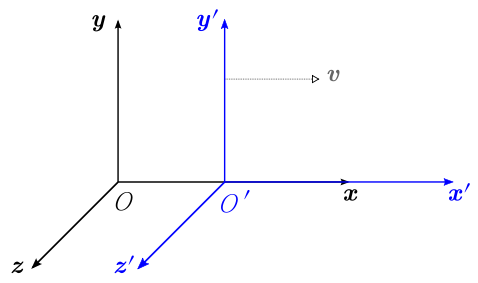
\includegraphics[width=0.5\textwidth]{physics/images/relativity}}

With relativity, we always talk about "frames" which are just places that you, as an observer would see things from. Galilean relativity (or "common sense" relativity) says that if you have light of speed $c$ in one frame $F$, which is moving at speed $v$ towards an observer in frame $F'$, the speed of light should be 
\begin{align}
    c' = v+ c
\end{align}
If for instance the like was going towards the origin $O$ in frame $F$. This would be \emph{faster} than what Maxwell's equation's say, so something has to give. Einstein fixed this by positing that both \emph{space and time themselves} are changed between frames with different velocities. When you look at something that is moving, it is shrunken in the direction of travel compared to how it sees itself. Additionally the amount of time it takes for an event to take place (ball thrown, clock tick, etc) takes \emph{longer} in the frame that sees the event as moving, than it would in a frame at which the the event takes place at rest. 


To illuminate, lets pretend we have a person on earth (frame $F$) and a person on a spaceship (frame $F'$) moving away from the earth in the positive $x$ direction with speed $v$. The earth measures everything with coordinates $(t,x,y,z)$ and the person on the ship measures everything with coordinates $(t',x',y',z')$. Both of these coordinate systems are \emph{completely normal} in their own frames. If they had a ball on earth and measured it's radius as $r$, the ruler with which they measure it on the ship would say it is the same $r$ when the entire ship, ball, ruler system is moving together. 

Lets pretend that right when the spaceship passes the earth, they are able to align their coordinate system somehow so everything is zero. The usefulness of special relativity is know how everyone on the ship (in $F'$) sees things after doing some mathematics with all of the things you are capable of measuring in $F$. It turns out that the transformation is given by \footnote{do someday, classical HW 3}
\begin{align}\label{lorentzcontract}
    t' &= \gamma\Big(t -\frac{vx}{c^2} \Big)\\
    x' &= \gamma(x - vt)\\
    y' &= y\\
    z' &= z
\end{align}
Where 
\begin{align}
\gamma =\frac{1}{ \sqrt{1-\frac{v^2}{c^2}}  }
\end{align}
% TODO We can remember these equations as follows. In Galilean relativity, after drawing out the frames, we would have
%\begin{align}
%   x' = x - vt
%\end{align}
%Both are modulated by $\gamma$, to keep the expression finite when $v$ gets larger and larger. The sign on the time matches $x$, and must match units and $t$. ...  TODO

We can do something interesting from here, lets look at the following quantity
\begin{align}
    s^2 &= -c^2t'^2 +x'^2 + y'^2 + z'^2\\
    &= \frac{c^2(t^2 - \frac{vx}{c^2})^2}{1-\frac{v^2}{c^2}}  + \frac{(x - vt)^2}{1-\frac{v^2}{c^2}} + y^2 + z^2\\
    &= -c^2t^2 + x^2 + y^2 + z^2
\end{align}
It turns out this quantity is \emph{invariant} when we change between frames. These type of things are incredibly important when dealing with topics in special relativity

\subsection{Four Vectors}
A nice way to write things that give us invariants easily is in four vector notation. We can define the position \emph{contravariant} vector with
$$ x^\mu \equiv (x^0, x^1,x^2,x^3) = (ct,x,y,z) $$
Remember the signs by knowing all the vectors with \textit{upper} indices have all \textit{positive} quantities. We can then define a \emph{covariant} with
\begin{align}
     x_\mu \equiv (-x^0, x^1,x^2,x^3) = (-ct,x,y,z) 
\end{align}
We see that if we dot these two vectors we get 
\begin{align}
    s^2 = x_\mu x^\mu = -c^2t^2 + x^2 + y^2 + z^2
    \end{align}
This one tells us things about how events are causally connected to one another, since

$$s^2 = - c^2(t_2-t_1)^2 + (\textbf{x}_2-\textbf{x}_1)^2$$

\begin{itemize}
\item $s^2 = 0$ Lightlike, only massless particles moving at $c$ will have this 0 
\item $s^2 > 0$ Spacelike, in every frame, there will always be some separation of space between the events. Causally unrelated
\item $s^2 < 0$ Timelike, time separates these events in all frames.
\end{itemize}

Another useful thing that comes up often is the \textbf{Minkowski Metric} defined as 

\begin{align}
\eta_{\mu\nu} = \left(
{\begin{array}{cccc}
-1&0&0&0\\
0&1&0&0\\
0&0&1&0\\
0&0&0&1
\end{array}}
\right)
\end{align}
This transforms a contravariant into a covariant with
\begin{align}
    x_\mu = \eta_{\mu\nu}x^\nu
\end{align}
Also important is the 4-gradient

\begin{align}
\partial_\mu &\equiv \frac{\partial}{\partial x^\mu} = (\frac{\partial t}{\partial x^0}\frac{\partial}{\partial t}, \frac{\partial x}{\partial x^1}\frac{\partial}{\partial x}, \frac{\partial y}{\partial x^2} \frac{\partial}{\partial y},\frac{\partial z}{\partial x^3}\frac{\partial}{\partial z} ) = (\frac{1}{c} \partial_t, \partial_x,\partial_y,\partial_z)
\end{align}

Be aware that the lower index partial is with respect to the upper index $x$. Similarly this gives
$$\partial^\mu = (-\frac{1}{c}\partial_t,\partial_x,\partial_y, \partial_z)$$

\subsection{Relativistic Kinematics}
The key equation to remember is 
\begin{align}\label{relenergy}
    E^2 = p^2c^2 +m^2c^4
\end{align}
We can define the \emph{four momentum} as
\begin{align}
    p^\mu = (E/c,p_x,p_y,p_z)
\end{align}
Notations can sometimes swap the minus signs, but it seems easier to remember that all raised index vectors are entirely positive. The covariant is the same with the front sign swapped. We see that if we rearrange equation \ref{relenergy} we can find
\begin{align}
- m^2c^2 = -\frac{E^2}{c^2} + p^2 = p_\mu p^\mu
\end{align}
Usually in the problems here you are given two objects with momentum $p_1^\mu$ and $p_2^\mu$ respectively, that turn into a new particle with four-vector $p_3^\mu$. We know that in general
\begin{align}
    p_3^\mu = p_1^\mu + p_2^\mu
\end{align}
Which means we just add each of the components of the vector like normal, which gives us the new 4 momentum. From here, we can find the invariant mass of the system just doing
\begin{align}
    -m_3^2c^2 = (p_{1\mu} + p_{2\mu})(p_1^\mu + p_2^\mu)
\end{align}
Proper time is Lorentz invariant and defined as

\begin{equation}\label{propertime}
c^2d\tau^2 = -\eta_{\mu\nu}dx^{\mu}dx^{\nu}
\end{equation}
The 4-velocity is then defined as

$$u^\mu \equiv \frac{d x^\mu}{d\tau}$$
Plugging in our definition back into equation \ref{propertime} we get that 
\begin{align}
-c^2 &= u_\mu u^\nu\\
 &= -c^2\frac{d t}{d \tau}^2 + \frac{d x}{d \tau}^2 + \frac{d y}{d \tau}^2 + \frac{d z}{d \tau}^2\\
 &= -c^2\frac{d t}{d \tau}^2(1- \frac{v^2}{c^2}) 
\end{align}
This gives us time dilation with $\gamma d\tau = dt$. Replugging this into the definition of the 4-velocity, we get

$$u^\mu = (\gamma c, \gamma v_x, \gamma v_y,\gamma v_z)$$
This allows us to then define the 4-momentum of a massive particle as 
$$p^\mu \equiv mu^\mu = (\gamma mc, \gamma mv_x, \gamma mv_y,\gamma mv_z)$$
The Lorentz force equation is given by

$$\frac{dp^\mu}{d\tau} = eF^{\mu\nu}\frac{dx^\nu}{d\tau}$$


There is a similar way to write the boost in momentum and energy as we did for space and time
\begin{align}
    E' &= \gamma(E - vp_x)\\
    p_x' &= \gamma(p_x - vE/c^2)\\
    p_y' &= p_y\\
    p_z' &= p_z
\end{align}
If the other frame $F'$ is moving with velocity $v$ in the $x$ direction relative to frame $F$.


\section{Rotation}\label{classicalrot}



\begin{figure}\label{rotation}
\centerline{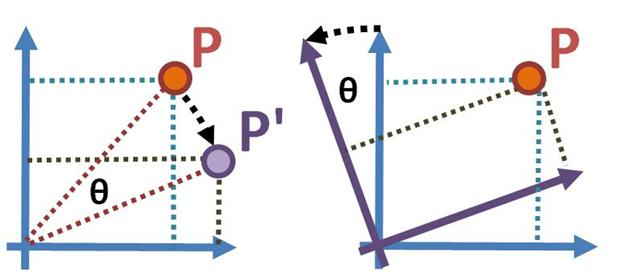
\includegraphics[width=0.7\textwidth]{physics/images/rotation}}
\caption{The left is an \emph{active} rotation, which involves physical rotation of an object. The right is a \emph{passive} rotation which involves instead the rotation of the coordinate system.}
\end{figure}

$$R(\hat{n},\theta)$$

$R$ is a rotation matrix, $\hat{n}$ is what axis you are choosing to rotate around, points along that axis. $\theta$ determines how far around that axis you are going to rotate. Directions are chosen from the cross product, for instance if it is $\hat{z}$, we know $x\times y=z$, so that requires use to have it such that it looks like $x$ chases $y$, or $x$ will move towards $y$ in the direction it is closest to it from. This turns out to happen for all of the pairs, when said in order, i.e.

\begin{align}
x\times y &= z\\
y\times z &= x\\
z\times x &= y\\
\end{align}

If you ever find them in the opposite order, it is equivalent to going the opposite direction. There are two typical conventions for rotations outline in Figure \ref{rotation}. In most cases, we only care about the active rotation, given around the $\hat{z}$ axis below with

\begin{align}
R(\hat{z},\theta) =  \left(
{\begin{array}{ccc}
\cos\theta&-\sin\theta&0\\
\sin\theta&\cos\theta&0\\
0&0&1\\
\end{array}}
\right)
\end{align}

Similar rotations around $\hat{x},\hat{y}$ can be found easily by cyclically permutating the vectors and realigning, with

\begin{align}\left(
{\begin{array}{c}
x_1\\
y_1\\
z_1\\
\end{array}}\right) &\rightarrow
\left(
{\begin{array}{c}
z_1\\
x_1\\
y_1\\
\end{array}}\right) \\
\left(
{\begin{array}{c}
z_1'\\
x_1'\\
y_1'\\
\end{array}}\right) &= 
\left(
{\begin{array}{ccc}
\cos\theta&-\sin\theta&0\\
\sin\theta&\cos\theta&0\\
0&0&1\\
\end{array}}
\right)\left(
{\begin{array}{c}
z_1\\
x_1\\
y_1\\
\end{array}}\right)\\
\rm{Reorder}\implies  
\left(
{\begin{array}{c}
x_1'\\
y_1'\\
z_1'\\
\end{array}}\right)
&= \left(
{\begin{array}{ccc}
\cos\theta&0 &\sin\theta\\
0&1&0\\
-\sin\theta&0&\cos\theta\\
\end{array}}
\right)\left(
{\begin{array}{c}
x_1\\
y_1\\
z_1\\
\end{array}}\right)
\end{align}
This is a rotation around the $\hat{y}$ axis, as that direction is unaffected. 




\subsection{Rotating Frames}
Given a rotating frame $r$ which is rotating with constant angular velocity $\omega$ and we want to find a non-rotating frame $s$ where Newton's laws apply, we have that
\begin{align}
\textbf{v}_s = \textbf{v}_r + \boldsymbol{\omega}\times\textbf{r}
\end{align}
Where $r$ is the distance from the center of rotation. To find the acceleration, we must also consider the unit vectors as a function of time, with %\todo{Fix this, do in index notation}
\begin{align}
\textbf{a}_s = \frac{d\textbf{v}_s}{dt} &= \frac{d}{dt}\Big[|v_x|\hat{x} + |v_y|\hat{y} + |v_z|\hat{z} + \boldsymbol{\omega}\times(|r_x|\hat{x} + |r_y|\hat{y} + |r_z|\hat{z})\Big]\\
&= \Big[|\dot{v}_x|\hat{x} + |\dot{v}_y|\hat{y} + |\dot{v}_z|\hat{z} + \boldsymbol{\omega}\times(|\dot{r}_x|\hat{x} + |\dot{r}_y|\hat{y} + |\dot{r}_z|\hat{z})\Big] \\
&+ \Big[|v_x|\dot{\hat{x}} + |v_y|\dot{\hat{y}} + |v_z|\dot{\hat{z}}  +\boldsymbol{\omega}\times(|r_x|\dot{\hat{x}} + |r_y|\dot{\hat{y}} + |r_z|\dot{\hat{z}})\Big]\\
\end{align}
In general the time derivative of any unit vector in a rotating frame is given by
\begin{align}
\dot{\hat{u}} = \boldsymbol{\omega}\times\hat{u}
\end{align}
We also know that $\dot{r}_i = v_i$ and $\dot{v}_i = a_i$ since they are simply the rate of change of the objects position and velocity. Thus we have
\begin{align}
\textbf{a}_s &= \textbf{a}_r + \boldsymbol{\omega}\times\textbf{v}_r + \boldsymbol{\omega}\times\textbf{v}_r + \boldsymbol{\omega}\times(\boldsymbol{\omega}\times\textbf{r})\\
&= \textbf{a}_r + 2\boldsymbol{\omega}\times\textbf{v}_r + \boldsymbol{\omega}\times(\boldsymbol{\omega}\times\textbf{r})
\end{align}
Now we care about how Newton's laws look in the rotating frame, and rearranging tells us that
\begin{align}
\textbf{a}_r = \textbf{a}_s - 2\boldsymbol{\omega}\times\textbf{v}_r - \boldsymbol{\omega}\times(\boldsymbol{\omega}\times\textbf{r})
\end{align}
So we have the normal acceleration that would be created from Newton's second law in a non-rotating frame, then two extra terms which are caused by the rotation of the frame itself. The first term is the Coriolis acceleration, and the second is centrifugal acceleration.


\subsection{Moment of Inertia}
To find the moment of inertia of a simple object positioned in a difficult way, first find the moment of inertia of the body in it's center of mass frame such that the tensor is diagonal such that 

$$ I_{CM} = 
\left(
{\begin{array}{ccc}
I_{xx}&0&0\\
0&I_{yy}&0\\
0&0&I_{zz}\\
\end{array}}
\right)$$

With this you can then rotate the tensor to find what it would be if the object is spun on a more difficult axis. with 

$$I_{Rot} = R(\theta_x)R(\theta_y)R(\theta_z)~I_{CM}~R(\theta_z)^{-1}R(\theta_y)^{-1}R(\theta_x)^{-1}$$

If the axis is still not where you want it to be, just apply the parallel axis theorem to again shift it with

$$I_{F} = I_{Rot} + Md^2$$





\section{Fluid Mechanics}
Fluid Mechanics is right on the border of being classical mechanics and statistical mechanics. It has to do with how a large number of particles move together. Looking at the mass density $\rho$, because we cannot create or destroy mass classically, we have
\begin{equation}\label{masscon}
\frac{\partial\rho}{\partial t} = -\nabla\cdot (\rho\textbf{v})
\end{equation}
Which is just the continuity equation, and says that the rate at which the mass density is shrinking is equal to how much mass is leaving each surface at a given time. We also define the momentum of a system by adding up each infinitesimal mass and multiplying it by its respective velocity. This is the same thing as 
\begin{align}
    \textbf{p}(V,t) = \int_V dx^3 \rho(\textbf{x},t)\textbf{v}(\textbf{x},t)
\end{align}
An important thing to note is that the velocity $\textbf{v}$ in the integral is not specifically the velocity of any one particle, but called a \emph{velocity field} since it is defined over the entire volume, and the particles are too small for us to be concerned about any of them individually. Newton's third law tells us that $\textbf{F} = \dot{\textbf{p}}$, so we first define the \emph{force field}
\begin{align}
    \textbf{F}(V,t) = \int_V dx^3 \textbf{f}(\textbf{x},t)
\end{align}
Let's match Newton's third law and find
\begin{align}
    \int_V dx^3 \textbf{f}(\textbf{x},t) &= \frac{d}{dt}\int_V dx^3 \rho(\textbf{x},t)\textbf{v}(\textbf{x},t)
\end{align}
Conservation of momentum (also called Euler's equations) gives us
\begin{equation}\label{momcon}
\rho\left({\frac{\partial\textbf{v}}{\partial t} + (\textbf{v}\cdot\nabla)\textbf{v}}\right) = \textbf{f}
\end{equation}
%TODO Some more trivia
%
%\begin{itemize}
%\item Ideal Fluids
%\begin{itemize}
%\item Force field given by $\textbf{f} = -\nabla p$
%\item Isentropic Flow
%\begin{itemize}
%\item Kelvin's Theorem $\frac{d}{dt}\oint \delta\textbf{x}\cdot\textbf{v} = 0$
%\end{itemize}
%\end{itemize}
%\item Incompressible Fluids -  ($\rho=$ const, $\nabla\cdot \textbf{v} = 0$)
%\item Steady Flow -  $d\textbf{v}/dt = 0$
%\item Potential Flow $\textbf{v} = \nabla\phi$
%\end{itemize}
%If any coordinate goes to infinity ($\textbf{v}\cdot\nabla)\textbf{v} = 0$
%

%\section{TODO}

%\begin{itemize}

%\item Classical HW6 Problem 1, coupled oscillators
%\end{itemize}




\chapter{Statistical Mechanics and Thermodynamics}



\section{Laws of Thermodynamics}
\begin{enumerate}
\item The change in \emph{internal} energy of a system is equal to the heat added minus the work it does
\begin{align}
dE = \delta Q - \delta W
\end{align}
The reason why we write the squiggles is because this is true no matter how you change the system, as we must still have conservation of energy, but if we have cases where we move between equilibriums we can then write that $\delta Q = T dS$ and $\delta W = PdV$. In general $TdS \ge \delta Q$, for instance a freely expanding gas, which does not exchange heat, but since it has more places for each molecule to be, increases in entropy.


\item Entropy of the universe always increases

$$\Delta S \ge 0$$ Is a statement that the equilibrium state is preferred for a system, so if a system is changed, it is at first not in equilibrium, then moves towards equilibrium, where the entropy is maximized, so the change in entropy will be increased. Equilibrium can be thought of as a state where any process and its time reversal have equal probability. \textbf{Detailed Balance} says that if you have two processes (1,2) $\rightarrow$ (3,4) they are just as likely as (3,4) $\rightarrow$ (1,2)


\item Entropy of a perfect crystal (one state) goes to zero as temperature goes to zero
 $$S\rightarrow 0 ~~\rm{as}~~ T\rightarrow 0$$

\end{enumerate}

\section{Thermodynamics}
Thermodynamics has to do with huge numbers of particles that we can't easily keep track of individually. For classical mechanics, our "state variables" were things like positions and momentum in the Hamiltonian formulation. In Thermodynamics,  instead of trying to keep track of $10^{23}$ pairs of position and momenta, we just keep track of a few macroscopic things that can tell us things about the system from a macroscopic point of view. 

Here our "state variables" are $p,T,V,S$ out of which we are able to describe everything. %\footnote{I'm not entirely sure why these were chosen., as entropy itself is non-trivial to measure, maybe its the leftover variable?} 
The issue is that these variables  are all netted together in often mathematically unfriendly ways and in general are \emph{not independent} of one another. We get around this by just taking a bunch of partial derivatives all over the places, holding this or that constant.

We start with the first law of Thermodynamics
\begin{align}
dE = \delta Q - \delta W
\end{align}
So long as each time we infinitesimally change the system, we wait for it to equilibrate before touching it again (a \emph{quasistatic process}),  we can use the equalities
\begin{align}
dE = TdS - p dV
\end{align}
In general
\begin{align}
T\delta S \ge \delta Q
\end{align}
This is because entropy can change without heat being added to the system, for instance a free expansion of a gas. Rearranging the first law to find entropy, we get
\begin{align}
dS &= \frac{1}{T}dE +\frac{p}{T}dV
\end{align}
We are also free to think of the energy as being a function of $T$ and $V$, so
\begin{align}\label{thermenergy}
dE = \Big(\frac{dE}{dT}\Big)_VdT + \Big(\frac{dE}{dV}\Big)_TdV
\end{align}
Which tells us
\begin{align}
dS &= \frac{1}{T}\Big(\frac{dE}{dT}\Big)_VdT + \frac{1}{T}\Big[p + \Big(\frac{dE}{dV}\Big)_T\Big]dV
\end{align}
But also
\begin{align}
dS &= \Big(\frac{dS}{dT}\Big)_V dT + \Big(\frac{dS}{dV}\Big)_T dV
\end{align}
Which shows us one of the many funny relationships we get with the partial derivatives
\begin{align}
 \Big(\frac{dS}{dT}\Big)_V &= \frac{1}{T}\Big(\frac{dE}{dT}\Big)_V\\
\Big(\frac{dS}{dV}\Big)_T &= \frac{1}{T}\Big[p + \Big(\frac{dE}{dV}\Big)_T\Big]\label{partialentropy}
\end{align}
Going back to equation \ref{thermenergy}, by definition, we have the specific heat as
Part of this is easy since by definition
\begin{align}
c_v \equiv \Big(\frac{dQ}{dT}\Big)_V = \Big(\frac{dE}{dT}\Big)_V
\end{align}
For the next one, we can rearrange equation \ref{partialentropy} after using the Maxwell square (Section \ref{square}) to find
\begin{align}
\Big(\frac{\partial S}{\partial V}\Big)_T &= \Big(\frac{\partial p}{\partial T}\Big)_V
\end{align}
Plugging this in we get
\begin{align}
T\Big(\frac{\partial p}{\partial T}\Big)_V - p = \Big(\frac{dE}{dV}\Big)_T
\end{align}
Which is often useful when given an equation of state i.e. function that contains $P$ as a function of the other variables. I still don't have a solid grasp as to the best algorithm for finding these relationships, it seems like trying to get somewhere by random walk.



\subsection{Thermodynamic Potentials}
The idea here is that somehow from the second law, you can write all of these different kinds of potentials which are at a minimum when we 
hold certain things about the system as constant. \\

\begin{center}
\begin{tabular}{ c c }
Constant & Potential Minimized \\ \hline
$S,V$ & $U$ - Internal Energy\\
$T,V$ & $F$ - Helmholtz Free Energy\\  
$T,P$ & $G$ - Gibbs Free Energy \\
$S,P$ & $H$ - Enthalpy\\
$T,V,\mu$ & $\Phi$ - Grand Potential  
\end{tabular}
\end{center}
So what we do with each of these guys is, since we know two of the things are constant, we take the derivative of the potential with respect to either of the other two state variables and set it to zero. We can then solve that equation for whatever we are looking for. The Helmholtz free energy can be written as

\begin{align}
F = U - TS = -kT\ln Z
\end{align}



\subsection{Thermodynamic Square}\label{square}

As a reminder
\begin{align}
U=&~\textrm{Internal Energy}\\
H =&~\textrm{Ent\textbf{h}alpy}\\
G =&~\textrm{\textbf{G}ibbs Free Energy}\\
F =&~\textrm{Helmholtz \textbf{F}ree Energy}
\end{align}
A nice mnemonic for remembering:\\ \\
\centerline{Good Physicists Have Studied Under Very Fine Teachers.}
\\
\\
\centerline{\includegraphics[width=0.3\textwidth]{physics/images/Thermodynamic_square}}
\begin{enumerate}
\item Start with a potential (e.g. $F$)
\item Pick the two variables at the opposite corners, noting their signs (e.g. $-P$, $-S$)
\item Now multiply those terms by their term furthest from them, forgetting about the sign. This gives us $$dF = -S dT -pdV$$
\item If you have non-fixed number of particles, just add $+\mu dN$ to whichever potential you are looking at
\end{enumerate}

This gives us the natural way to express whatever potential we obtained, in terms of the differentials, so
\begin{align}
F = F(T,V)
\end{align}

We can also obtain the maxwell relations with the square once we find the definition of the potential we chose, we can say
\begin{align}
dF = \Big(\frac{\partial F}{\partial T}\Big)_V dT + \Big(\frac{\partial F}{\partial V}\Big)_T dV
\end{align}
We know by definition that
\begin{align}
\frac{\partial^2 F}{\partial T\partial V} = \frac{\partial}{\partial V}\Big(\frac{\partial F}{\partial T}\Big)_V &= \frac{\partial}{\partial T}\Big(\frac{\partial F}{\partial V}\Big)_T 
\end{align}
So looking at the prefactors on our initial expression for the potential, we can find that
\begin{align}
-\Big(\frac{\partial S}{\partial V}\Big)_T &= -\Big(\frac{\partial p}{\partial T}\Big)_V
\end{align}
We can do the same trick to find the rest, there is one for each potential. You can also look and see you can obtain these factors by taking a ''U" shape in the box. In the above case we take the top row, then the bottom right corner, is equal to the bottom row, then the top right corner.


\section{Quasi-Static (Reversible) Process}

$$\Delta S = 0$$
As the system changes, it does so by changing between equilibrium states the entire time. Because it is in equilibrium the entire time, we don't change entropy. 


\section{Ideal Gas}
An ideal gas is just a gas that doesn't interact with the other molecules in the gas, and behaves as if each of the molecules were just alone. We calculate the partition function for just one of the particles with
\begin{align}
    Z_1 = \frac{1}{h^3}\int dx^3 \int dp^3 e^{-\beta p^2/2m}
\end{align}
Which is just adding up all the possible states it could be in. It's energy is just kinetic. We can actually evaluate this integral explicitly using a Gaussian integral trick giving us
\begin{align}
    Z_1 = \frac{V}{h^3}\Big(2\pi m kT\Big)^{3/2}
\end{align}
Since the particles don't interact, the total partition function, which is the normalizing factor considering \emph{all} states, is just all of the individual ones multiplied together, normalized by $1/N!$ due to a strange paradox called the Gibb's paradox.
\begin{align}
    Z = \frac{1}{N!} Z_1^N = \frac{V^N}{h^3N!}\Big(2\pi m kT\Big)^{3N/2}
\end{align}
The free energy of a system is defined as 
\begin{align}
    F = -kT\ln Z
\end{align}
And we know that one of Maxwell's relations tells us 
\begin{align}
    P = -\Big(\frac{dF}{dV}\Big)_{T,N}
\end{align}
This formula in general tells us the \emph{equation of state} and is true for any type of system. Using our expression for the partition function and plugging into this, we can find the equation of state for an ideal gas, which we all know and love
\begin{align}
    PV = NkT
\end{align}
\subsection{Isotherms}
From the equation of state, we see that if temperature is constant for a process, we must have that the product of pressure and volume is also constant
\begin{align}
    PV = \textrm{const}
\end{align}

\subsection{Adiabats}
Adiabatic expansion happens when there is no heat transferred to or from the system, so
\begin{align}
    \delta Q = 0
\end{align}
So looking at the first law, we see
\begin{align}
    dU = -PdV
\end{align}
We know for an ideal gas, the internal energy $U$ is only dependent on temperature, and after also plugging in for the ideal gas law
\begin{align}
    \frac{3}{2}Nk dT = -\frac{NkT}{V}dV
\end{align}
Rearranging and integrating we see that
\begin{align}
    \int \frac{dT}{T} &= -\frac{2}{3} \int \frac{dV}{V}\\
    \ln T &= -\frac{2}{3}\ln V + C
\end{align}
Exponentiating, we have
\begin{align}
    TV^{2/3} = e^C
\end{align}
Now plugging in the equation of state once more, we arrive at
\begin{align}
    PV^{5/3} = Nke^C
\end{align}
Or, since the number of particles is held fixed, we have that 
\begin{align}
    PV^{5/3} = \textrm{const}
\end{align}

\subsection{Free Expansion}
In a free expansion, the gas does no work, so
\begin{align}
    dW = 0
\end{align}
and if the process is adiabatic
\begin{align}
    dQ = 0
\end{align}
Which tells us the change in internal energy is zero
\begin{align}
    dU = dQ - dW
\end{align}
So with the ideal gas law, we get
\begin{align}
    P_iV_i = P_fV_f
\end{align}

\section{Entropy}

Entropy can be thought of as a unit of information. The mathematical definition of entropy is given by

\begin{align}\label{entropy}
S = k_B\ln\Omega
\end{align}
Where $\Omega$ is the number of possible ways a given system could be arranged, each with equal probabilities. The entropy is a state variable, and can be evaluated explicitly for a given system, i.e. a system will have a definite entropy. What we mean by "number of ways the system could be arranged" is the amount of configurations we could put all of the small pieces together that make up the system (typically all the molecules) that give us the exact same macroscopic quantities. %\todo{elaborate}



 The second law tells us that number of ways that the universe could be organized is \emph{always} increasing in time until it reaches equilibrium. There is speculation that this should in some way tell us more about time itself, as the two are entwined together in way a which is still one of Physics great mysteries\cite{weinert}. Another more general definition is given by

\begin{align}\label{gen-entropy}
S = -\sum_{i=1}^N P_i\ln P_i
\end{align}

Where we sum over the probabilities that the system is in the state $1,2,... N$. For instance if there are two energies ($0,\epsilon$) possible, you will sum over those states for the entropy. This definition must also include states which are degenerate in energy. The reason for the minus sign is that the logarithm of a fraction is negative, so to get entropy positive, we swap signs. This expression reduces to equation \ref{entropy} in the case where all the probabilities are equal. 

The entire game of statistical mechanics boils down to try to maximize this quantity (equation \ref{gen-entropy}) under constraints using Lagrange multipliers. Two simple constraints are

\begin{align}\label{sumprob}
\sum_{i=1}^N P_i -1 &= 0\\ \label{sumenergy}
\sum_{i=1}^N E_iP_i - E &= 0\\
\end{align}
These are the constraints for the canonical ensemble. So using the multipliers
\begin{align}
S' = -\sum_{i=1}^N P_i\ln P_i - \alpha\Big[\sum_{i=1}^N P_i -1\Big] - \beta\Big[\sum_{i=1}^N E_iP_i - E\Big]
\end{align}
We now look for the extremum of the entropy, which will be positive since $P_i$ is always positive, and $-\ln P_i$ is also always positive. 
\begin{align}
\frac{\partial S'}{\partial P_i} &= -\ln P_i  + 1 -\alpha - \beta E_i\\
 &= 0 
\end{align}
We see we have now almost accidentally obtained an expression for each $P_i$, which we can get by shifting variables and exponentiating. We first define $1-\alpha = \ln Z$

\begin{align}\label{stat-probability}
P_i = \frac{1}{Z}e^{-\beta E_i}
\end{align}
This is the \textbf{Boltzmann distribution}, found only using the constraint of maximum entropy, total energy, and probability conservation. This allows us to define the \textbf{partition function} $Z$ plugging into equation \ref{sumprob} with
\begin{align}
\sum_{i=1}^N e^{-\beta E_i} = Z
\end{align}
Which acts like a normalization factor for the probabilities. Now plugging into equation \ref{sumenergy}, we get

\begin{align}
\sum_{i=1}^N \frac{1}{Z}e^{-\beta E_i}E_i = E
\end{align}
We now see that the following identity holds, which lets us express the average energy as a function of \emph{only} the partition function
\begin{align}\label{partenergy}
E = -\frac{1}{Z}\frac{\partial Z}{\partial \beta} = -\frac{\partial \ln Z}{\partial \beta}
\end{align}
In the continuum limit, we get 

\begin{align}
S = -\int dV \rho \ln\rho
\end{align}

Where $\rho$ is the \emph{probability density} and we integrate over the volume in phase space $p,q$ as we define the states as when an atom has some fixed $p, q$. This has an identical form to the density matrices  used in Quantum Mechanics (Equation \ref{density}), which is pretty weird.




\section{Temperature}
Temperature is the measure of the average kinetic energy of a system. It is defined as 

\begin{align}
\frac{1}{T}= \frac{\partial S}{\partial E}
\end{align}

It tells you how much the entropy changes by when you change the average energy of the system. It can be shown using equation \ref{stat-probability} that the entropy looks like
\begin{align}
S = k(\beta E + \ln Z)
\end{align}
Thus
\begin{align}
dS &= Ed\beta + \beta dE +\frac{\partial \ln Z}{\partial \beta}d\beta\\
&= Ed\beta + \beta dE -Ed\beta\\
&= \beta dE
\end{align}
Which tells us that
\begin{align}
\frac{1}{T} = \beta
\end{align}
So temperature is in fact just a Lagrange Multiplier.


\section{Partition Function}
The real secret behind getting good at statistical mechanics is just getting fancy with how you take derivative of the partition function. For instances let's look at the specific heat capacity
\begin{align}
    C_v = \frac{\partial \langle E\rangle}{\partial T} &= \frac{\partial}{\partial T}\Big[\frac{1}{Z}\sum_{i=1}^N E_i e^{-E_i/kT}\Big]\\
    &= -\frac{1}{Z^2}\sum_{i=1}^N E_i e^{-E_i/kT}\frac{\partial Z}{\partial T} + \frac{1}{kT^2Z}\sum_{i=1}^N E_i^2 e^{-E_i/kT}
\end{align}
It can be shown that eventually we get an expression that relates the specific heat capacity to the \emph{average fluctuations in energy} which is super weird.
\begin{align}
    \langle \Delta E^2\rangle= C_vkT^2 
\end{align}

\section{Ensembles}
Usually when we need statistical mechanics, it is because we care about how fast a block of ice melts or the spreading out of a gas. These objects of interest are called \emph{systems}. %TODO Because statistical mechanics is all about averages, \footnote{Kittel pg. 9}

\subsection{Microcanonical Ensemble}
Here, because the system can have only one energy level, we look for states within that energy $E$, again using Lagrange multipliers with
\begin{align}
    S' = -\sum_{i=1}^N P_i\ln P_i - \alpha\Big[\sum_{i=1}^N P_i -1\Big]
\end{align}
Taking the derivative, we see that
\begin{align}
    \frac{\partial S'}{\partial P_i} &= -\ln P_i  + 1 -\alpha\\
 &= 0 
\end{align}
So the probability that the system is in any of it's states with total energy $E$ is given by a constant, with
\begin{align}
    P_i = e^{1-\alpha} = \frac{1}{Z}
\end{align}

%\subsection{Canonical Ensemble}

\subsection{Grand Canonical Ensemble}% \todo{this is garbage}
We now pretend we have a system $A$ with $N_r$ at energy $E_s$ which is free to exchange particles and everything with another system $A'$ at $E_s'$. Under the constraints that
\begin{align}
E_i + E_i' = E^{(0)}\\
N_r + N_r' = N^{(0)}
\end{align}
We have different indices for the energy and particle number because there can be states with differing number of particles $N_r$ which all have the same energy $E_i$. Our task is to find the probability $P_{i,r}$ that the system $A$ is in some given state $E_i$ with number of particles in it $N_r$. It is legitimate to think that this probability should be proportional to the amount of ways you can organizes all the molecules and their energy to get exactly the energy in the \emph{other} system $A'$ to be $E^{(0)} - E_i$
\begin{align}
P_{i,r}(E_i,N_r) \propto \Omega'(E^{(0)} - E_i , N^{(0)}- N_r)
\end{align}
We are also going to pretend the system $A$ is much smaller than the other, so $E_i\ll E^{(0)}$ and $N_r \ll N^{(0)}$, which lets us Taylor expand the number of ways we can arrange the system, after taking the natural log to keep it's extensive nature.
\begin{align}
\ln\Omega'(E^{(0)} - E_i , N^{(0)}- N_r) = \ln\Omega'(E^{(0)},N^{(0)}) - \Big[\frac{\partial\ln\Omega'}{\partial E'}\Big] E_i - \Big[\frac{\partial\ln\Omega'}{\partial N'}\Big]N_r
\end{align}
From here, we identify constants as 
%\footnote{There is likely a better way to do all of this, but I haven't found it}
\begin{align}
\Big[\frac{\partial\ln\Omega'}{\partial E'}\Big] = \frac{1}{kT}&&\Big[\frac{\partial\ln\Omega'}{\partial N'}\Big] = -\frac{\mu}{kT}
\end{align}
Exponentiating the expression, we see that 
\begin{align}
P_{i,r}\propto\exp\Big[-\beta(E_i-\mu N_r)\Big]
\end{align}
We can then normalize everything to find that
\begin{align}
P_{i,r} = \frac{e^{-\beta(E_i-\mu N_r)}}{\sum_{i,r}e^{-\beta(E_i-\mu N_r)}}
\end{align}




\section{Distributions}
To obtain the distributions, we discretize each of the energies, which is what happens from Quantum Mechanics. For a given energy level of the entire system $E_i$, it should be the sum of the number of particles in each discretize energy level $\epsilon$ multiplied by $\epsilon$ itself.

\begin{align}
    E_i = n_1\epsilon_1 + n_2\epsilon_2 + n_3\epsilon_3 + ...
\end{align}


We also assume that there is some function $\mu$ called the \emph{chemical potential} which tells us how much energy it takes to add another particle to the system. The total energy from the chemical potential $\mu$ is given by
\begin{align}
    \mu N = \mu(n_1 + n_2 + n_3 + ... ) 
\end{align}
This gives us our full partition function as 
\begin{align}
Q= \sum e^{-\beta(n_1\epsilon_1  +  n_2\epsilon_2 +  n_3\epsilon_3 + ...) + \beta\mu(n_1 + n_2 + n_3 + ...)}
\end{align}
Where the different $n$'s are how many particles are in each of the discretized energy levels. We of course also have the constraint that
\begin{align}
n_1 + n_2 + n_3 + ... = N
\end{align}
This partition function is actually huge in general, because each of the $n_1, n_2,$ etc are currently \emph{unbounded} and could be any number. So the sum has to be over all possible combinations of them.
Thankfully however, we are free to break up the partition function however we like as long as we eventually enumerate over all the possible states. To show this, let's pretend that we have only two energy levels $\epsilon_1, \epsilon_2$ making the full partition function
\begin{align}
    Q_T = \sum_{n_1}\sum_{n_2}e^{-\beta[n_1\epsilon_1 + n_2\epsilon_2 - \mu(n_1 + n_2)]} = \sum_{n_1} e^{-\beta(\epsilon_1-\mu)n_1} \sum_{n_2} e^{-\beta(\epsilon_2 - \mu)n_2} = Q_1Q_2
\end{align}
So in fact the total partition function is just the \emph{product} of each of the individual ones. Lets break up the partition function for how many particles $n_k$ are in the $k$th energy level $\epsilon_k$, so
\begin{align}
Q = \prod_k Q_k
\end{align}
This gives us the partition function for the number of particles in each discrete energy level $\epsilon_k$ as 
\begin{align}
Q_k = \sum_{n} e^{-\beta(\epsilon_k - \mu)n}
\end{align}
Where we sum over $n$, which can take on as many values as are allowed for that discrete level. From here, we can do some playing around with the mini partition function $Q_k$ to find the average amount of particles in the discretized state $\epsilon_k$ is
\begin{align}
    \langle n_k \rangle = \sum_n nP_n = \frac{1}{Q_k} \sum_n n e^{-\beta(\epsilon_k-\mu)n}
\end{align}
We see that this is basically the same thing as taking the derivative of the partition function $Q_k$. Working everything out, we find

\begin{align}\label{occupation}
\langle n_k \rangle  =\frac{1}{\beta Q_k}\frac{\partial Q_k}{\partial \mu} = \frac{1}{\beta}\frac{\partial \ln Q_k}{\partial \mu}
\end{align}

\subsection{Fermi-Dirac}
In Fermi Dirac statistics, because of the Pauli Exclusion principle, we have to have that
\begin{align}
n_k = 0~\rm{or}~1
\end{align}
I.e. there can only be a maximum of one particle in each of the given energy levels.
The partition function $Q_k$ is calculated looking at all possible permutations of states and values of $n_k$, but there are only two possibilities, giving us
\begin{align}
Q_k= 1 + e^{-\beta(\epsilon_k-\mu)}
\end{align}
To calculate the average number of particles at the given energy level, we can just plug this into equation \ref{occupation} to find the average number of particles at a given energy to be

\begin{align}
\langle n_k \rangle =\frac{1}{e^{\beta(\epsilon_k - \mu)} + 1}
\end{align}
 This makes sense as it will never be less than 1 in most standard cases.

\subsection{Boltzmann}
This is the classical distribution expressed as
\begin{align}
    p_i\propto e^{-\epsilon_i/kT}
\end{align}
\subsection{Bose-Einstein}
Here there can be \emph{any} number of particles in the same state, so the sum goes to infinity. Making the partition function look like
\begin{align}
    Q_k = \sum_{n=0}^\infty e^{-\beta(\epsilon_k - \mu)n} = \sum_{n=0}^\infty \Big(e^{-\beta(\epsilon_k - \mu)}\Big)^n
\end{align}
We recognize that the number inside the exponent $n$ will always be less than $1$, so this is in fact a Geometric series, giving us
\begin{align}
    Q_k = \frac{1}{1 - e^{-\beta(\epsilon_k - \mu)}}
\end{align}
Taking the same derivative with equation \ref{occupation}, we get
\begin{align}
\langle n_k\rangle = \frac{1}{e^{\beta(\epsilon_k-\mu)}-1}
\end{align}
We see that as $\beta = 1/T \rightarrow \infty$ the occupation number will explode and there will be tons of particles in the state $n_k$. Another important fact is that for photons, chemical potential $\mu = 0$. 


\subsection{Bose-Einstein Condensate} %\todo{might have some errors here}
Since there is not limit to how many bosons can occupy the same state, there is a certain temperature at which nearly all the particles are "condensed" to the lowest possible state. This is the Bose- Einstein Condensate. The math to figure this out is very tricky. How we will find this temperature is first looking at the average number of molecules in all the excited states. We do this by simply adding up the average number of particles in each energy level. In integral form
\begin{align}
    N_e = \int d\epsilon_i \frac{g_i}{e^{\beta(\epsilon_i - \mu)} -1}
\end{align}
Where we have already used the average number of particles in each energy level as
\begin{align}
    \langle n_i\rangle = \frac{1}{e^{\beta(\epsilon_k-\mu)}-1}
\end{align}
The real interesting thing about the Bose Einstein condensate come from the \emph{dimensionality of the phase space}. We will get different results for the critical temperature depending on the phase space allocated to the particles themselves. Let's calculate the the number of particles in the excited state in three dimensions, and just normal kinetic energy
\begin{align}
    N_e &= \frac{1}{h^3}\int dp^3\int dx^3 \frac{1}{e^{\beta(p^2/2m - \mu)} -1}\\
    &=\frac{4\pi V}{h^3} \int_0^\infty  dp \frac{p^2}{e^{\beta(p^2/2m - \mu)} -1}
\end{align}
Remember, the ground state does \emph{not} contribute to this sum since the energy is zero. The integral looks quite intimidating, so we have to use some tricks to evaluate it. Let's start by factoring out the denominator
\begin{align}
    N_e &= \frac{4\pi V}{h^3} \int dp \frac{p^2}{e^{\beta(p^2/2m - \mu)}}\frac{1}{1-e^{-\beta(p^2/2m - \mu)}}
\end{align}
Now the energy is always going to be greater than the chemical potential $\mu$, so the right term is in fact a Geometric series, in the same way we first wrote the Bose - Einstein distribution
\begin{align}
    N_e &= \frac{4\pi V}{h^3} \int dp \frac{p^2}{e^{\beta(p^2/2m - \mu)}}\sum_{n=0}^\infty e^{-\beta n(p^2/2m - \mu)}\\
    &=\frac{4\pi V}{h^3} \int dp ~p^2 \sum_{n=0}^\infty e^{-\beta (n+1)(p^2/2m - \mu)}
\end{align}
Now we shift the order of the sum and the integral, and shift the start of the sum, so we get
\begin{align}
    N_e &= \frac{4\pi V}{h^3}\sum_{n=1}^\infty e^{\beta n\mu}\int_0^\infty dp~p^2  e^{-\beta n p^2/2m}
\end{align}
We can evaluate this integral just doing our normal Gaussian integration after taking the derivative (see the math section) to find
\begin{align}
    N_e &= \frac{4\pi V}{h^3}\sum_{n=1}^\infty e^{\beta n\mu} \frac{\sqrt{\pi}}{4}\Big(\frac{2m}{\beta n}\Big)^{3/2}\\
    &= V\Big(\frac{2\pi m}{h^2\beta}\Big)^{3/2}\sum_{n=1}^\infty \frac{e^{\beta n\mu}}{n^{3/2}}
\end{align}
Since the ground state energy is zero, and it is necessary that $\epsilon - \mu > 0$ for all energies, we need that
\begin{align}
    \mu < 0
\end{align}
Looking the largest possible value this sum could be (where $\mu = 0$), we get the definition of the Riemann Zeta function (See ...)
\begin{align}
    N_e = V\Big(\frac{2\pi m}{h^2\beta}\Big)^{3/2}\sum_{n=1}^\infty \frac{1}{n^{3/2}} &= \Big(\frac{2\pi m kT}{h^2}\Big)^{3/2} \zeta(3/2)
\end{align}
So this is the \emph{maximum} number of particles that we can fit into a volume $V$ at temperature $T$ in the excited states when there is no chemical potential between the molecules, meaning we are free to add or subtract as many as we want. The question becomes, where do they go? Into the ground state. We must have that 
\begin{align}
    N = N_0 + N_e
\end{align}
The first fill up the excited states before condensing to the ground state. We defined a critical temperature at which all the particles go into the excited states before the condensate starts to form with %\todo{fix}
\begin{align}
    N &= \Big(\frac{2\pi m kT_c}{h^2}\Big)^{3/2} \zeta(3/2)
\end{align}
Which let's us find the critical temperature with
\begin{align}
    T_c = \Big(\frac{N}{V\zeta(3/2)}\Big)^{2/3} \frac{2\pi\hbar^2}{mk}
\end{align}
Thus
\begin{align}
    N_0 = N\Big[1-\Big(\frac{T}{T_c}\Big)^{3/2}\Big]&& T < T_c
\end{align}
With these types of integrals we will \emph{always} get something with the Zeta function, the smallest dimensionality that barely won't converge is 
\begin{align}
    \zeta(1) = 1 + \frac{1}{2} + \frac{1}{3} + \frac{1}{4} + ...
\end{align}
Which is the Harmonic series, which does not converge, which tells us that the Bose-Einstein condensate cannot form in one dimension. Apparently the evolution of many complex systems, including the World Wide Web follow Bose statistics and can under go Bose-Einstein condensation \cite{biancoli}.

\subsection{Stefan-Boltzmann Law}
From the partition function for a photon gas, we can get a function for the average energy of a photon gas as usual. Remember that the energy of a photon is $\epsilon = |\textbf{p}|c$, since they don't have mass. Eventually we find that the power, which is energy per unit time goes as 
\begin{align}
    P = A\varepsilon \sigma T^4
\end{align}
This tells us the power radiated from a black-body, (which just means it absorbs everything that hits it) is proportional to the temperature to the fourth power. $A$ is the surface area of the object, $\varepsilon$ is the emissivity, which is 1 if it is a perfect blackbody, and $\sigma$ is a constant from the partition function.

\subsection{Gas - Liquid - Solids}
An Einstein solid assumes all atoms oscillate in all directions with the same frequency $\omega$. We can easily calculate the partition function for one of particles in one of the dimensions, knowing that the energy goes as a harmonic oscillator
\begin{align}
    Z_0 &= \sum_{n=0}^\infty e^{-\beta\hbar\omega(n+1/2)}\\
    &= e^{-\beta\hbar\omega/2} \sum_{n=0}^\infty e^{-\beta\hbar\omega n}\\
    &= \frac{e^{-\beta\hbar\omega/2}}{1-e^{-\beta\hbar\omega}}\\
    &= \frac{1}{2\sinh(\beta\hbar\omega/2)}
\end{align}
We assume all of these oscillators are independent, so to get the full wave function, we just have to exponentiate this 3 times, for each dimension of the single atom, then $N$ to consider all of the atoms in the solid.
\begin{align}
    Z = Z_0^{3N}
\end{align}
Einstein solid particles are said to be distinguishable, so the partition function is not weighted by $1/N!$

\subsection{Chemical Potential}
We know that if we add up the average number of particles in each energy level, we should simply get back the total number of particles, which is a constant if particles are not allowed to leave. For both Fermi and Bose statistics we have
\begin{align}
    N = \sum_{i=0}^\infty \frac{1}{e^{\beta(\epsilon_i - \mu)} \pm 1}
\end{align}
 Let's first consider the Fermi case (with the plus sign). If we look at zero temperature, or $\beta = \infty$, we see that if 
\begin{align}
    \epsilon_i < \mu  && n_i \sim \frac{1}{e^{-\infty} +1} = 1\\
    \epsilon_i > \mu  && n_i \sim \frac{1}{e^{\infty} +1} = 0
\end{align}
Trying the same thing for the Bose case
\begin{align}
    \epsilon_i < \mu  && n_i \sim \frac{1}{e^{-\infty} -1} = -1
\end{align}
We obviously can't have an expectation value of a negative particle
%\footnote{Could this actually account for antiparticles?}
, so the previous expression is wrong, the only valid energies must be
\begin{align}
    \epsilon_i > \mu && n_i\sim \frac{1}{e^{\infty} -1} = 0
\end{align}
But since we need to conserve particle number, we must have that all the particles  have the same energy with
\begin{align}
    \epsilon_i = \mu && n_i = N
\end{align}
This is another way to see Bose-Einstein condensation. %\todo{Verify this last part.}


\subsection{Averages}
For some reason if we want to find the average of a quantity that obeys Fermi or Bose statistics, we can use
\begin{align}
    \langle A \rangle = \frac{1}{(2\pi\hbar)^3}\int d^3p \int d^3r A~\frac{g(E_{pr})}{e^{\beta(E_{pr} - \mu)}\pm 1}
\end{align}

\section{Fermi Energy}
Within a box of length $L = L_x = L_y = L_z$, from quantum mechanics, we know we can expression the energy of any given state as
\begin{align}
E = \frac{\hbar^2\pi^2}{2mL^2}\Big(n_x^2+n_y^2+n_z^2\Big)
\end{align}
We can see these energy levels are degenerate, so it is conventional to imagine something called the "Fermi Sphere" which shifts the $n$'s to spherical geometry, with
\begin{align}
n^2 = n_x^2 + n_y^2+n_z^2
\end{align}
Since the $n$'s must always be positive, we take only the positive quadrant, so $1/8$th of the sphere. Since an electron can be in two spin states, this gives the total amount of electrons in the spherical portion as
\begin{align}
N = 2\cdot\frac{1}{8}\cdot\frac{4}{3}\pi n_F^3
\end{align}
Where $n_F$ is the maximum in magnitude occupied state.
Rearranging to solve for this maximum magnitude, we have that
\begin{align}
n_F = \Big(\frac{3N}{\pi}\Big)^{1/3}
\end{align}
The Fermi energy is defined as the energy at this maximum occupied state, so plugging in we have
\begin{align}
E_F &= \frac{\hbar^2\pi^2}{2mL^2}\Big(\frac{3N}{\pi}\Big)^{1/3}\\
&=\frac{\hbar^2}{2m}\Big(\frac{3\pi^2N}{V}\Big)^{2/3}
\end{align}


\section{Liouville Theorem}
We first imagine that we have some arbitrary number of systems that obey the same Hamitonian (a ton of harmonic oscillators for example) that are each started with different initial conditions (one is moving at $5~m/s$ started at the origin, one starts at $\theta = \pi/2$ with no speed, ...) we can take note of each of their positions $x_i$ and momenta $p_i$ and draw them all together in phase space. When drawn together we get something that looks like a density $\rho$ that is all the points plotted together, with more in one location than another etc. What we look for is how this density changes in time from the continuity equation, with
\begin{align}
\frac{d\rho}{dt} &= \frac{\partial\rho}{\partial t} + \nabla\cdot(\rho\textbf{v})\\
&=\frac{\partial\rho}{\partial t} + \sum_{i=1}^n \frac{\partial (\rho x_i)}{\partial x_i}\dot{x}_i + \frac{\partial (\rho p_i)}{\partial p_i}\dot{p}_i
\end{align}




This theorem turns out to be valid for both equilibrium and non-equilibrium systems.
%\todo{finish!}





\section{Ising Model}
Used to model spin systems which have a favored state. Each object has a given "spin" ($s_1, s_2, ..., s_N$) and has an interaction energy with its neighbors.

% TODO $$picture$$

The Hamiltonian is given by
\begin{align}
H = -\varepsilon\sum_{i=1}^N s_is_{i+1} - \sum_{i=1}^Nh s_i
\end{align}
We see that when the spins are aligned (directions are the same), we minimize the energy, thus alignment is favorable. The second term is just the interaction of the spin itself with the magnetic field. Using the mean field approximation, we just pretend they are all uncorrelated and get

\begin{align}
h' &= \varepsilon\nu \langle s\rangle + h\\
\implies H &= -\sum_{i=1}^N h's_i
\end{align}

Where $\nu$ is the number of nearest neighbors (i.e. in a 2D square lattice, it is 4). %TODO Will's thoughts - you have an field created by the thing $h$ which is created by the totality of the spins, and the interation between the spins given by the first terms... This is why there is hysteresis for ferromagnets. Feynman might have something good for this? 
Expanding 

\begin{align}
m = \tanh\Big(\frac{h + \varepsilon\nu m}{T}\Big)
\end{align}
With $T\approx T_c$, $h=0$, $m\ll 1$ We get 
\begin{align}
m = \sqrt{3}\Big(1-\frac{T}{T_c}\Big)^{1/2}
\end{align}
Where $T_c = \varepsilon\nu$. Actual $T_C = 2.269\varepsilon$ in 2D, but our approximation gives us that it is $\nu/2 = 4/2 = 2$ considering only the nearest neighbors. % TODO Check Kamil's notes

%TODO
%\section{Brownian Motion}
%A botanist named Robert Brown first noticed that particles will jiggle around, eventually moving an appreciable amount from where they started, but didn't know why. In 1905, Einstein published a paper explaining this mechanism as a product atomic motion. We first look at the density of particles (here in one dimension) as a function of position and time. In a small time, we can take the first order in the Taylor expansion, with
%\begin{align}
%   \rho(x,t + \tau) = \rho(x,t) + \tau\frac{\partial\rho}{\partial t} + ...
%\end{align}
%Our goal is to somehow relate this to how far they go, and match what Brown had seen. To do this we look at ... expand probability density
%
%\begin{itemize}
%\item \begin{align}
% \frac{dv(t)}{dt} = -\frac{1}{\tau} v(t) + \Gamma(t)
% \end{align}
%
%\item Diffusion, EInstein Relation
%\item Solving for velocity as a function of time, given some arbitrary stocastic force $\Gamma(t)$
%\item Obtained using Green's functions...
%\begin{align}
% v(t) = v(0)e^{-t/\tau} + e^{-t/\tau}\int_0^t dt' e^{t'/\tau}\Gamma(t')
% \end{align}
% \item This gives us that
% \begin{align}
% \langle v(t)^2\rangle &= v(0)^2 e^{-2t/\tau} + 2v(0)e^{2t/\tau}\int dt'\langle  \Gamma \rangle + e^{-2t/\tau}\int_0^t dt'\int_0^t dt'' e^{(t'+t'')/\tau} \langle \Gamma(t')\Gamma(t'')\rangle
% \end{align}
% The second term is zero since the $\langle \Gamma(t)\rangle = 0$. But we now have to find the correlation function between the stocastic term. We should have that the function is uncorrelated with itself after some significant amount of time has passed $s \ge \tau_0$, since it is a random function.
% \begin{align}
% \langle \Gamma(t)\Gamma(t+s)\rangle = \langle \Gamma\rangle\langle\Gamma\rangle = 0
% \end{align}
% 
% Thus we can Taylor expand this integral since the correlation happens only when the times in question are close to each other.
% \begin{align}
% \int_0^t dt'\int_0^t dt'' e^{(t'+t'')/\tau} \langle \Gamma(t')\Gamma(t'')\rangle &= \int_0^t dt'\int^{-t'+t}_{-t'} du e^{(2t'+u)/\tau}\langle \Gamma(t')\Gamma(t'+u)\rangle\\
% &= 
% \end{align}
%
%\begin{align}
%\langle v^2(t)\rangle &= v^2(0)e^{-2t/\tau} + \frac{\tau}{2}(1-e^{-2t/\tau})\int_{-\infty}^\infty du \langle \Gamma(t)\Gamma(t+u)\rangle
%\end{align}
%But we know that
%\begin{align}
%\frac{1}{2}m\langle v^2(t)\rangle &= \frac{3}{2}kT
%\end{align}
%Plugging everything in, you get (might have another factor of $k$)
%\begin{align}
%\int_{-\infty}^\infty du \langle \Gamma(0)\Gamma(u)\rangle  = \frac{6Tm}{\tau}
%\end{align}
%
%
%
%\end{itemize}
%\section{TODO}
%
%\begin{itemize}
%
% 
%\item Laser works because normally, for high temperatures, all states are equally likely, but we can pump extra stuff into higher states with lasers, which are non-equilibrium states, then weird stuff happens...
%
%
%
%\item Joule Thompson Coefficient / Process
%\item Poisson Distribution -Grand Canonical Ensemble
%\item Hysteresis in Ising model with Magnetization
%
%\item Pg 43 Schroeder
%\item Density of air molecules, Comp 2011, 6
%\end{itemize}
%





\chapter{Quantum Mechanics}


\section{Fundamentals}

Quantum Mechanical systems are represented by state vectors which, together with the rules for how these vectors will evolve, tell us everything that can be predicted about a quantum system. A ''bra" is a column vector represented as  $\langle  \psi| $ and is always accompanied by a row vector called a ''ket" represented as $| \psi \rangle$. Looking at the combination of these two, we create a "bracket" $\langle\psi|\psi\rangle$ doing just normal vector multiplication. As an example, let's say our Hilbert space is just two dimensional
\begin{align}
    \langle\psi| = (a^*,b^*) && |\psi\rangle = \left(
{\begin{array}{c}
a\\
b\\
\end{array}}
\right)
\end{align}

\subsection{Basis}
Any state vector can be represented in another basis, as long as it also spans the same Hilbert space, with 
\begin{align}
|\psi\rangle  = \sum_{n} |n\rangle\langle n|\psi\rangle
\end{align}
The value $\langle n|\psi\rangle = c_n$ is just a (potentially complex) number. Let us pretend that $n = a,b$ thus we have
\begin{align}\label{abbasis}
|\psi\rangle &= |a\rangle\langle a |\psi\rangle + |b\rangle\langle b |\psi\rangle \\
&= c_a|a\rangle + c_b|b\rangle
\end{align}
Dual correspondence tells us that the bra takes the roughly same form with
\begin{align}
\langle \psi | &= c_a^*\langle a| + c_b^*\langle b|
\end{align}


The chance that the state $|\psi\rangle$ is in any of the states at a given time can be found with
\begin{align}
P_n &= |\langle n|\psi\rangle |^2\\
&= |c_n|^2
\end{align}
This can be seen since we must have the requirement that $|\psi\rangle$ is found in at least one of the states (and is normalized) with
\begin{align}
1 &= \langle \psi |\psi \rangle\\
&= \sum_{n} \langle \psi |n\rangle\langle n|\psi\rangle\\
&= \sum_n (\langle n|\psi\rangle)^*\langle n |\psi \rangle\\
&= \sum_n |\langle n | \psi \rangle |^2\\
&= \sum_n P_n
\end{align}



\subsection{Measurement}
A measurement on a Quantum Mechanical system is not at all straight forward. Firstly, all observables are real, which requires the operator associated with them to be Hermitian with
\begin{align}
A = (A^T)^* = A^\dagger
\end{align}



 Let us pretend that $A$ spans a Hilbert space given by Equation \ref{abbasis}. Pretending that
\begin{align}
A|a\rangle = a |a\rangle && A|b\rangle = b|b\rangle
\end{align}
Then
\begin{align}
A|\psi\rangle = c_a a|a\rangle + c_b b|b\rangle 
\end{align}
Now one may think that you would get some combination of the values $a$ and $b$, but in fact \emph{you get only one}! Although the chance you get one will be weighted with probability $|c_n|^2$. Only on average will you get
\begin{align}
\langle A\rangle = \langle \psi | A|\psi\rangle = |c_a|^2 a + |c_b|^2 b
\end{align}
When the measurement takes place, it is said that the wave function "instantaneously collapses" into one of the eigenstates of the operator $A$ (with the probabilities given above).
\begin{align}
A|\psi\rangle \rightarrow \rm{Measurement} &\rightarrow a|a\rangle  && \textrm{with~Probability} =  |c_a|^2 \\
&\rightarrow b|b\rangle  && \textrm{with~Probability} =  |c_b|^2 
\end{align}
Operators can also be expressed as Matrices using the following rules
\begin{align}
A &= \sum_n^N\sum_{n'}^N |n\rangle\langle n| A |n'\rangle \langle n'|\\
&=\sum_n^N\sum_{n'}^N\langle n| A |n'\rangle |n\rangle\langle n'|\\
&= \left(
{\begin{array}{ccc}
\langle n_1|A |n'_1\rangle&\hdots&\langle n_1|A|n'_N\rangle\\
\vdots&\ddots&\vdots\\
\langle n_N| A|n'_1\rangle &\hdots&\langle n_N | A | n'_N\rangle\\
\end{array}}
\right)
\end{align}
The placement of the off diagonals can be figured out because all operators should act on the index they are closest to from the projection operator with $n|n_1\rangle\langle n_1|A$.


Quantum mechanics is strange and it turns out there are some things you can't know at the same time. An "observation" of some variable (i.e. position, momentum, etc) is represented by a respective operator denoting that type of obervation. Two things are said to be compatible observables if
\begin{align}
AB|\psi\rangle  &= BA |\psi\rangle
\end{align}
Which tells us the order in which we make the observations have no effect on what we end up seeing. Written in a more succint way, the operators are said to \emph{commute}, with
\begin{align}
AB - BA = [A,B] = 0
\end{align}
These compatible observables can be used to break degeneracy. The basic algorithm for doing this is finding all the eigenvalues and eigenvectors for $A$ and $B$, then identifying valid combinations of the vectors that still return unique eigenvalues when operated on by the respective matrix\cite{sakurai}. In three dimensions it is possible to have a simultaneous ket of all $x,y,z$ coordinates in Cartesian, which lets us write things like
\begin{align}
\hat{y}|\textbf{x}\rangle = y|\textbf{x}\rangle
\end{align}
If it turns out that the ordering of the operators acting on the state \emph{does} matter, we say that
\begin{align}
[A,B]\neq 0
\end{align}
A typical example is position and momentum which do not commute, with
\begin{align}
[x,p] = i\hbar
\end{align}

\subsection{Probability Current}
We can use the continuity equation in quantum mechanics for the probability current with
\begin{align}
\frac{d\rho}{dt} = -\nabla\cdot\textbf{j}
\end{align}
This probability current $\textbf{j}$ tells us the 'probability' flowing through a given surface area per unit time per unit area.
\begin{align}
\textbf{j} = \frac{\hbar}{2mi}\Big(\psi^*\nabla\psi - \psi\nabla\psi^*\Big)
\end{align}


\subsection{Wave Function}
The wave function in relation to a ket is simply
\begin{align}
\psi(\textbf{x}) = \langle \textbf{x}|\psi\rangle
\end{align}
With just this we can do a lot, including some tricks that use the fact that all observables are Hermitian. For instance
\begin{align}
\langle \textbf{x}'  | \textbf{x} | \psi\rangle = \textbf{x}'\langle \textbf{x}'|\psi\rangle
\end{align}



We can also often write expectation values as integrals by inserting multiple sets of states
\begin{align}
\langle \psi | y |\psi\rangle &= \int d\textbf{x} \int d\textbf{x}'  \langle \psi | \textbf{x}\rangle \langle \textbf{x} |y|\textbf{x}'\rangle\langle \textbf{x}'|\psi\rangle\\
&= \int d\textbf{x} \int d\textbf{x}'~  \langle \psi | \textbf{x}\rangle y\delta(\textbf{x}-\textbf{x}')\langle \textbf{x}'|\psi\rangle\\
&= \int d\textbf{x}~\psi^*(\textbf{x}) y\psi(\textbf{x})
\end{align}
The transformation function from $x$ to $p$ can be obtained with
\begin{align}
\langle x |\hat{p}|p\rangle = -i\hbar\frac{\partial}{\partial x}\langle x|p\rangle
\end{align}
The operator $\hat{p}$ acting on its eigenket simply gives back its eigenvalue $p$, so this becomes a differential equation with solution
\begin{align}
\langle x | p \rangle = A\exp\Big[\frac{i p x}{\hbar}\Big]
\end{align}
Analogously in three dimensions, with a normalizing factor obtained on page 55 of Sakurai.
\begin{align}
\langle \textbf{x} |\textbf{p}\rangle = \frac{1}{(2\pi\hbar)^{3/2}}\exp\Big[\frac{i\textbf{p}\cdot\textbf{x}}{\hbar}\Big]
\end{align}



\subsection{Changing Basis}
Changing basis is easy when you are given two complete sets of eigenstates, say $|S_y;\pm\rangle$ and$|S_x;\pm\rangle$. If you want to solve for 

$$|S_y;+\rangle = a|S_x;+\rangle + b|S_x;-\rangle$$

Just get the coefficients because you can sum over each state, i.e

\begin{align}
|S_y;+\rangle &=\sum|S_x;\pm\rangle\langle S_x;\pm|S_y;+\rangle\\
&= \langle S_x;+|S_y;+\rangle |S_x;+\rangle + \langle S_x;-|S_y;+\rangle |S_x;-\rangle\\
&= a|S_x;+\rangle + b|S_x;-\rangle
\end{align}
\section{Quantum Dynamics}
Let's say we want some operator $U$ that  changes the wavefunction, but still preserve it's inner product such that
\begin{align}
1 = \langle \psi |\psi\rangle = (\langle\psi|U^\dagger )(U|\psi\rangle)
\end{align}
Or more clearly, we want the property
\begin{align}
U^\dagger U = UU^\dagger = 1
\end{align}
These are called \emph{unitary operators}. Let's pretend we have some parameter contained in the wavefunction we want to change a small amount $\varepsilon$. We now want to find some operator that allows us to change this parameter, yet still preserve the inner product so we don't have to keep normalizing it. Because the change is small, we expect it to be linear in $\varepsilon$, so 
\begin{align}
U(\varepsilon) = I + G\varepsilon
\end{align}
Where the $G$ is some operator to be determined, and $I$ is the identity operator and comes from the fact that if we have $\varepsilon = 0$, the wave function shouldn't change at all. Using the definition of the unitary operator, we see that
\begin{align}
I = U^\dagger U  = (I +G^\dagger\varepsilon)(I + G\varepsilon) = I + G^\dagger\varepsilon + G\varepsilon + G^\dagger G\varepsilon^2
\end{align}
Because $\varepsilon$ is small, we forget about the squared term, and subtracting terms, we see
\begin{align}
G^\dagger = -G
\end{align}
This is the definition of an \emph{antihermitian} operator which are kind of gross, but we know that if we define an operator as
\begin{align}
G = -iH && G^\dagger = iH^\dagger
\end{align}
Thus we see that
\begin{align}
H^\dagger = H
\end{align}
And we now have a \emph{Hermitian operator} which are things that describe observables in Quantum mechanics and are all over the place. These are overall much nicer to work with. So our unitary operator can be written as 
\begin{align}
U(\varepsilon) = 1 -iH\varepsilon
\end{align}
The nomenclature that goes around this is that $H$ is the \emph{generator} of the change in $\varepsilon$. 







\subsection{Translation Operators}
The position translation operator is defined as 
\begin{align}
\mathcal{J}(dx)|x\rangle = |x+dx\rangle
\end{align}
To find the mathematical representation of the operator, we let it operate on $|\psi\rangle$
\begin{align}
\mathcal{J}(\Delta x)|\psi\rangle &= \mathcal{J}(\Delta x)\int |x\rangle \langle x|\psi
\rangle\\
&=\int dx |x+\Delta x\rangle \langle x|\psi
\rangle\\
&=\int dx|x\rangle \langle x-\Delta x|\psi
\rangle\\
&= \int dx|x\rangle \psi (x-\Delta x)
\end{align}
The last step is essentially changing integration bounds. Now that we have a function and no longer a vector, we can Taylor expand
\begin{align}
\psi(x-\Delta x) \approx \psi(x) -\Delta x\frac{\partial\psi(x)}{\partial x}
\end{align}
Thus we have
\begin{align}
\mathcal{J}(\Delta x)|\psi\rangle &= \int dx |x\rangle \Big[\psi(x) -\Delta x\frac{\partial\psi(x)}{\partial x}\Big]\\
\end{align}
Using the relation 
\begin{align}
\boxed{p_x= -i\hbar\frac{\partial}{\partial x}}
\end{align}
We can rewrite
\begin{align}
\mathcal{J}(\Delta x)|\psi\rangle &= \int dx \Big[1 -\frac{i \Delta x p}{\hbar}  \Big]\psi(x)|x\rangle \\
&= \Big(1-\frac{i\Delta xp}{\hbar}\Big)\int dx |x\rangle\langle x|\psi\rangle\\
&=\Big(1- \frac{i\Delta x p}{\hbar} \Big) |\psi\rangle 
\end{align}
So we say that momentum is the generator of translation. Intuitively, we know that if we keep acting small translations over and over again on a state, we should be able to move it some finite amount, which is roughly the basis for calculus itself. Let's pretend we want to move a total amount $d$ but divide it up into $N$ steps to make each step really small.
\begin{align}
    \mathcal{J}(d)|\psi\rangle = \Big(\mathcal{J}(d/N)\mathcal{J}(d/N)...\Big)|\psi\rangle = \Big[\mathcal{J}(d/N)\Big]^N|\psi\rangle
\end{align}
Let's look at the form of that operator
\begin{align}
    \Big[\mathcal{J}(d/N)\Big]^N = \Big(1- \frac{i d p}{N\hbar} \Big)^N
\end{align}

In the limit that $N$ goes to infinity, if you remember from precalculus, this is the definition of an exponential. Thus the finite operator, obtained by acting the infinitesimal operator many times, then becomes
\begin{align}
\mathcal{J}(x) = \exp\Big[ -\frac{i x p}{\hbar}\Big]
\end{align}


\subsection{Time Evolution Operator}\label{timeevolve}
In the same way we found the translation operator, we can find the time evolution operator as

\begin{align}
\mathcal{U}(dt)|\psi\rangle = 1 - \frac{iHdt}{\hbar}|\psi\rangle 
\end{align}
If the Hamiltonian is \textbf{not time dependent}, the finite operator becomes
\begin{align}
\mathcal{U}(t) = \exp\Big[-\frac{iHt}{\hbar}\Big]
\end{align}
We can now look at two subsequent time translation operations
\begin{align}
    \mathcal{U}(t + dt) &= \mathcal{U}(dt)~\mathcal{U}(t) \\
    &= \Big(1 - \frac{iHdt}{\hbar}\Big)\mathcal{U}(t)\\
    &= \mathcal{U}(t) - \frac{iHdt}{\hbar}\mathcal{U}(t)
\end{align}
Shifting this equation around, and since $dt$ is already infinitesimally small, we get the definition of the time derivative
\begin{align}
    \frac{\mathcal{U}(t + dt) - \mathcal{U}(t)}{dt} = -\frac{iH}{\hbar}\mathcal{U}(t)
\end{align}
Or
\begin{align}\label{operatorevo}
    i\hbar\frac{\partial}{\partial t}\mathcal{U}(t) = H\mathcal{U}(t)
\end{align}



\subsection{Schrodinger and Heisenberg}
There are two primary views as to how the machinery behind Quantum mechanical systems evolve, which happen to also be mathematically equivalent. The first, due to Schrodinger, treats the kets as moving in time but all operators as constant. 
\begin{align}
    |\psi(t)\rangle = \mathcal{U}(t)|\psi\rangle
\end{align}
This gives us the \textbf{Schrodinger equation} as
\begin{align}
i\hbar\frac{\partial\psi }{\partial t} = H\psi
\end{align}
The second approach treats the operators as changing in time, but as if the basis they act on is always a constant (i.e. fixed kets). 


\begin{align}
    A(t)^{(H)} = \mathcal{U}^\dagger(t)~ A^{(S)}~\mathcal{U}(t)
\end{align}
Taking the time derivative of this, using equation \ref{operatorevo}, we get
\begin{align}
    \frac{d}{dt} A^{(H)}(t) &= \Big[\frac{d}{dt}\mathcal{U}^\dagger(t)\Big]A^{(S)}~\mathcal{U}(t) + \mathcal{U}^\dagger(t)A^{(S)}\Big[\frac{d}{dt}\mathcal{U}\Big]\\
    &= - \frac{1}{i\hbar}H\mathcal{U}^\dagger(t)~ A^{(S)}~\mathcal{U}(t) + \frac{1}{i\hbar}\mathcal{U}^\dagger(t)~ A^{(S)}~H\mathcal{U}(t)
\end{align}

Using the fact that the Hamiltonian commutes with the time translation operator, by it's definition, we get 
\begin{align}
\frac{d}{dt} A^{(H)}(t) = \frac{1}{i\hbar}[A^{(H)},H]
\end{align}
This is the \textbf{Heisenberg equation} analogous to the Schrodinger equation, although in my experience, used much less frequently.

\subsection{Feynman Propagator}
If we start with some arbitrary ket $|\psi, t_0\rangle$, we can first time evolve it using the time evolution operator (Section \ref{timeevolve}), then insert two complete sets of states $|a\rangle\langle a|$  and $|\textbf{x}\rangle\langle\textbf{x}|$ that the Hamiltonian will act on (from the Hermiticity of the Hamiltonian), giving us
\begin{align}
|\psi, t\rangle &= \sum_a \int dx^3~|a\rangle\langle a|\textbf{x}\rangle \langle\textbf{x}|\psi,t_0\rangle e^{-iE_a(t-t_0)}\\
&=\sum_a |a\rangle \int dx^3~a(\textbf{x})e^{-iE_a(t-t_0)}\psi(\textbf{x},t_0) 
\end{align}
We can then dot this with a new set of bra's $\langle \textbf{x}'|$, which gives us
\begin{align}
\psi(\textbf{x}', t) &= \sum_a a(\textbf{x}') \int dx^3~a(\textbf{x})e^{-iE_a(t-t_0)}\psi(\textbf{x},t_0)\\
&= \int dx^3~\sum_a a^*(\textbf{x}') a(\textbf{x})e^{-iE_a(t-t_0)}\psi(\textbf{x},t_0)
\end{align}
We can then identify something called the propagator $K(\textbf{x}', t;\textbf{x},t_0)$ as
\begin{align}
K(\textbf{x}', t;\textbf{x},t_0) &= \sum_a a^*(\textbf{x}') a(\textbf{x})e^{-iE_a(t-t_0)}
\end{align}
Which lets us write the wave function "propagated" into the future at a new position as
\begin{align}
\psi(\textbf{x}', t) = \int dx^3~K(\textbf{x}', t;\textbf{x},t_0)\psi(\textbf{x},t_0)
\end{align}


--- Might be wrong from here ---

\begin{align}
    K(\textbf{x}', t;\textbf{x},t_0) = \langle \textbf{x}', t| \exp\Big(-\frac{i}{\hbar}\hat{H}(t-t_0)\Big)|\textbf{x},t_0\rangle
\end{align}
Path integral is an expression for this transition amplitude. We divide $t-t_0$ into $N$ steps, and make a whole bunch of integrals

\begin{align}
    \epsilon = (t-t_0)/N 
\end{align}
So after breaking it up, we get
\begin{align}
    \int dq_1, dq_2, ... dq_{N-1} \langle q''|(1-i\epsilon\hat{H})|q_{N-1}\rangle\langle q_{N-1}|(1-i\epsilon\hat{H})|q_{N-2}\rangle  ...
\end{align}
 




%TODO \subsection{Density Matrix}
%Can define quantum entropy with the density matrix.





\subsection{Useful Operator Tricks}

The \emph{essential} commuation relation is
\begin{align}
\boxed{[x_i,p_j] = i\hbar\delta_{ij}}
\end{align}




\begin{align}
[A,BC] = [A,B]C + B[A,C]
\end{align}


A nice consequence of this relationship is known as \textbf{Ehrenfest's Theorem} which goes as 
\begin{align}
[p_i,F(\textbf{x})] = -i\hbar\frac{\partial F}{\partial x_i}\\
[x_i,G(\textbf{p})] = i\hbar\frac{\partial G}{\partial p_i}
\end{align}
Another nice one is the \textbf{Baker-Campbell-Hausdorff} lemma can be written as
\begin{align}
e^X Ye^{-X} = Y + [X,Y], + \frac{1}{2!}[X,[X,Y]] + ...
\end{align}
Typically one an exam, it is easier to just Taylor expand the exponent with 
\begin{align}
e^X = \sum_{n=0}^\infty \frac{X^n}{n!}
\end{align}
Then find some pattern in the exponent which terminates as you look at higher and higher powers of $n$. This relationship shows up often in rotation questions. Another nice one is
\begin{align}
 e^{AB} = e^Ae^Be^{-[A,B]/2}
\end{align}
 The generalized uncertainty relation is given as
\begin{align}
\sigma_A^2\sigma_B^2 \ge \frac{1}{4} |\langle [A,B]\rangle |^2
\end{align}
Which gives us the classic Heisenberg uncertainty relation with $A=x,B=p$ as
\begin{align}
\sigma_x\sigma_p \ge \frac{\hbar}{2}
\end{align}





\section{Rotation}
Also see section \ref{classicalrot}. We should have some generator of rotation, in the same way we have one for time and position translation. This generator happens to be the angular momentum operator with
\begin{align}
\mathcal{D}(\hat{n},d\phi) = 1 - i\Big(\frac{\textbf{J}\cdot\hat{n}}{\hbar}\Big)d\phi
\end{align}
Applying this many, many times gives us the operator for a finite rotation
\begin{align}\label{rotation}
\mathcal{D}(\hat{n}, \phi) = \exp\Big[\frac{-i\textbf{J}\cdot\hat{n}\phi}{\hbar}\Big]
\end{align}
We act this operator on a ket to find out it's rotated form with
\begin{align}
|\alpha_R\rangle = \mathcal{D}(\hat{n}, \phi)|\alpha\rangle
\end{align}
Intuitively, we know that a rotation won't change the size of an object, it will just reorient it. Since the determinant of a matrix corresponds to its size, we come up with another requirement for the rotation translators, with
\begin{align}\label{specialunitary}
    \det\Big(\mathcal{D}\Big) = 1
\end{align}
This defines the \emph{special unitary group}. 



\subsection{Spin 1/2}
Starting just with $S_z$ and it's eigenvectors, we know
\begin{align}
\langle + |S_z|+\rangle &= \frac{\hbar}{2}\\
\langle - |S_z|-\rangle &= -\frac{\hbar}{2}
\end{align}
Now we only have two things to remember, the definition of the ladder operators

\begin{align}
S_\pm \equiv S_x \pm iS_y
\end{align}

And the effective "eigenvalues" that come out when the ladder operators act on kets

\begin{align}\label{ladder}
J_+|jm\rangle &= \hbar\sqrt{(j-m)(j+m+1)}|jm+1\rangle\\
J_-|jm\rangle &= \hbar\sqrt{(j+m)(j-m+1)}|jm-1\rangle
\end{align}

To remember these, know that it is $(j-m + ?)(j + m + ?)$ and the kets must annihilate when the operators act on a state where $J_+|jj\rangle = 0$, which gives us the placement of the 1. Using both of these equations, we can get the matrix representation of $S_x, S_y$. Since
\begin{align}
S_+|+\rangle &= 0 &&S_+|-\rangle = \hbar|+\rangle\\
\end{align}
In matrix form, we get
\begin{align}
S_+ &= \hbar \left(
{\begin{array}{cc}
0&0\\
1&0
\end{array}}
\right)
\end{align}
Similarly for $S_-$
\begin{align}
S_- = \hbar\left(
{\begin{array}{cc}
0&1\\
0&0
\end{array}}
\right)
\end{align}
By manipulating the equations for $S_\pm$, we can find expressions for $S_x$ and $S_y$, with
\begin{align}
S_x = \frac{1}{2}(S_+ +S_-) &= \frac{\hbar}{2}\left(
{\begin{array}{cc}
0&1\\
1&0
\end{array}}
\right)\\
S_y = -\frac{i}{2}(S_+ - S_-) &= \frac{\hbar}{2}\left(
{\begin{array}{cc}
0&-i\\
i&0
\end{array}}
\right)\\
S_z &= \frac{\hbar}{2}\left(
{\begin{array}{cc}
1&0\\
0&-1
\end{array}}
\right)
\end{align}


Where $S_z$ we already knew at the start from orthogonality of the states. These operators, as well as all angular momentum operators in general, obey a set of commutator relations that show up frequently in exam questions. The most important of which is likely
\begin{align}
[J_x, J_y] &= i\hbar J_z
\end{align}
This group of operators is \textbf{non-Abelian}, which synonomous with the fact that their commutator is non-zero. They also define a \emph{Lie group} which are super important in physics for some reason. It also turns out that the total squared angular momentum operator commutes with each direction individually

\begin{align}
[J^2, J_i] &= 0 &&(i=1,2,3)\\
\end{align}
Some other nice ones to speed things up, but could be derived just knowing the definitions of $J_\pm$ are
\begin{align}
[J_+,J_-] &= 2\hbar J_z\\
[J_z,J_\pm] &= \pm\hbar J_\pm
\end{align}


The matrices in each expression for $S_x,S_y,S_z$ happen to be the Pauli matrices
\vskip 0.2in
\centerline{\begin{tabular}{c c c}
$\sigma_1 = \Big(~ \begin{matrix}
 0 & 1 \\
 1 & 0
 \end{matrix} ~\Big)$ &  $\sigma_2 = \Big(~ \begin{matrix}
 0 & -i \\
 i & 0
 \end{matrix} ~\Big)$  & $\sigma_3 = \Big(~ \begin{matrix}
 1 & 0 \\
 0 & -1
 \end{matrix} ~\Big)$ \\
\end{tabular}}
\vskip 0.2in
These matrices obey another important set of properties
\begin{align}
\sigma_1^2 = \sigma_2^2 = \sigma_3^2 = -i\sigma_1\sigma_2\sigma_3 = I
\end{align}
Where $I$ is the identity matrix. They also have no trace and determinant equal to negative one
\begin{align}
\rm{Tr}~\sigma_i &= 0\\
\det\sigma_i &= -1
\end{align}

A nice way to show that these matrices must be traceless starting from the fact that rotation operator must have unit determinant (Equation \ref{specialunitary}) is
\begin{align}
    \det\Big(\mathcal{D}(d\phi)\Big) = 1  = \det\Big(I -i\sigma_i d\phi\Big) = \det
\left(
{\begin{array}{ccc}
1 -i \sigma_i^{11}d\phi&-i\sigma_i^{12}d\phi\\
-i\sigma_i^{21}d\phi&1-i\sigma_i^{22}d\phi
\end{array}}
\right)
\end{align}
Since $d\phi$ is small by definition we have that, 
\begin{align}
    \det(I-i\sigma_id\phi) \approx (1-i\sigma_i^{11}d\phi)(1-\sigma_i^{22}d\phi) \approx -i(\sigma_{11}+\sigma_{22})d\phi
\end{align}
We see that the factor in the parentheses is identical to the trace of the matrix, and the requirement that the determinant be 1 gives us
\begin{align}
    1 = 1  -i\rm{Tr}(\sigma_i)d\phi
\end{align}
Therefore the trace of the Pauli matrices must be zero to keep the operator of unit determinant for finite $d\phi$.


In two dimensions, after working out the matrix math, we can represent any rotation from equation \ref{rotation} as 




\begin{align}
\mathcal{D}(\hat{n},\phi) = \exp\Big[\frac{-i\textbf{S}\cdot\hat{n}\phi}{\hbar}\Big] = \textbf{I}\cos\frac{\phi}{2} -i\boldsymbol{\sigma}\cdot\hat{n}\sin\frac{\phi}{2}
\end{align}

Take note of the \textbf{extra factor of 1/2}. It can also be shown that the positive eigenstate of any spinor in relation to the $z$ eigenstates is given as
\begin{align}
|S_{\theta,\phi}; +\rangle =\cos\frac{\phi}{2}|+\rangle +\sin\frac{\phi}{2}e^{i\theta}|-\rangle
\end{align}



\subsection{Entanglement}
Pretend that somehow, you obtained a state that is composed of two spin 1/2 particles, $1$ and $2$. Both these particles live in different Hilbert spaces, meaning that each one can be expressed as a linear combination of its own eigenstates, let's choose the basis along the $z$ axis as is customary, so
\begin{align}
    |\psi_1 \rangle &= \sum_i c_{1i} | \psi_{1i}\rangle  = c_{1+} |\uparrow_1\rangle + c_{1-}|\downarrow_1\rangle\\
    |\psi_2 \rangle &= \sum_j c_{2j} | \psi_{2j}\rangle  = c_{2+} |\uparrow_2\rangle + c_{2-}|\downarrow_2\rangle
\end{align}
This is standard quantum mechanics. The interesting part happens when we look at the wavefunction of both of these particles together, we can get the form of the state with  the tensor product of these two states.
\begin{align}
    |\psi\rangle = |\psi_1\rangle \otimes |\psi_2\rangle
\end{align}
To save space, with spin 1/2, we often write $|\uparrow_1\rangle \otimes |\uparrow_2\rangle  = |\uparrow\uparrow \rangle$. So evaluating the full wave function by just distributing everything, we get
\begin{align}
    |\psi\rangle = c_{++}|\uparrow\uparrow\rangle + c_{+-}|\uparrow\downarrow\rangle + c_{-+}|\downarrow\uparrow\rangle + c_{--}|\downarrow\downarrow\rangle
\end{align}
This is the generic state, where the coefficients are not necessarily the same as the product of the two on the top states. If we \emph{did} have that 
\begin{align}
    |\psi_s\rangle &= \Big(c_{1+} |\uparrow_1\rangle + c_{1-}|\downarrow_1\rangle\Big) \otimes \Big(c_{2+} |\uparrow_2\rangle + c_{2-}|\downarrow_2\rangle\Big)\\ \label{separablewave} 
    &= c_{1+}c_{2+}  |\uparrow\uparrow\rangle + c_{1+} c_{2-}|\uparrow\downarrow\rangle + c_{1-}c_{2+}|\downarrow\uparrow\rangle +  c_{1-}c_{2-}|\downarrow\downarrow\rangle
\end{align}
Then the system would behave as we would expect. To illustrate this, an observation on one of the particles is represented by 
\begin{align}
    I\otimes S_z
\end{align}
$I$ is the identity operator, and $S_z$ is the operator that looks at the spin in the $z$ direction. What this expression is equivalent to is acting only on the second state, and doing nothing to the first one. Let's pretend someone looks at the second particle with the $S_z$ operator, and finds it is in the $|\uparrow\rangle$ state. This means that the wave function has \emph{collapsed} into an eigenstate of only  $|\uparrow\rangle$ for the second particle, which means we have to get rid of all of the other states and renormalize. Doing it our on equation \ref{separablewave}, we see that the wave function is now in the state
\begin{align}
    |\psi_s\rangle &= c_{1+}|\uparrow\uparrow\rangle + c_{1-}|\downarrow\uparrow\rangle \\
    &= \Big(c_{1+}|\uparrow\rangle + c_{1-}|\downarrow\rangle\Big)\otimes |\uparrow\rangle
\end{align}
So literally nothing has changed about what we know about the first particle, which is what you would expect. These states are called \emph{separable}, since we can always act in one space without effecting the other. The generic states on the other hand are \emph{not} always separable. One of the classic examples of these types of states is the Bell state
\begin{align}
    |\psi_B\rangle = \frac{1}{\sqrt{2}} \Big(|\uparrow\uparrow \rangle + |\downarrow\downarrow\rangle\Big)
\end{align}
This term can not be written simply as the tensor product of the two spaces, since we are missing cross terms. Let's pretend that we were somehow able to make this state (in reality, most entanglement is done with the polarization of photons). 

Remember that we physically have two particles that together create this wavefunction, which allows us to physically separate them in space, leaving the wavefunction itself intact as long as an "observation" is not made on it along the way which would collapse the wave function.\footnote{This is the exact reason why quantum communication is so attractive, because if a third party tampers with the wavefunction, it ruins the coherence of the things we are about to talk about.} Let's have that one person, Alice, measures particle 1, and Bob measures particle 2. Pretend that Alice measures the spin along the $z$ direction and finds it is up, meaning that the wave function collapsed to
\begin{align}
    |\psi_B\rangle \rightarrow |\uparrow\uparrow\rangle
\end{align}
Where the $1/\sqrt{2}$ is taken out to keep the wavefunction normalized to 1. What this means is the state of particle 2 is now in an eigenstate of spin up, which means that at any point, whenever Bob measures the system in the same $z$ basis, he will necessarily find his particle in spin up. 

This seems to imply faster than light communication, since the other particle, at an arbitrarily far distance away necessarily changes the moment Alice completes her measurement. To quote Einstein, we have "spooky action at a distance". This provoked him, Poldolsky and Rosen to write a paper about it, now know as the \textbf{EPR Paradox}. A nice way to gain statistical information about a state is with the density matrix
\begin{align}\label{density}
    \rho \equiv \sum_i p_i|\psi_i\rangle\langle \psi_i|
\end{align}
Where $p_i$ is the probability of a given state. The density operator tells us the maximum statistical information that Alice can know about Bob's system, without any interaction with Bob. As soon as Bob interacts with Alice the density matrix is changed.


The density operator has some interesting properties, lets first look at it's trace
\begin{align}
    \textrm{tr}(\rho) = \sum_i p_i \textrm{tr}(|\psi_i \rangle\langle \psi_i |) = \sum_i p_i = 1
\end{align}


The density matrix is also related to Liouville Theorem and entropy somehow.

Quantum Computing is also interesting.\footnote{Nice lecture from MIT - \url{https://www.youtube.com/watch?v=awpnsGl08bc}}



\subsection{Addition of Angular Momentum}
In general when adding two different angular momentums the math goes as a tensor product with

$$|j_1\rangle \otimes |j_2\rangle = |j_1+ j_2\rangle \oplus |j_1 + j_2 - 1\rangle \oplus ... ||j_1- j_2|\rangle$$

SInce $j_1$ and $j_2$ have dimensionality $2j_1+1$, $2j_2+1$ respectively (from $m_1, m_2$). So the product should have dimensionality $(2j_1+1)(2j_2+1)$. The algorithm for mathematically adding two angular momentums, first find the maximum state where all $m_i$ were maximum. From there you know what state correlates between the $|j_1,j_2,m_1,m_2\rangle$ and $|j_1,j_2,j,m\rangle$ bases. With that just act the ladder operator on both sides

$$J_- = J_{1-} \otimes 1 +1\otimes J_{2-}$$

This gives you all the different $m$ values and their coefficients from equation \ref{ladder}. To get the other $j$ values, you want to use orthogonality between the states, requiring that the level below the top one is orthogonal to one which now has $j-1$ instead of $j$, and is a linear combination of the $m_1,m_2$ states that could sum to it.

\begin{align}
\langle j_1,j_2, j, m|j_1,j_2,j-1,m\rangle = 0
\end{align}

Here you just solve for the coefficients of the ket, having them already for the bra, and also requiring normalization. Then you repeat the whole thing again until you get to $j=0$...




\section{Symmetries}


\subsection{Parity Operator}
The parity operator $\pi$ flips the coordinate of a ket, so
\begin{align}
\pi|\textbf{x}\rangle  = |-\textbf{x}\rangle
\end{align}
Up to a phase. Can remember that momentum also swaps sign, since it is \emph{distance} over time
\begin{align}
\pi|\textbf{p}\rangle = |-\textbf{p}\rangle
\end{align}
Up to a phase. It turns out that the angular momentum operator actually commutes with the parity operator from the definition of angular momentum as 
\begin{align}
\textbf{L} = \textbf{x}\times\textbf{p}
\end{align}
Both $\textbf{x}$ and $\textbf{p}$ would swap in sign, which would then cancel leaving us with
\begin{align}
[\textbf{L},\pi] = 0
\end{align}
Also if the Hamiltonian commutes with the parity operator, it turns out that we get parity eigenkets.



\subsection{Time Reversal Operator}
The time reversal operator $\Theta$ changes $t\rightarrow -t$. This obviously should change the direction of the momentum with
\begin{align}
\Theta |\textbf{p}\rangle = |-\textbf{p}\rangle
\end{align}
Up to a phase. But does not change the sign of the coordinate
\begin{align}
\Theta |\textbf{x}\rangle = |\textbf{x}\rangle
\end{align}
Up to a phase. Similar to the previous section, this product now \emph{will} change the sign of the angular momentum, making it \emph{anticommute}
\begin{align}
\{\Theta, \textbf{J}\} = 0
\end{align}








\textbf{Kramer's Degeneracy} happens for particles of half integer spin, which causes two unique states with the same energy, from time reversal invariance. Make's interesting things happen when you have odd-numbered or even numbered systems. This degeneracy is split from magnetic fields from $\textbf{v}\cdot\textbf{A}$ in the hamiltonian, which is not time reversal invariant. 

Another useful relation is

\begin{align}
\{\Theta,S_i\} = 0
\end{align}


\section{Solution's to the Schrodinger Equation}

\subsection{Free Particle}
\begin{align}
    \psi(\textbf{r},t) = \frac{1}{(2\pi)^{3/2}}e^{i(\textbf{k}\cdot\textbf{r} - \omega t)}
\end{align}


\subsection{Hydrogen Atom}
Bohr developed a lot of things involving the Hydrogen atom semiclassically and serendipitously arrived at some results that happened to be more or less correct using the full machinery  of Quantum Mechanics. We first say that the Energy is given by
\begin{align}
E = \frac{1}{2}m_ev^2 - \frac{Ze^2}{4\pi\epsilon_0 r}
\end{align}
Where $Z$ is there to account for if we have extra charges in the nucleus. We then say that the centripetal force is cancelled by the pull of the nucleus
\begin{align}
\frac{mv^2}{r} = \frac{Ze^2}{4\pi\epsilon_0 r^2}
\end{align}
We can solve for $mv^2$ and put it back into the expression for energy and get
\begin{align}
E = -\frac{Ze^2}{2(4\pi\epsilon_0) r}
\end{align}
The big deal thing that Bohr did was call the angular momentum a quantized value, with
\begin{align}
L = mvr = \hbar n
\end{align}
He did this because classically, an electron spinning around a nucleus is technically accelerating. An accelerating charge gives off radiation, and thus loses energy, which would mean eventually the electron would spiral into the nucleus. Now obviously this doesn't happen, so this was the prescription that Bohr came up with. Solving for the radius and plugging in the force equation we find it is \emph{quantized} as well with
\begin{align}
r_n = \frac{4\pi\epsilon_0 \hbar^2n^2}{Ze^2m} = \frac{n^2a_0}{Z}
\end{align}
Where $a_0$ is called the Bohr radius. Plugging this quantized radius into our expression for energy we get
\begin{align}
E_n = -\frac{Ze^2}{2(4\pi\epsilon_0)}\frac{Ze^2m}{4\pi\epsilon_0\hbar^2n^2} = -\frac{Z^2e^4m}{2(4\pi\epsilon_0)^2\hbar^2n^2}
\end{align}
The maximum angular momentum value for a given $n$ is
\begin{align}
    0 \le l &\le n-1\\
\end{align}
When transitioning states, we need
\begin{align}
    l &= \pm 1\\
    m &= 0, \pm 1
\end{align}
Which can be thought of as a photon leaving the hydrogen atom, which has spin $1$. The ground state quantum mechanically is given by
\begin{align}
\psi_{100}(r) = Ce^{-r/a_0}
\end{align}
Other useful relations are
\begin{align}
L^2\psi = \hbar^2l(l+1)\psi\\
L_z\psi = \hbar m\psi
\end{align}


The angular portion of the Hydrogen atom is simply given by the spherical harmonic with the same $l,m$

\subsection{Coherent State}
The Coherent state obeys the condition
\begin{align}
a|\lambda\rangle = \lambda |\lambda\rangle
\end{align}
Even though the state $|\lambda\rangle$ is an eigenket of $a$, $a$ itself is not a Hermitian operator. The intuition behind this state is it is meant to resemble the classical harmonic oscillator, which has such a high $n$ value that it can never be annihilated (since repeated operations of $a$ leave it unchanged). It is also a Gaussian wave packet satisfying the minimum uncertainty with
\begin{align}
\sigma_x\sigma_p = \frac{\hbar}{2}
\end{align}
which remains true for all time. 


\subsection{Infinite Square Well}
Given a potential
\begin{align}
V(x) &= 0 && 0 \le x\le L\\
V(x) &= \infty && x< 0, x>L
\end{align}
The general solution to the Schrodinger equation is a superposition of sines and cosines with
\begin{align}
\psi(x) = A\sin(kx) + B\cos(kx)
\end{align}
We can then plug in boundary conditions to get rid of one of these if we choose a nice coordinate system, and find 
\begin{align}
k = \frac{n\pi}{L}
\end{align}
Which gives us the energy as
\begin{align}
E = \frac{\hbar^2k^2}{2m} = \frac{\hbar^2\pi^2n^2}{2mL^2}
\end{align}

\subsection{Harmonic Oscillator}
These guys are critical to success with harmonic oscillator questions
\begin{align}
a &= \sqrt{\frac{m\omega}{2\hbar}}\Big(x + \frac{i}{m\omega}p\Big)\\
a^\dagger &= \sqrt{\frac{m\omega}{2\hbar}}\Big(x - \frac{i}{m\omega}p\Big) \\
x &= \sqrt{\frac{\hbar}{2m\omega}}(a^\dagger+a)\\
p &= i\sqrt{\frac{m\hbar\omega}{2}}(a^\dagger - a)
\end{align}
As are these relations

\begin{align}
[a,a^\dagger] &= 1 \\
a|n\rangle &= \sqrt{n}|n-1\rangle\\
a^\dagger|n\rangle &= \sqrt{n+1}|n+1\rangle
\end{align}


Can simply find the wave function for a ladder system because it is required that

\begin{align}
a|0\rangle= 0
\end{align}
Plugging in $a$ in the $x$ basis, we get
\begin{align}
\langle x|a|0\rangle = 0 = \int dx \langle x|a|x'\rangle\langle x'|0\rangle = \Big(x + \frac{\hbar}{m\omega}\frac{\partial}{\partial x}\Big)\psi_0(x)
\end{align}
Rearranging everything, we get
\begin{align}\label{harmosc}
-\frac{m\omega}{\hbar}xdx = \frac{d\psi}{\psi}
\end{align}
Integrating gives us the wave function as
\begin{align}
\psi_0(x) = Ce^{-\frac{m\omega}{2\hbar}x^2}
\end{align}
From here, we can just act the $a^\dagger$ operator on the state to find all the next ones, with
\begin{align}
\psi_n(x) = A_n(a^\dagger)^n\psi_0(x)
\end{align}





\section{Particle in a Magnetic Field}
Considering just a particle in a magnetic field, the Hamiltonian of the system is given by\cite{lecture5}
\begin{align}
H = \frac{1}{2m}\boldsymbol{\Pi}^2 = \frac{1}{2m}\Big(\textbf{p}-q\textbf{A}\Big)^2
\end{align}

Where $\textbf{p}$ is of course the canonical momentum which is the sum of the kinetic momentum $\boldsymbol{\Pi}$, which comes just from the physical movement of the mass, and the momentum from the field $q\textbf{A}$. We can expand the Hamiltonian to take the form
\begin{align}
H = \frac{1}{2m}\Big[ \textbf{p}^2 -q\Big(\textbf{p}\cdot \textbf{A} +\textbf{A}\cdot\textbf{p}\Big) + q^2\textbf{A}^2\Big]
\end{align}
Since $\textbf{p} = -i\hbar\nabla$ and $\nabla\cdot\textbf{A} = 0$, we have that $\textbf{p}\cdot\textbf{A}=\textbf{A}\cdot\textbf{p}$ from the product rule. For a stationary magnetic field we can write the magnetic potential as
\begin{align}
\textbf{A} =-\frac{1}{2} \textbf{x}\times\textbf{B}
\end{align}
This is the Symmetric gauge which will be covered later. This gauge lets us find an expression for the term in braces in Einstein notation with
\begin{align}
2\textbf{A}\cdot\textbf{p} = i\hbar\Big(\textbf{x}\times\textbf{B}\Big)\cdot\nabla &= i\hbar \varepsilon_{ijk} x_iB_j\partial_k\\
&= i\hbar \varepsilon_{ijk} x_i\partial_k B_j\\
&= -i\hbar\varepsilon_{ikj}x_i\partial_kB_j\\
&= -i\hbar\Big(\textbf{x}\times\nabla\Big)\cdot\textbf{B}\\
&= \textbf{L}\cdot\textbf{B}
\end{align}
Since the field does not change in space making its derivative zero and $\textbf{L} = \textbf{x}\times-i\hbar\nabla$. We can also simplify the last term in the Hamilonian with
\begin{align}
\textbf{A}^2 &= \frac{1}{4}\Big((\textbf{x}\times\textbf{B})\cdot(\textbf{x}\times\textbf{B})\Big) = \frac{1}{4}\Big(\textbf{x}^2\textbf{B}^2 - (\textbf{x}\cdot\textbf{B})^2\Big)\\
\end{align}
If we take the magnetic field to be $\textbf{B} = (0,0,B)$, we have our Hamiltonian as
\begin{align}
H = \frac{\textbf{p}^2}{2m} -\frac{q}{2m}\textbf{L}\cdot\textbf{B} +\frac{q^2B^2}{8m}(x^2+y^2)
\end{align}
The first term with a magnetic field component is called the \textbf{paramagnetic component}, and the last term is called the \textbf{diamagnetic component}. We then define the gyromagnetic ratio as

\begin{align}
\boldsymbol{\mu}_l = \frac{q}{2m}\textbf{L}
\end{align}
There is an addition analogous quantum gyromagnetic ratio given by twice this value with
\begin{align}
\boldsymbol{\mu}_s = \frac{q}{m}\textbf{S}
\end{align}



\subsection{Landau Levels}
A good resource is this\cite{hitoshi}. It turns out that when a charged particle is placed in a magnetic field, it's energy becomes quantized in a way identical to the harmonic oscillator. Taking the magnetic field to be a constant in the $z$ direction
\begin{align}
\textbf{B} = (0,0,B)
\end{align}


 We are then free to choose a gauge that works best for the problem we have. Two typical choices are

\begin{itemize}
\item \textbf{Symmetric Gauge}
\begin{align}
\textbf{A} = \frac{B}{2}(-y,x,0)
\end{align}

This makes our Hamiltonian rotationally invariant


\item \textbf{Landau Gauge}
\begin{align}
\textbf{A} = B(-y,0,0)
\end{align}
This makes the Hamiltonian translationally invariant
\end{itemize}

The Hamiltonian that is usually looked at is just the kinetic energy term, since we have no potential, which tells us that
\begin{align}
H = \frac{1}{2m}\boldsymbol{\Pi}^2 = \frac{1}{2m}\Big(\textbf{p}-q\textbf{A}\Big)^2
\end{align}
With
\begin{align}
\textbf{p} = \boldsymbol{\Pi} + q\textbf{A}
\end{align}
Where $\textbf{p}$ is of course the canonical momentum, and is the sum of the kinetic momentum $\boldsymbol{\Pi}$, which comes just from the physical movement of the mass, and the momentum from the field $q\textbf{A}$. Breaking up the Hamiltonian with the magnetic field only in the $z$ direction using the Landau Gauge, we have
\begin{align}
H = \frac{1}{2m}\Big[ (p_x+qBy)^2 + p_y^2 + p_z^2\Big]
\end{align}
We see that 
\begin{align}
[p_x, H] = 0\\
[p_z, H] = 0
\end{align}
So we can have simultaneous eigenstates of the Hamiltonian and $p_x,p_z$ so we can rewrite these as their eigenvalues $\hbar k_x, \hbar k_z$. However, $p_y$ does not commute with the Hamiltonian, but we now it in the form of a Harmonic oscillator in $y$, since it has a momentum squared term and a position squared term with
\begin{align}
H &= \frac{\hbar^2k_z^2}{2m} + \frac{1}{2m}\Big[\Big(\hbar k_x + qBy\Big)^2 + p_y^2\Big]\\
&=\frac{\hbar^2k_z^2}{2m} + \frac{1}{2m}\Big[\Pi_x^2 + \Pi_y^2\Big]
\end{align}
From here, we make a few observations and some new notations, to get it into the regular looking form of a harmonic oscillator. First we define what are essentially the raising and lowering operators for kinetic momentum
\begin{align}
    \Pi_\pm = \Pi_x \mp i\Pi_y
\end{align}
The sign convention here is opposite the typical ladder operator, but its what they use for some reason. In a way similar to what we do with the harmonic oscillator, lets look at the term
\begin{align}
    \Pi_+\Pi_- &= (\Pi_x - i\Pi_y)(\Pi_x + i\Pi_y)\\ 
    &= \Pi_x^2 - i\Pi_y\Pi_x +i\Pi_x\Pi_y +\Pi_y^2\\ 
    &= \Pi_x^2 + \Pi_y^2 + i[\Pi_x,\Pi_y]
\end{align}
We see we have a term that exactly matches the one in our Hamiltonian. Now we can evaluate the commutator term, finding in fact there is a constant commutation relation no matter what gauge we choose with
\begin{align}
    [\Pi_x,\Pi_y] = i\hbar qB
\end{align}
Plugging in we see that
\begin{align}
    \Pi_x^2 + \Pi_y^2 = \Pi_+\Pi_- + \hbar qB
\end{align}
So our Hamiltonian looks like
\begin{align}
    H = \frac{\hbar^2k_z^2}{2m} + \frac{1}{2m}\Big(\Pi_+\Pi_- + \hbar qB\Big)
\end{align}
This is the same form of a normal harmonic oscillator in $x$ and $y$, just from the placement of the operators, but now in order to get it all the way there we have to match coefficients
\begin{align}
    \frac{1}{2m}\Big(\Pi_+\Pi_- + \hbar qB\Big) = \hbar\omega\Big(a^\dagger a + \frac{1}{2}\Big)
\end{align}
Looking at the constant first
\begin{align}
    \frac{\hbar qB}{2m} = \frac{\hbar\omega}{2} \rightarrow \omega = \frac{qB}{m}
\end{align}
This is the cyclotron frequency. We can then reverse engineer the true ladder operators knowing the constants should be the same in front of both
\begin{align}
    \frac{1}{\sqrt{2m}}\Pi_+ = \sqrt{\frac{\hbar qB}{m}}a^\dagger 
\end{align}
This gives us
\begin{align}
    a^\dagger &= \frac{1}{\sqrt{2\hbar q B}} (\Pi_x - i\Pi_y)\\
    a &= \frac{1}{\sqrt{2\hbar q B}} (\Pi_x + i\Pi_y)
\end{align}
So our final Hamiltonian, after being painfully manipulated is
\begin{align}
H = \frac{\hbar^2k_z^2}{2m} + \hbar\omega\Big(a^\dagger a + \frac{1}{2}\Big)
\end{align}
We can find the eigenstates in the same way we find those for the harmonic oscillator (Equation \ref{harmosc}), and using separation of variables for $z$. The corresponding state is also an eigenstate of the $L_z$ operator with
\begin{align}
L_z\psi_n = \hbar n\psi_n
\end{align}

But this quantity is in fact gauge dependent because we used canonical momentum and not kinetic momentum, which depends on gauge.

%\subsection{Aharonov-Bohm Effect}
%TODO

\subsection{Fractional Quantum Hall Effect}
In the ground state Landau Level, you can show there is stability given the number of states (degeneracy) for the ground state is given by

\begin{align}
N = \frac{1}{k}\frac{e\Phi}{hc}
\end{align}

where $k$ is some odd number




\section{WKB Approximation}
The WKB approximation is useful for when you have a potential that varies with position $V(x)$ or barriers that become larger than the available energy of the system. 
\begin{enumerate}
\item Rewrite the Schrodinger equation
\begin{align}
\frac{\partial^2}{\partial x^2}\psi &= -\frac{p(x)^2}{\hbar^2}\psi
\end{align}
where
\begin{align}
p(x) = \sqrt{2m[E-V(x)]}
\end{align}
\item Guess the form
\begin{align}
\psi(x) = A(x)e^{-i\phi(x)}
\end{align}
\item Plug it in and get some differential equations you can solve (in Griffith's) and find that
\begin{align}
A = \frac{C}{\sqrt{p(x)}} && \phi(x) = \frac{1}{\hbar}\int_0^x p(x') dx'
\end{align}


\item Plug in and see that the general solution is given by
\begin{align}
\psi(x) &= \frac{1}{\sqrt{p(x)}}\Big(C_+e^{i\phi(x)} + C_-e^{-i\phi(x)}\Big)\\
&= \frac{1}{\sqrt{p(x)}}\Big(C_1\sin\phi(x) + C_2\cos\phi(x)\Big)
\end{align}

\item From here we use boundary conditions, by requiring things like $\psi(0) = 0$ and $\psi(a) = 0$ if we have that $V(0) = V(a) = \infty$ etc. This gives us conditions on the integral equation for $\phi(x)$ like
\begin{align}
\phi(a) = \frac{1}{\hbar}\int_0^a p(x) dx = n\pi
\end{align}
There are some nasty integrals involved that I don't full understand, but reading Griffith's pg 289 could help.

\end{enumerate}

\section{Variational Method}
\begin{enumerate}
\item Guess a trial wave function $|\phi(\alpha)\rangle$ of some flexible parameter $\alpha$
\item Normalize that wave function
\item Calculate the expectation value of the energy using that wave function $\langle \phi(\alpha) |H|\phi(\alpha)\rangle = E(\alpha)$
\item Take the derivative of the energy with respect to $\alpha$ and set it equal to zero to solve for $\alpha$ in terms of other constants.
\item Plug it back in to $E(\alpha)$ to come up with an upper bound on the ground state energy.
\end{enumerate}




\section{Perturbation Theory}

All time-independent perturbation questions should be solved as
\begin{enumerate}
\item Are the zeroth order energies degenerate? If they aren't skip to 3
\item Break the degeneracy and come up with new zeroth order states
\item Use the time-independent perturbation using the zeroth order states to find perturbed states and energy shifts
\end{enumerate}


\subsection{Time Independent - Non Degenerate}
Always first check if the zeroth order energies are degenerate first before following this approach! The idea here is you can write your Hamiltonian as
\begin{align}
H = H_0 + \lambda V
\end{align}
Where $\lambda$ is some small value, and you know all the eigenstates of $H_0$ already. With some clever math involving the projection operator and expansion in powers of $\lambda$ one gets the first order energy shift\cite{sakurai} as

\begin{align}
\Delta_n^{(1)} &= \langle n^{(0)}|V|n^{(0)}\rangle
\end{align}
The corresponding first order ket is
\begin{align}\label{firstordertimeindependent}
 |n^{(1)}\rangle &= \sum_{k\neq n}\frac{\langle k^{(0)} |V|n^{(0)}\rangle}{E_n^{(0)}-E_k^{(0)}}|k^{(0)}\rangle
\end{align}
Can remember the conjugation here since its almost the projection operator $|k^{(0)}\rangle\langle k^{(0)}|$. The second order energy shift is given by
\begin{align}
\Delta_n^{(2)} &= \sum_{k\neq n} \frac{|\langle k^{(0)}| V| n^{(0)}\rangle|^2}{E_n^{(0)} - E_k^{(0)}}
\end{align}
All the remaining kets and shifts become much more complicated and its best to assume you won't need to know them. One can remember the order of the minus sign in a backwards way by remembering that second order shifts to the ground state of \emph{an}y system will always decrease its energy. 


\subsection{Time Independent - Degenerate}
If it happens that there are two (or more) kets in our Hilbert space have the same energy, lets say $E_a^{(0)} = E_b^{(0)}$ then Equation \ref{firstordertimeindependent} will go to infinity since one of the terms will divide by zero. We avoid this by also making the \emph{numerator} also go to zero. The key here is to take clever linear combinations of the degenerate subspace (here $|a^{(0)}\rangle, |b^{(0)}\rangle$) that do just that. 
\begin{align}
|\alpha^{(0)}\rangle = c_1 |a^{(0)}\rangle + c_2|b^{(0)}\rangle\\
|\beta^{(0)}\rangle = c_3|a^{(0)}\rangle + c_4|b^{(0)}\rangle
\end{align}

Where we want $\langle \alpha |V |\beta \rangle = \langle \beta |V|\alpha\rangle  = 0$. The way we do this is write the perturbation matrix out with the states we start with, then diagonalize it (Section \ref{diagolize}) thus making the off-diagonal terms writen earlier zero. The eigenvalues tell us the first order shift $\Delta_n^{(1)}$, and the eigenvectors tell us the correct linear combinations for the degenerate subspace. From here we can just use non-degenerate perturbation theory to calculate stuff like $|n^{(1)}\rangle$ and $\Delta_n^{(2)}$ using $|\alpha^{(0)}\rangle$ and $|\beta^{(0)}\rangle$. 
Griffith's pg 229 outlines a nice way to find the states beforehand, look for an operator $A$ that obeys 
\begin{align}
[A,V] = 0
\end{align}
We can use eigenstates of that operator and were good as long as both the degenerate kets have different eigenvalues of $A$. A common example would be some angular momentum operator like $S_z$

\subsection{Time Dependent}
Now we take an almost entirely different approach and forget about the $\lambda$ expansion, first order energy shift, etc,  and have that our Hamiltonian looks like
\begin{align}
H = H_0 + V(t)
\end{align}
We always assume time separability of our kets so any state can be represented as
\begin{align}
|\alpha; t\rangle = \sum_n c_n(t)\exp\Big[-\frac{iE_n t}{\hbar}\Big]|n\rangle
\end{align}
Where we now have \emph{time-dependent} coefficients. Now just looking at the Schrodinger equation, (Where of course $\langle n |\alpha;t\rangle = c_n(t)\exp\Big[-\frac{iE_n t}{\hbar}\Big]$),we get
\begin{align}
i\hbar \frac{\partial}{\partial t} \Big[c_n(t)e^{-\frac{iE_n t}{\hbar}}\Big] &= \langle n| H|\alpha; t\rangle\\
i\hbar\Big[\dot{c}_n(t) - \frac{i}{\hbar}E_nc_n(t)\Big]e^{-\frac{iE_n t}{\hbar}} &= \sum_m \langle n| H|m\rangle c_m(t)e^{-\frac{iE_m t}{\hbar}}\\
\end{align}
Simplifying, and using the variable $\omega_{mn} = \frac{E_m-E_n}{\hbar}$ we get $n$ coupled differential equations of the form 
\begin{align}
i\hbar\dot{c}_n(t) = \sum_m \langle n |V(t)|m\rangle c_m(t) e^{-i\omega_{mn}t}
\end{align}
These are rarely exactly solvable unless there are only a few kets, so the primary approach is still through perturbation. Integrating this equation gives us an expression for one of the coefficients in terms of the coefficient itself
\begin{align}
c_n(t) = c_n(0)-\frac{i}{\hbar}\sum_m \int_0^t dt' \langle n |V(t')|m\rangle c_m(t') e^{-i\omega_{mn}t'}
\end{align}
Freeman Dyson came up with a clever way to recursively solve for $c_n(t)$ by plugging the expression into itself. More clearly, on the right side of the equation, we have the variable $c_m(t')$, but looking at the left side, we actually have an explicit expression for it, the equation itself. So plugging in for $c_m(t')$ over and over we can get closer and closer to the exact expression for $c_n(t)$ with more and more integrals. So effectively we have
\begin{align}
c_n(t) = c_n^{(0)}(t) + c_n^{(1)}(t) + c_n^{(2)}(t) + ...
\end{align}
To find each coefficient, we follow the formula
\begin{align}
c_n^{(i+1)} = -\frac{i}{\hbar}\sum_m \int_0^t dt' \langle n |V(t')|m\rangle c_m^{(i)}(t') e^{-i\omega_{mn}t'}
\end{align}
The first two written out explicitly are
\begin{align}
c_n^{(0)}(t) &= c_n(0)\\
c_n^{(1)}(t) &= -\frac{i}{\hbar}\sum_m \int_0^t dt' \langle n |V(t')|m\rangle c_m(0) e^{-i\omega_{mn}t'}
\end{align}


\subsection{Fermi's Golden Rule}
We consider all of the states $n$ that are within some small range of an energy we care about $E_i$. By considering only the first term in time dependent perturbation theory, we can do some math to find that transition rate $w$, which is the rate of change of the probability you will be in a state is given by
\begin{align}
    w_{i->[n]} = \frac{2\pi}{\hbar} |V_{in}|^2\rho_n
\end{align}


\subsection{Adiabatic Theorem}
The Adiabatic theorem tells us that if you start with some Hamiltonian $H$, and you have a particle in the $n$th eigenstate of it, and you \emph{slowly} change the Hamiltonian to $H'$, it will again be in the $n$th eigenstate of $H'$, as long as there is no degeneracy and the change to the Hamiltonian is small.


\section{Scattering}

The solution to the Schrodinger equation for a particle in free space is simply a plane wave, with \cite{blugel}
\begin{align}
\psi_\textbf{k}(\textbf{r}) = \frac{1}{(2\pi)^{3/2}}e^{i\textbf{k}\cdot\textbf{r}}&& E_\textbf{k} = \frac{\hbar^2k^2}{2m}
\end{align}

In general, we know that if we have an eigenstate of energy, we must have
\begin{align}
    E|\psi\rangle = H|\psi\rangle = \Big(\frac{p^2}{2m} + V\Big)|\psi\rangle
\end{align}
Now looking at the position space wave form
\begin{align}
    E\langle \textbf{x} |\psi\rangle &=  \langle \textbf{x}|\Big(\frac{p^2}{2m} + V\Big)|\psi\rangle\\
    E\psi(\textbf{x}) &= \frac{-\hbar^2}{2m}\nabla^2\psi(\textbf{x}) + \langle\textbf{x}|V|\psi\rangle
\end{align}
The most general form of the scattering equation including a \emph{non-local} potential is
\begin{align}
    E\psi(\textbf{x}) &= \frac{-\hbar^2}{2m}\nabla^2\psi(\textbf{x}) + \int dx'^3\langle\textbf{x}|V|\textbf{x}'\rangle\langle\textbf{x}'|\psi\rangle
\end{align}
Where the potential has off diagonal matrix elements, so we have to sum over everything. If the potential is local then we have that
\begin{align}
\Big(\frac{\hbar^2}{2m}\nabla^2 + E\Big)\psi'(\textbf{r}) = V(\textbf{r})\psi'(\textbf{r})
\end{align}
From here, we can notice that the left operator acting on $\psi'(\textbf{r})$ is a linear differential operator, so it's Kosher to look for solutions to it using Green's Functions (Section \ref{green}). The equation we want to solve is
\begin{align}
\Big(\frac{\hbar^2}{2m}\nabla^2 + E\Big) G(\textbf{r}, \textbf{r}') = \delta(\textbf{r}-\textbf{r}')
\end{align}
We can thus write the Schrodinger equation in integral form, with an integration constant accounting for the fact that as $V(\textbf{r})$ goes to zero, we must recover our initial unscattered plane wave solution
\begin{align}\label{lippmann}
\psi'(\textbf{r}) = \psi(\textbf{r}) + \int dr'^3~G(\textbf{r}, \textbf{r}') V(\textbf{r}')\psi'(\textbf{r}')
\end{align}
This equation is called the \textbf{Lippmann-Schwinger Equation}. To solve for the Green's function, we can use the method of eigenfunction expansion\cite{milton}, using the fact that
\begin{align}
\int dk^3 \psi_\textbf{k}^*(\textbf{r})\psi_\textbf{k}(\textbf{r}') = \delta(\textbf{r}-\textbf{r}')
\end{align}
Since we have that
\begin{align}
\Big(\frac{\hbar^2}{2m}\nabla^2 + E\Big)\psi_\textbf{k}(\textbf{r}) = \frac{\hbar^2}{2m}(k'^2 - k^2)\psi_\textbf{k}(\textbf{r})
\end{align}
Where $E = \frac{\hbar^2k'^2}{2m}$. We thus have that the eigenvalue of the linear differential operator\cite{zangwill}, needed for this expansion is given by

\begin{align}
\lambda_\textbf{k} = \frac{\hbar^2}{2m}(k'^2-k^2)
\end{align}
Thus our Green's function can be written as
\begin{align}
G(\textbf{r},\textbf{r}') &= \frac{2m}{(2\pi)^3\hbar^2}\int dk^3 ~\frac{e^{i\textbf{k}\cdot(\textbf{r}-\textbf{r}')}}{k'^2-k^2}
\end{align}
Now evaluating the easy part, written in spherical coordinates, we have
\begin{align}
G(\textbf{r},\textbf{r}') &= \frac{2m}{(2\pi)^2\hbar^2}\int_{-1}^1 d(\cos\theta) \int_0^\infty dk k^2 ~\frac{e^{ik|\textbf{r}-\textbf{r}'|\cos\theta}}{k'^2-k^2}
\end{align}
The rest can be evaluated using complex integration, giving us the result as
\begin{align}
G(\textbf{r},\textbf{r}') = -\frac{2m}{\hbar^2}\frac{1}{4\pi} \frac{e^{ik|\textbf{r}-\textbf{r}'|}}{|\textbf{r}-\textbf{r}'|}
\end{align}
It is worth noting this is also the Green's function for the Helmholtz equation. Now plugging this back into equation \ref{lippmann}, we get
\begin{align}\label{scat}
\boxed{\psi'(\textbf{r}) = \psi(\textbf{r})  -\frac{m}{2\pi\hbar^2}\int dr'^3~ \frac{e^{ik|\textbf{r}-\textbf{r}'|}}{|\textbf{r}-\textbf{r}'|} V(\textbf{r}')\psi'(\textbf{r}')}
\end{align}
This is the scattering equation and is completely equivalent to the Schrodinger equation in integral form for a local potential\cite{griffiths_qm}, everything else approximates usually that observation point is far away. As a reminder $\textbf{r}$ is the position of the wave you are considering, and $\textbf{r}'$ will be everywhere that you have a non-zero potential, otherwise the integrand will be zero.

\subsection{Far-Field}
If we are observing at a point very far away from where the potential is, we have that $|\textbf{r}| \gg |\textbf{r}'|$, which lets us approximate, through Taylor expansion
\begin{align}
|\textbf{r}-\textbf{r}'| \approx r-\hat{\textbf{r}}\cdot\textbf{r}' &&\frac{1}{|\textbf{r}-\textbf{r}'|} \approx \frac{1}{r} + \mathcal{O}\Big(\frac{1}{r^2}\Big)
\end{align}
So after defining $\textbf{k}' = k\hat{\textbf{r}}$, which is the component of the wave vector still travelling towards the observer, equation \ref{scat} becomes
\begin{align}
\psi'(\textbf{r}) = \psi(\textbf{r})  -\frac{m}{2\pi\hbar^2}\frac{e^{ikr}}{r}\int dr'^3~ e^{-i\textbf{k}'\cdot\textbf{r}' } V(\textbf{r}')\psi'(\textbf{r}')
\end{align}
It is conventional to write
\begin{align}
f(\textbf{k}',\textbf{k}) \equiv -\frac{m}{2\pi\hbar^2}\int dr'^3~ e^{-i\textbf{k}'\cdot\textbf{r}' } V(\textbf{r}')\psi'(\textbf{r}')
\end{align}
Where the $\textbf{k}$ denotes that the equation is implicitly dependent on our initial wave function $\psi(\textbf{r})_\textbf{k}$. This lets the equation be read as 
\begin{align}
\psi'(\textbf{r}) = \psi(\textbf{r}) + \frac{e^{ikr}}{r}f(\hat{\textbf{r}})
\end{align}
It also happens that the differential scattering cross-section is given by
\begin{align}
\frac{d\sigma}{d\Omega} = |f(\textbf{k}',\textbf{k})|^2
\end{align}

\subsection{Born Approximation}

Since equation \ref{scat} contains itself, we can use a method similar to what we did in perturbation theory to expand it in powers of the potential, with %\todo{verify this}
\begin{align}
\psi'(\textbf{r}) = \psi'^{(0)}(\textbf{r}) + \psi'^{(1)}(\textbf{r}) + \psi'^{(2)}(\textbf{r}) + ...
\end{align}
The recursive equation is given by
\begin{align}
\psi'^{(n+1)}(\textbf{r}) = e^{i\textbf{k}\cdot\textbf{r}} -\frac{m}{2\pi\hbar^2}\frac{e^{ikr}}{r}\int dr'^3~ e^{-i\textbf{k}'\cdot\textbf{r}' } V(\textbf{r}')\psi'^{(n)}(\textbf{r}')
\end{align}
Physically, each term in the expansion represents the order of the scattering, i.e the first term is when the wave function has scattered once, the second order is when it has scattered twice, etc. It is often easier to just use numerical methods to do anything higher than first order, but the first order term is important, whose scattering amplitude is given by
\begin{align}\label{born}
f^{(1)}(\textbf{k}', \textbf{k}) = -\frac{m}{2\pi\hbar^2} \int dr'^3 e^{i(\textbf{k}-\textbf{k}')\cdot\textbf{r}'}V(\textbf{r}')
\end{align}
There are a few cases where this equation can be reduced even further

\begin{enumerate}

\item \textbf{Spherically Symmetric Potential}\\
Centering the coordinate system at the center of the potential and choosing the direction of the vector $\textbf{q} = \textbf{k}-\textbf{k}'$ to be along the $\hat{z}$ axis, so that
\begin{align}
\textbf{q}\cdot\textbf{r}' = qr\cos\theta
\end{align}
The first order Born approximation reads as 
\begin{align}\label{born}
f^{(1)}(\textbf{k}', \textbf{k}) &= -\frac{m}{2\pi\hbar^2} \int_0^{2\pi}d\phi  \int_{-1}^1 d(\cos\theta) \int_0^\infty dr' r'^2e^{iqr\cos\theta}V(r')\\
&= -\frac{m}{\hbar^2}\frac{1}{iq}\int_0^\infty dr' \frac{r'^2}{r'}V(r')\Big(e^{iqr'} - e^{-iqr'}\Big)\\
&= -\frac{2m}{q\hbar^2}\int_0^\infty dr' r' V(r')\sin(qr')
\end{align}




\item \textbf{Low Energy}\\
When we have that the wave length of $\textbf{k}$ is very long compared to the region the potential is in, the exponential factor in equation \ref{born} will change very slightly as we integrate over the entire potential, so it is fair to pull it out of the integral entirely, since it is effectively a constant, and set it to one. This gives us
\begin{align}
f^{(1)}(\textbf{k}',\textbf{k}) = -\frac{m}{2\pi\hbar^2} \int dr'^3 V(\textbf{r}')
\end{align}

\end{enumerate}



\chapter{Electromagnetism}

The scope of Electricity and Magnetism is almost undoubtably the most broadly reaching field within Physics, describing everything from   why the sky is blue, to how we can send radio signals across the world, to why you can see yourself in a mirror. Somehow this huge array of phenomena stem entirely from just \emph{four} basic laws, called Maxwell's equations.




\section{Maxwell's Equations}


\subsection{Gauss's Law}\label{gauss}
The electric field is an abstraction that tells us how a charge would move if it is in it's presence, with
\begin{align}
    \textbf{F} = q\textbf{E}
\end{align}
Gauss' law tells us that the divergence of the electric field at any point, is equal to the charge density at that point, divided by some constant
\begin{align}
    \nabla\cdot\textbf{E} = \frac{\rho}{\epsilon_0}
\end{align}
This equation is easier to interpret in integral form. With
\begin{align}
    \int dV~ \nabla\cdot\textbf{E} &= \int dV~\frac{\rho}{\epsilon_0}\\
    \int d\textbf{A}\cdot\textbf{E} &= \frac{Q_{enc}}{\epsilon_0}
\end{align}

This equation says that if you add up the electric field going straight through every bit of area on some given surface, you will always find exactly the amount of charge that is in the volume enclosed by that surface. This quantity is also sometimes called the electric flux
\begin{align}
    \int d\textbf{A}\cdot\textbf{E} = \Phi_E
\end{align}

\subsection{No Monopoles}
This law doesn't really have a name, but is just simply a fact that there happen to experimentally be no magnetic charges
\begin{align}
    \nabla\cdot\textbf{B} = 0
\end{align}
Or in integral form
\begin{align}
    \int d\textbf{A}\cdot\textbf{B} &= 0
\end{align}


\subsection{Ampere's Law}
Typically thought of as current generates a magnetic field. In differential form
\begin{align}
    \nabla\times\textbf{B} = \mu_0\textbf{J} +\mu_0\epsilon_0\frac{d\textbf{E}}{dt}
\end{align}
Where $\textbf{J}$ is the current density, or current per unit area, and points in the direction that the positive current goes. The extra factor with $\textbf{E}$ is called the \emph{displacement current}, and accounts for times when we have current entering a surface, but the current has no place to go (such as current going onto a capacitor), but we still need to satisfy Gauss' law. In integral form we have
\begin{align}
    \int \textbf{B}\cdot d\textbf{l} = \mu_0 I + \mu_0\epsilon_0\frac{d\Phi_E}{dt}
\end{align}



\subsection{Faraday's Law}
Faraday's law says that if we have a changing magnetic field, we will get an electric field that is created by it. In differential form
\begin{align}
    \nabla\times\textbf{E} = -\frac{d\textbf{B}}{dt}
\end{align}
In integral form, we can see how the voltage is generated, with
\begin{align}
    \int \textbf{E}\cdot d\textbf{l} = V =  -\frac{d\Phi_B}{dt}
\end{align}
Where $\Phi_B$ is the magnetic flux, and has the same form as the electric flux.


\section{Electrostatics}
Using the definition of the electric field in electrostatics
\begin{align}
\textbf{E}(\textbf{r}) = -\nabla \varphi(\textbf{r})
\end{align}
To arrive at Poisson's equation
\begin{align}
\nabla^2\varphi(\textbf{r}) = -\rho(\textbf{r})/\epsilon_0
\end{align}
We can use Green's functions (Section \ref{green}) to solve the the differential equation, looking first for 
\begin{align}
\nabla^2 G(\textbf{r},\textbf{r}') = \delta(\textbf{r}-\textbf{r}')
\end{align}
But we found something that solves that equation before with Equation \ref{dirac} (after adjusting constants) so we can write the \emph{free space} Green's function as
\begin{align}
G(\textbf{r},\textbf{r}') = \frac{-1}{4\pi|\textbf{r}-\textbf{r}'|}
\end{align}
In the formulation of Green's functions, we have
\begin{align}\label{potential}
\varphi(\textbf{r}) = \frac{-1}{\epsilon_0}\int dr'^3  G(\textbf{r},\textbf{r}') \rho(\textbf{r}') = \frac{1}{4\pi\epsilon_0}\int d^3\textbf{r}' \frac{\rho(\textbf{r}')}{|\textbf{r}-\textbf{r}'|}
\end{align}
This is the quintessential equation used in Electrostatics, and from here we do things like expand it with Legendre Polynomials and Spherical Harmonics, etc. to get rid of the bottom term which makes things difficult to integrate.

\subsection{Green's Reciprocity Theorem}
Normal electrostatic energy is defined by adding up all of the charges of one subset ($1$) multiplied by their potential at their given location created by another subset of charges ($2$). In integral form, the potential energy $V$ needed to put the set of charges in the given potential is
\begin{align}
V = \int dr^3 \varphi_1(\textbf{r})\rho_2(\textbf{r}) 
\end{align}
A nice consequence of the Green's function solution to the potential is that we can rewrite this equation with
\begin{equation}
\int dr^3 \varphi_1(\textbf{r})\rho_2(\textbf{r}) = \int dr^3 \int dr'^3 \frac{\rho_2(\textbf{r}')\rho_1(\textbf{r})} {|\textbf{r}-\textbf{r}'|} = \int dr^3 \varphi_2(\textbf{r})\rho_1(\textbf{r}) 
\end{equation}
Which is nice if the charge distribution from one set is easy to find, but not so easy the other way, we can swap which one we want to integrate over and the energy will be the same. This lets us find an unknown potential or charge distribution using tricks if we have somewhere that one of the potentials is zero, making the integrand zero. The \emph{total} electrostatic energy required to assemble the entire thing from nothing is given by
\begin{align}
U_T = \frac{1}{2} \int dr^3 \varphi (\textbf{r})\rho(\textbf{r}) = \frac{1}{2}\epsilon_0\int dr^3 |\textbf{E}(\textbf{r})|^2
\end{align}
Using now the entire distribution and ensuring we don't double count with the extra factor of 1/2. Integration by parts gives us the expression in terms of $\textbf{E}$.



\subsection{Multipole Expansion}
If we have that the point of observation $\textbf{r}$ is much farther than the location of the source $\textbf{r}'$, we can Taylor expand the denominator in equation \ref{potential} and get
\begin{align}
\frac{1}{|\textbf{r}-\textbf{r}'|} = \frac{1}{r} - \textbf{r}'\cdot\nabla\frac{1}{r} + \frac{(\textbf{r}'\cdot\nabla)^2}{2!}\frac{1}{r} - ...
\end{align}
Rewriting the potential, we get something kind of nasty
\begin{align}
\varphi(\textbf{r}) &= \frac{1}{4\pi\epsilon_0}\int d^3\textbf{r}' \frac{\rho(\textbf{r}')}{|\textbf{r}-\textbf{r}'|} = \frac{1}{4\pi\epsilon_0}
\Big(\frac{Q}{r} + \frac{\textbf{p}\cdot\textbf{r}}{r^3} + Q_{ij}\frac{3r_ir_j-r^2\delta_{ij}}{r^5} + ...\Big)
\end{align}
Where the first term in the last expansion is the monopole moment, followed by the dipole moment, defined as 
\begin{align}
\textbf{p} \equiv \int dr^3 \rho(\textbf{r}) \textbf{r} = \sum q_i\textbf{r}_i
\end{align}
Which is just the vector sum of all of the charges multiplied by their coordinate, analogous to a calculation for center of mass. We can find the form of the electric field of a dipole using tensor notation with
\begin{align}
\textbf{E}_{dip} = -\nabla V_{dip} &= -\frac{1}{4\pi\epsilon_0}\partial_j \frac{p_ir_i}{r^3}\\
&= - \frac{1}{4\pi\epsilon_0}\Big[\frac{p_i}{r^3}\partial_jr_i + p_ir_i\partial_j\frac{1}{r^3}\Big]\\
&= -\frac{1}{4\pi\epsilon_0} \Big[\frac{p_i}{r^3}\delta_{ij} -\frac{3p_ir_ir_j}{r^5}\Big]\\
&= \frac{1}{4\pi\epsilon_0} \frac{3(\textbf{p}\cdot\hat{\textbf{r}})\hat{\textbf{r}} - \textbf{p}}{r^3}
\end{align}
We can also find the expression for energy $E$ and torque $\boldsymbol{\tau}$ with
\begin{align}
E_{dip} = - \textbf{p}\cdot\textbf{E}\\
\mathbf{\tau}_{dip} = \textbf{p}\times\textbf{E}
\end{align}
One can remember the minus sign because a dipole always points in the direction of it's positive charge, so one pointing parallel with an electric field will have lower energy. The torque rule can be recovered drawing out the dipole and imagining how it will spin in combiniation with the right hand rule.

The quadrupole moment $Q_{ij}$ is a tensor defined as 
\begin{align}
Q_{ij} = \frac{1}{2}\int dr^3 \rho(\textbf{r})r_ir_j = \frac{1}{2} \sum q r_i r_j
\end{align}
Where $r_i = x,y,z$, this is not summation notation! One quadrant would look like
\begin{align}
Q_{xy} = \frac{1}{2}\int dr^3 \rho(\textbf{r})xy
\end{align}


%The field and electrostatic enery are given as

%\begin{align}
%%\textbf{E}(\textbf{r}) &= \frac{1}{4\pi\epsilon_0}\int d^3\textbf{r}' \frac{\rho(\textbf{r}')%%(\textbf{r} - \textbf{r}')}{|\textbf{r}-\textbf{r}'|^3}\\
%U_E &= \frac{1}{2}\epsilon_0\int d^3r|\textbf{E}|^2
%\end{align}


\subsection{Uniqueness}
In order for use to have unique solutions to each electrostatics question, which lets us get the solution be literally any means, it happens that\footnote{Zangwill pg. 199}, using something called Dirichlet boundary conditions, we need the potential specified at some boundary, such that any two solutions evaluated at that boundary will be equal or $\varphi_1(\textbf{r}_s) -\varphi_2(\textbf{r}_s) = 0$ where $\textbf{r}_s$ is the location of the boundary. There are other choices such Neumann Boundary conditions, but we probably won't need to know them.

\subsection{Symmetries}
Another key to solving these equations is looking for places where you can leverage symmetries to make evaluation of many of these things near trivial. For instances if we are looking at the potential of a conducting sphere relative to infinity, we can just use Gauss' law to solve for the electric field
\begin{align}
\int d\textbf{S}\cdot\textbf{E} =\frac{Q}{\epsilon_0} = 4\pi r^2 E
\end{align}
Then integrate from infinity to field the potential
\begin{align}
V = - \int_\infty^r d\textbf{l}\cdot\textbf{E}  = -\frac{Q}{4\pi \epsilon_0}\int_\infty^r \frac{dr'}{r'^2} = \frac{Q}{4\pi\epsilon_0 r}
\end{align}



\subsection{Image Charges}
To solve these, need to have some kind of boundary, you can place a fake "image charge" within the boundary, and, through uniqueness, solve for the potential outside by just vector summing the  fictitious charge, and the real ones. It is typically done with grounded surfaces, but works equally well if the surface is just maintained at a constant potential, because we can just add more image charges in other locations to make it so (for instance the center of a sphere). For a sphere the image charge to make an equipotential surface is given as

\begin{align}
q' = -\frac{R}{d}q\\
d' = \frac{R^2}{d}
\end{align}

Where $q$ is the magnitude of the charge outside the sphere, a distance $d$ from it's center, requiring that a charge of opposite sign $q'$ be put a distance along the same axis given by $d'$ to create the surface. You actually hardly have to remember these, since as long as you know that the charge should be negative and less in magnitude when it is inside the sphere, you can just make whatever ratio you like with the radius to make it so.

For a dielectric surface, we can also use image charges. For an infinite sheet, we actually need \emph{two} image charges to keep the parallel component of the electric field equal to zero on the interface.




\section{Laplace's Equation}
Laplace's equation, obtained by plugging in the expression for electric potential into Gauss' law, is written as 
\begin{align}
\nabla^2\varphi = 0
\end{align}
And is used to solve the electric potential within a region with no charge. All the problems here involve solutions to the aptly named Laplacian operator $\nabla^2$ in various geometries using separation of variables.\footnote{Zangwill pg. 197} is a great resource here. To solve these questions follow this algorithm
\begin{enumerate}
\item Recognize geometry of the problem (Cartesian, Spherical with Azimuthal Symmetry, etc.)
\item Shrink Laplace's equation by getting rid of any terms that the potential doesn't depend on out of the Laplacian, e.g. if it doesn't depend on $z, \frac{d^2 Z(z)}{dz^2} = 0$.

\item Use boundary conditions to collapse form further and get some constants

\item If necessary, use orthogonality of whatever functions you have to select out terms to find equations for coefficients for the potential

\item Do the same thing for continuity of the electric field

\item Plug in constants and you're done


\end{enumerate}



\subsection{Cartesian}
Here we guess that the potential has the form of a product of $X(x)Y(y)Z(z)$ which lets us manipulate Laplace's equation into the form
\begin{align}
\frac{X''}{X} + \frac{Y''}{Y} + \frac{Z''}{Z} = 0
\end{align}
These all have to be constants, since they are all independent variables, which in total must sum to zero, so 
\begin{align}
\alpha^2 + \beta^2 + \gamma^2 = 0
\end{align}
Which gives us solutions
\begin{align}
X(x) &= \begin{cases}
A_0 +B_0x &\alpha = 0\\
A_\alpha e^{\alpha x} + B_\alpha e^{-\alpha x} &\alpha \neq 0
\end{cases}\\
Y(y) &= \begin{cases}
C_0 +D_0y &\beta = 0\\
C_\beta e^{\beta y} + B_\beta e^{-\beta y} &\beta \neq 0
\end{cases}\\
Z(z) &= \begin{cases}
E_0 +F_0z &\gamma = 0\\
E_\gamma e^{\gamma z} + F_\gamma e^{-\gamma z} &\gamma \neq 0
\end{cases}
\end{align}
The solution is a general linear combination of all solutions that satisfy $\alpha^2+\beta^2+\gamma^2=0$, so the potential is
\begin{align}
\varphi(x,y,z) = \sum_\alpha \sum_\beta \sum_\gamma X_\alpha(x)Y_\beta(y)Z_\gamma(z) \delta(\alpha^2+\beta^2+\gamma^2)
\end{align}

\subsection{Spherical}
For an \textbf{azimuthally symmetric} system, the form is
\begin{align}\label{laplace}
\varphi(r,\theta)=\sum_{l=0}^\infty [A_l r^l+B_lr^{-(l+1)}]P_l(\cos\theta)
\end{align}
Can remove either the positive or negative exponents depending on if your solution must include 0 or infinity. Can also figure it out from Taylor expansion that give you the Legendre Polynomials in section \ref{legendrepoly}. 

For \textbf{non-azimuthally symmetric} systems, we have to expand the Legendre Polynomials in terms of Spherical Harmonics, so
\begin{align}
\varphi(r,\theta)=\sum_{l=0}^\infty\sum_{m=-l}^l [A_{lm} r^l+B_{lm}r^{-(l+1)}]Y^l_m(\theta,\phi)
\end{align}




\subsection{Cylindrical}\label{cylinderlaplace}
Here we guess the form that the potential looks like a product of $R(\rho)G(\phi)Z(z)$, which comes out (Section \ref{cylinderlaplacian}) with solutions to Laplace's equation in Cylindrical that look like
\begin{align}
G_\alpha(\phi) &= \begin{cases}
x_0 + y_0\phi &\alpha = 0\\
x_\alpha e^{i\alpha \phi} + y_\alpha e^{-i\alpha \phi} &\alpha \neq 0
\end{cases}
\end{align}
Where $\alpha$ comes from the equation
\begin{align}
\frac{d^2G}{d\phi^2} =  -\alpha^2 G
\end{align}
So it makes sense we get sines and cosines, or just linear terms if $\alpha = 0$. Since we need that $\varphi(\phi) = \varphi(\phi+2\pi)$, So as long as we are using the full angular range we need
\begin{align}
\alpha = 0,\pm 1,\pm 2, \pm 3, ... 
\end{align}
The $z$ portion is similar to the angular portion, but it happens that the constant can be either sign, so
\begin{align}
Z_k(z) &= \begin{cases}
s_0 + t_0 z &k = 0\\
s_k e^{kz} + t_k e^{-k z} &k \neq 0
\end{cases}
\end{align}
The radial portion is quite nasty, we get the constants from the other two equations, with things like condary conditions, then can use them to help decide what radial function we need below.
\begin{align}
R^k_\alpha(r) &= \begin{cases}
A_0 + B_0\ln\rho &k=0, \alpha = 0\\
A_\alpha \rho^\alpha  + B_\alpha \rho^{-\alpha} &k = 0, \alpha \neq 0\\
A_\alpha^kJ_\alpha(k\rho) + B_\alpha^kN_\alpha(k\rho) & k^2 > 0\\
A_\alpha^kI_\alpha(-ik\rho) + B_\alpha^kK_\alpha(-ik\rho) & k^2 < 0
\end{cases}
\end{align}
Where $J(x)$ and $N(x)$ are Bessel Functions (Section \ref{bessel}) and $I(x)$ and $K(x)$ are modified Bessel functions. The general solution is given by a linear super position of all the elementary solutions with
\begin{align}
\varphi(\rho,\phi,z) = \sum_\alpha\sum_k R_\alpha^k(\rho)G_\alpha(\phi)Z_k(z)
\end{align}


\section{Magnetostatics}
\subsection{Magnetic Potential}
We first need a vector identity that is true for any vector, given by
\begin{align}
    \textbf{C}(\textbf{r}) = \nabla\times\frac{1}{4\pi}\int d^3r'\frac{\nabla'\times\textbf{C}(\textbf{r}')}{|\textbf{r}-\textbf{r}'|} - \nabla\frac{1}{4\pi}\int d^3r'\frac{\nabla'\cdot\textbf{C}(\textbf{r}')}{|\textbf{r}-\textbf{r}'|}
\end{align}
Since $\nabla\cdot\textbf{B} = 0$, we have that
\begin{align}
    \textbf{B}(\textbf{r}) = \nabla\times\frac{1}{4\pi}\int d^3r'\frac{\nabla'\times\textbf{B}(\textbf{r}')}{|\textbf{r}-\textbf{r}'|}
\end{align}
In Magnetostatics
\begin{align}
    \nabla\times\textbf{B} = \mu_0\textbf{j}
\end{align}
We identify the term before the curl as the magnetic potential with
\begin{align}
    \textbf{A}(\textbf{r}) = \frac{\mu_0}{4\pi}\int d^3r'\frac{\textbf{j}(\textbf{r}')}{|\textbf{r}-\textbf{r}'|}
\end{align}
We can also derive the Biot-Savart law for the magnetic field using index notation with
\begin{align}
        \textbf{B}(\textbf{r}) &= \nabla\times\frac{\mu_0}{4\pi}\int d^3r'\frac{\textbf{j}(\textbf{r}')}{|\textbf{r}-\textbf{r}'|}\\
        B_i &=\frac{\mu_0}{4\pi} \varepsilon_{ijk}\partial_j\int d^3r'\frac{j_k'}{|\textbf{r}-\textbf{r}'|}\\
        &= \frac{\mu_0}{4\pi} \int d^3r' \epsilon_{ijk}j_k \partial_j \frac{1}{|\textbf{r}-\textbf{r}'|}\\
        &=-\frac{\mu_0}{4\pi} \int d^3r' \epsilon_{ijk}j_k \frac{r_j}{|\textbf{r}-\textbf{r}'|^2}\\
\end{align}
Fix this. Thus we see that
\begin{align}
    \textbf{B}(\textbf{r}) &= \frac{\mu_0}{4\pi} \int d^3r'\frac{\textbf{j}(\textbf{r}')\times(\textbf{r}-\textbf{r}')}{|\textbf{r}-\textbf{r}'|^3}
\end{align}


\subsection{Ohm's Law}
When I first studied E\&M, it was always weird to me that people would say "There is no electric field in a conductor" while simultaneously saying "The current in a conductor is proportional to the voltage difference between two regions (and therefore the electric field)". The real thing goes like this; we take the perspective of a single electron in a conductor, and look at a simplified version of all the forces that act on it
\begin{align}
m\dot{\textbf{v}} = -e\textbf{E} -  \frac{m\textbf{v}}{\tau}
\end{align}
The electric field term is straightforward, and the other one is a drag term meant to account for collisions, since the electron will be slowed down when it runs into things. Since the electron is feeling a force propotional to however fast it is going, it will eventually reach an equilibrium speed, which we can find by setting the acceleration to zero.
\begin{align}
\textbf{v}_d = -\frac{e\tau}{m}\textbf{E}
\end{align}
This is called the \emph{drift speed} and is actually quite small in most metals ($\sim 10^{-3}$ m/s). We define the current from the continuity equation for conservation of charge, since
\begin{align}
\frac{\partial \rho}{\partial t} +\nabla\cdot(\rho\textbf{v}) = 0
\end{align}
The \emph{current density} we call the right part, defined as
\begin{align}
\textbf{j} \equiv \rho\textbf{v}
\end{align}
If we have just one type of charge, the current density is identical to multiplying just one charge by its velocity then by however many there are in that region $n$, or if we have a whole bunch of kinds of charges $N$
\begin{align}
\textbf{j} = \sum_{i=1}^N q_in_i\textbf{v}_i
\end{align}
If we have only electrons, we have just one term, and since each electron will feel the same electric field, will have the same drift velocity, so we can say
\begin{align}
\textbf{j} = \frac{ne^2\tau}{m}\textbf{E} = \sigma\textbf{E}
\end{align}
Where $\sigma$ is called the conductivity. This is Ohm's law $V=IR$ since we see the current is linear in the electric field.
The surface charge density is given by
\begin{align}
\textbf{K} &= \sigma \textbf{v}
\end{align}
But this time $\sigma$ is the surface charge density, which can be needlessly confusing if you are unfamiliar with how to use these equations.
\section{Dipoles}

\subsection{Electric Dipoles}
\begin{align}
    V(\textbf{r}) = \frac{1}{4\pi\epsilon_0} \frac{\textbf{p}\cdot\textbf{r}}{r^3}
\end{align}

\subsection{Magnetic Dipoles}



\begin{align}
\textbf{A}(\textbf{r},t) = \frac{\mu_0}{4\pi}\frac{\textbf{m}\times\textbf{r}}{r^3} 
\end{align}
Using index notation we can find the field with
\begin{align}
    \textbf{B}(\textbf{r},t) = \frac{\mu_0}{4\pi}\Big(\frac{3\hat{r}(\textbf{m}\cdot\hat{r}) - \textbf{m}}{r^3}\Big)
\end{align}

The magnetic moment is defined as 
\begin{align}
    \textbf{m} = \frac{1}{2} \int dr^3 [\textbf{r}\times\textbf{j}_m\Big] + \frac{1}{2} \int dS [\textbf{r}\times\textbf{K}_m]
\end{align}


\section{Fields in Matter}
% TODO When we consider electric and magnetic fields inside of materials, not just vacuum ...
\subsection{Dielectrics}
A perfect conductor is capable of reorienting any and all of its electrons such that it always exactly cancels out any static electric field that is applied to it. In reality of course, most objects can't reorient themselves this well, but still can to a degree. These materials are called \emph{dielectrics} and physically appear from the stretching of electrons from their nuclei inside a material, which makes it so the field inside the material is no longer just the externally applied field, but also a field created by the stretched molecules created by the external field itself. So we break up the field into components
\begin{align}
\textbf{D} = \epsilon_0\textbf{E} + \textbf{P}
\end{align}
Where $\textbf{D}$ is called the \emph{auxillary} field, the field leftover inside the material after the molecules reorient themselves according to the applied field $\textbf{E}$ which gives the object it's \emph{polarization} $\textbf{P}$. In the lab we can control how much free charge  $\rho_f$ we can put on something, but not necessarily how much bound charge $\rho_B$ shows up, so most people use $\textbf{D}$ in real life circumstances.


Something something free vs bound charge.


 As a memorization rule, it seems best to obtain the expressions for bound charge from combining expressions for $\textbf{D}$ and $\textbf{E}$. We first say
\begin{align}
\nabla\cdot\textbf{D} = \rho_f(\textbf{r})
\end{align}
And taking the divergence
\begin{align}
\epsilon_0\nabla\cdot\textbf{E} - \nabla\cdot\textbf{D} &=  -\nabla\cdot \textbf{P}\\
\rho(\textbf{r})  - \rho_f(\textbf{r}) &= -\nabla\cdot \textbf{P}
\end{align}
So we have to have that
\begin{align}
\nabla\cdot \textbf{P} = -\rho_B(\textbf{r})
\end{align}


Which just says if we add up the free and bound charge, we get the total charge density. We also want to have boundary conditions for the auxilary field, with
\begin{align}
\hat{n}\cdot[\textbf{D}_{out}-\textbf{D}_{in}] &= \sigma_f\\
\hat{n}\cdot[\textbf{E}_{out}-\textbf{E}_{in}] &= \sigma/\epsilon_0
\end{align}
If we are looking at the interface of vacuum and a medium with polarization $\textbf{P}$, we have
\begin{align}
\hat{n}\cdot[\epsilon_0\textbf{E}_{out} + 0 -\epsilon_0\textbf{E}_{in} -\textbf{P}] &= \sigma_f\\
\sigma -\textbf{P}\cdot\hat{n} &= \sigma_f
\end{align}
Thus
\begin{align}
\textbf{P}\cdot\hat{n} = \sigma_B
\end{align}
Typically we consider only linear (first order), isotropic (same from any direction), homogeneous (the same all over) materials, which means that the polarization is linearly proportional to the applied field
\begin{align}
\textbf{P} = \epsilon_0\chi\textbf{E}
\end{align}
There are  alot of constants here, with
\begin{align}
\epsilon = \epsilon_0(1+\chi) &&\kappa = \frac{\epsilon}{\epsilon_0}
\end{align}
These let you express a whole bunch of things in a huge number of ways, for instance
\begin{align}
\rho_b = -\frac{\chi}{1+\chi}\rho_f
\end{align}
Another useful thing to know is the relationship between an electric dipole moment $\textbf{p}$ and the field
\begin{align}
    \textbf{p} = \alpha \textbf{E}
\end{align}
Where $\alpha$ is the polarizability. With this knowledge, we can express the polarization in terms of the electric dipoles with
\begin{align}
    \textbf{P} = \frac{d\textbf{p}}{dV}
\end{align}



\subsection{Magnetization}
Magnetization happens when we get a rearrangement of internal currents in a material when an external magnetic field is applied to it. Electron spin is responsible for most of magnetism in paramagnets and ferromagnets.


Similar to electrostatics in materials, we want a magnetic field that comes just from the the free current $\textbf{j}_f$ (with $\partial\textbf{E}/\partial t = 0$) . We also call this field the auxiliary field $\textbf{H}$ with
\begin{align}
\nabla\times\textbf{H} = \textbf{j}_f
\end{align}
When these things were being define, they thought that $\textbf{H}$ was the real full field, and $\textbf{B}$ was the field that just came from the free currents, so the definition is similar to that for dielectrics, but with the two swapped and the constant only on $\textbf{B}$
\begin{align}
\frac{1}{\mu_0}\textbf{B} = \textbf{H} + \textbf{M}
\end{align}
Doing the same tricks to find out things about the Magnetization, $\textbf{M}$ we have
\begin{align}
\frac{1}{\mu_0}\nabla\times\textbf{B} &= \nabla\times\textbf{H} + \nabla\times\textbf{M}\\
\textbf{j} &= \textbf{j}_f + \nabla\times\textbf{M}
\end{align}
So the magnetization current density is
\begin{align}
\textbf{j}_m = \nabla\times\textbf{M}
\end{align}
There is also another interesting property that the auxiliary field can have, a divergence, since
\begin{align}
\frac{1}{\mu_0}\nabla\cdot\textbf{B} = \nabla\cdot\textbf{H} + \nabla\cdot\textbf{M}\\
\rightarrow \nabla\cdot\textbf{H} = -\nabla\cdot\textbf{M}
\end{align}
We can also use the boundary conditions to find out things about free and bound surface currents
\begin{align}
\hat{n}\times[\textbf{H}_{out} - \textbf{H}_{in}] = \textbf{K}_f\\
\hat{n}\times[\textbf{B}_{out} - \textbf{B}_{in}] =\mu_0\textbf{K}
\end{align}
So looking for the equivalent bound current, with no magnetization on the outside
\begin{align}
\hat{n}\times[\textbf{B}_{out}  - \textbf{B}_{in} + \textbf{M}] &= \textbf{K}_f\\
\textbf{K} +\hat{n}\times\textbf{M} &= \textbf{K}_f
\end{align}
Thus
\begin{align}
\textbf{M}\times\hat{n} = \textbf{K}_m
\end{align}
After swapping the order of the cross product.

\subsection{Waves}
Maxwell's equation's in matter can be rewritten, quite easily by simply changing all instances of $\epsilon_0 \rightarrow \epsilon$ and $\mu_0 \rightarrow \mu$, so
\begin{align}
\nabla\cdot\textbf{E} &= \frac{\rho}{\epsilon} & \nabla\cdot\textbf{B} &= 0\\
\nabla\times\textbf{E} &= -\frac{\partial\textbf{B}}{\partial t} &\nabla\times\textbf{B} &= \mu\textbf{j} + \mu\epsilon\frac{\partial\textbf{E}}{\partial t} 
\end{align}



\subsection{Polarization}
Scarab beetles reflect almost only circularly polarized light.



\section{Boundary Conditions}
\begin{align}
\hat{n}\cdot[\textbf{D}_{out} - \textbf{D}_{in}] &= \sigma_{free} &\hat{n}\cdot[\textbf{B}_{out} - \textbf{B}_{in}] &= 0\\
\hat{n}\times[\textbf{E}_{out} - \textbf{E}_{in}] &= 0 &\hat{n}\times[\textbf{H}_{out}-\textbf{H}_{in}] &= \textbf{K}_{free}
\end{align}
Where we assume $\textbf{D} = \epsilon\textbf{E}$ and $\textbf{H} = \textbf{B}/\mu$. These can easily be rederived thinking about an infinite sheet with charge density $\sigma$ for $\textbf{D}$ and just drawing vectors and using the right hand rule to put things in the right place for $\textbf{H}$

\section{Waves}
\subsection{Waves in Vacuum}
Maxwell's equations in vacuum $\rho = \textbf{j} = 0$ are
\begin{align}
\nabla\cdot\textbf{E} &= 0 &\nabla\cdot\textbf{B} &= 0\\
\nabla\times\textbf{E} &= -\frac{\partial \textbf{B}}{\partial t} & \nabla\times\textbf{B} &= \epsilon_0\mu_0\frac{\partial \textbf{E}}{\partial t}
\end{align}
Just to see what happens, let's take the curl of Faraday's law
\begin{align}
\nabla\times(\nabla\times\textbf{E}) &= -\nabla\times\frac{\partial \textbf{B}}{\partial t}\\
\nabla(\nabla\cdot\textbf{E}) - \nabla^2\textbf{E} &= -\frac{\partial}{\partial t}\Big(\nabla\times\textbf{B}\Big)\\
\nabla^2\textbf{E} &= \epsilon_0\mu_0\frac{\partial^2\textbf{E}}{\partial t^2}
\end{align}
This is the wave equation in three dimensions. We can match the term in front of the time derivative with the normal form of the wave equation to recover the speed at which the electric field propagates as
\begin{align}
c = \frac{1}{\sqrt{\epsilon_0\mu_0}} = 3\times 10^8~\rm{m/s}
\end{align}
Which is in fact the speed of light in vacuum. We can also rewrite the magnetic field doing the same thing with
\begin{align}
\nabla^2\textbf{B} &= \frac{1}{c^2}\frac{\partial^2\textbf{B}}{\partial t^2}
\end{align}
So the changing in space and time of the electric field is able to generate a magnetic field, which then twists and turns back into an electric field, over and over and over again as it propagates through vacuum. The well known solutions to this equation let write a general solution to 
\begin{align}
\nabla^2\textbf{w} &= \frac{1}{c^2}\frac{\partial^2\textbf{w}}{\partial t^2}
\end{align}
As a function of new arguments
\begin{align}
\textbf{w}(z, t) = \textbf{g}(z-ct) + \textbf{f}(z+ct)
\end{align}
As long as the velocity $c^2$ is independent of frequency. We can then adjust constants and write the general electric field wave as
\begin{align}
\textbf{E}(\textbf{r},t) &= \textbf{E}_0 f(\textbf{k}\cdot\textbf{r} -\omega t)\\
\end{align}
This is an electric field that propagates in the \emph{positive} $\hat{k}$ direction, which can be seen by looking at its phase. We take  $\textbf{B}$ to be an identical function of $\textbf{r}$ and $t$\footnote{Why?}, with
\begin{align}
\textbf{B}(\textbf{r},t) &= \textbf{B}_0 f(\textbf{k}\cdot\textbf{r} -\omega t)
\end{align}
With $c|\textbf{k}| = \omega$. Using tensor notation and Faraday's law, we see
\begin{align}
\varepsilon_{ijk}\partial_j\Big[E_k f(k_lr_l-\omega t)\Big] &= -\partial_tB_if(k_lr_l-\omega t)\\
\varepsilon_{ijk}E_kf'(k_lr_l-\omega t)\delta_{jl}k_l &= \omega B_if'(k_lr_l-\omega t)\\
\textbf{k}\times\textbf{E}_0f'(k_lr_l-\omega t) &= \omega \textbf{B}_0f'(k_lr_l-\omega t)\\
\textbf{k}\times\textbf{E}_0 &= \omega \textbf{B}_0
\end{align}
This tells us that
\begin{align}
|\textbf{E}| = c|\textbf{B}|
\end{align}
So we can write general \textbf{plane wave} solutions as
\begin{align}
\tilde{\textbf{E}}(\textbf{r},t) &= \textbf{E}_0\exp\Big[i(\textbf{k}\cdot\textbf{r}-\omega t)\Big]\\
\tilde{\textbf{B}}(\textbf{r},t) &= \frac{1}{\omega}\textbf{k}\times\textbf{E}_0\exp\Big[i(\textbf{k}\cdot\textbf{r}-\omega t)\Big]
\end{align}
We are able to write in general the fields in terms of a single exponential function, with the phase hidden in the constant. These are much nicer to use than trigonometric functions, although the \emph{real} part of these fields are the things that create the \emph{real} field, which can be found just taking the real part of these equations with
\begin{align}
    \textbf{E}(\textbf{r},t) = \rm{Re}\Big(\tilde{\textbf{E}}\Big)\\
    \textbf{B}(\textbf{r},t) = \rm{Re}\Big(\tilde{\textbf{B}}\Big)
\end{align}



\subsection{Waves in Matter}
For these questions, we can find the $\omega$ dependent permitivity by
\begin{enumerate}
\item Write out the forces on each of the individual electrons
\item Find the current density using the equation
\begin{align}
\textbf{j} = \sum_\alpha q_\alpha  n_\alpha \dot{\textbf{x}} = \sigma\textbf{E}
\end{align}
\item Find an expression for the effective permitivity in maxwells equations in matter
\item Solve for the effective permitivity
 
\end{enumerate}





\subsection{Waves in Conductors}

The whole idea here is that in Maxwell's equations, because of Ohm's law $\textbf{j} = \sigma\textbf{E}$, which make the electrons resistance to movement, we get funny residual effects that wouldn't happen if they could move instantly. Using Maxwell's equations in matter, we first assume that we have waited long enough for the charge density $\rho$ to go away, but a time that we still have a current. I'm still not super clear on this. Anyways, we have
\begin{align}
\nabla\cdot\textbf{E} &= 0& \nabla\cdot\textbf{B} &= 0\\
\nabla\times\textbf{E} &= -\frac{\partial\textbf{B}}{\partial t} &\nabla\times\textbf{B} &= \mu\textbf{j} + \mu\epsilon\frac{\partial\textbf{E}}{\partial t} 
\end{align}
Let's take the curl of Ampere's law and replace $\textbf{j} = \sigma\textbf{E}$
\begin{align}
\nabla\times(\nabla\times\textbf{E}) &= -\nabla\times\frac{\partial\textbf{B}}{\partial t}\\
\nabla(\nabla\cdot\textbf{E}) - \nabla^2\textbf{E} &= -\frac{\partial}{\partial t}\nabla\times\textbf{B}\\
-\nabla^2\textbf{E} &= -\frac{\partial}{\partial t}\Big[\mu\sigma\textbf{E}+ \mu\epsilon\frac{\partial\textbf{E}}{\partial t}\Big]\\
\nabla^2\textbf{E} &= \mu\sigma\frac{\partial\textbf{E}}{\partial t} + \mu\epsilon\frac{\partial^2\textbf{E}}{\partial t^2}\label{maxwellmatter}
\end{align}
This equation can again be solved with an plane wave, with
\begin{align}
\textbf{E}(\textbf{r},t) &= \textbf{E}_0\exp\Big[i(\tilde{\textbf{k}}\cdot\textbf{r}-\omega t)\Big]\\
\textbf{B}(\textbf{r},t) &= \textbf{B}_0\exp\Big[i(\tilde{\textbf{k}}\cdot\textbf{r}-\omega t)\Big]
\end{align}
Plugging it into the new wave equation, we find that
\begin{align}
\tilde{\textbf{k}}^2 = i\mu\sigma\omega + \mu\epsilon\omega^2
\end{align}
Obviously $\tilde{\textbf{k}}$ must have an imaginary part to it, so we can now write it as a complex number
\begin{align}
\tilde{\textbf{k}} = (k+i\kappa)\hat{k} = \textbf{k} + i\boldsymbol{\kappa}
\end{align}
Thus
\begin{align}
 2ik\kappa + (k^2 -\kappa^2) = i\mu\sigma\omega + \mu\epsilon\omega^2
\end{align}
We can now match the real and imaginary parts, leading to a quadratic equation, which can be solved. The important part is that the fields now go like
\begin{align}
\textbf{E}(\textbf{r},t) &= \textbf{E}_0e^{-\boldsymbol{\kappa}\cdot\textbf{r}}\kappa\exp\Big[i\textbf{k}\cdot\textbf{r}-\omega t)\Big]\\
\textbf{B}(\textbf{r},t) &= \textbf{B}_0e^{-\boldsymbol{\kappa}\cdot\textbf{r}}\exp\Big[i(\textbf{k}\cdot\textbf{r}-\omega t)\Big]
\end{align}
So we see the fields die off exponential as we go into the conductor. We define the skin depth as
\begin{align}
d = \frac{1}{\kappa}
\end{align}




\subsection{Waves in Plasma}


"The frequency dispersion of the index of refraction ... occurs because matter cannot respond instantaneously to an external perturbation".\footnote{Zangwill pg. 625} Now we again look at the motion of a charge particle in a magnetic and electric field. We first look at the forces on a charge, pretending it has a binding force $-m\omega_0^2\textbf{x}$
\begin{align}
m\ddot{\textbf{x}} = q\textbf{E} -m\gamma\dot{\textbf{x}} - m\omega_0^2\textbf{x}
\end{align}
We assume that it matches the field
\begin{align}
\textbf{x}(t) = \textbf{x}_0e^{i\omega t} &&\textbf{E}(t) = \textbf{E}_0e^{i\omega t}
\end{align}
This gives us
\begin{align}
\textbf{x} = \frac{q/m}{i\omega\gamma - \omega^2-\omega_0^2}\textbf{E}
\end{align}
We can plug this into the formula for current density, if we have just one species and get
\begin{align}
\textbf{j} = \frac{i\omega q^2n/m}{i\omega\gamma + \omega^2-\omega_0^2}\textbf{E}
\end{align}
We can find the effective permittivity from maxwells equations in matter with Equation \ref{maxwellmatter}. 
\begin{align}
\frac{\tilde\epsilon(\omega)}{\epsilon_0} = 1 + \frac{i\sigma}{\epsilon_0 \omega}
\end{align}
We use Ohm's law to find the conductivity and find
\begin{align}
n = \sqrt{\frac{\tilde\epsilon(\omega)}{\epsilon_0}} = \sqrt{1- \frac{\omega_p^2}{i\omega\gamma + \omega^2-\omega_0^2}}
\end{align}
Where the plasma frequency is given by
\begin{align}
\boxed{\omega_p^2 = \frac{q^2n}{\epsilon_0 m}}
\end{align}




\subsection{Waveguides}
Take Maxwell's equation's in free space, and assume of the electric field as
\begin{align}
    \textbf{E} = \textbf{E}(x,y)e^{i(kz-\omega t)}
\end{align}
Play around with their components to come up with a differential equation for $x$ and $y$ in terms of $z$.
\begin{align}
    \Big[\frac{\partial^2}{\partial x^2} + \frac{\partial^2}{\partial y^2} + (\omega/c)^2 - k^2\Big]E_z &= 0\\
    \Big[\frac{\partial^2}{\partial x^2} + \frac{\partial^2}{\partial y^2} + (\omega/c)^2 - k^2\Big]B_z &= 0
\end{align}
There are two typical cases considered \textbf{Transverse electric} which happens when the electric field is \emph{never} in the $z$ direction, or $E_z = 0$. \textbf{Transverse magnetic} is when the magnetic field is never in the $z$ direction so $B_z = 0$. There is also a case where both are transverse aptly named \textbf{TEM} waves where $B_z = E_z = 0$. After solving for $E_z$ or $B_z$, we will get coefficients in place of the derivative operators. The sum of these must add to zero to keep the equation true. Typically it looks something like
\begin{align}
    \Big(\frac{n\pi}{d_x}\Big)^2 + \Big(\frac{m\pi}{d_y}\Big)^2 + (\omega/c)^2 - k^2 = 0
\end{align}

Our job here is to find the \emph{smallest possible} $\omega$, which is done just rearranging
\begin{align}
    \omega = c\sqrt{k^2 -\Big(\frac{n\pi}{d_x}\Big)^2 - \Big(\frac{m\pi}{d_y}\Big)^2}
\end{align}
Now in most cases $n,m= 0,1,2,3, ...$ etc. So we just pick the one that makes it so, giving us our "cutoff frequency" $\omega_c$ which is the smallest frequency that can possibly travel down the waveguide. To solve for the other components of the electric field as it is traveling, just plug $E_z$ into Maxwell's equations to get differential equations for $E_x$ and $E_y$. For instance
\begin{align}
    \nabla\cdot\textbf{E} = 0 = \partial_x E_x + \partial_y E_y + \partial_z E_z
\end{align}
Where we can usually assume one of these is zero to start with, since we usually just look at TE or TM waves.





\section{Potentials and Energy Transport}


\subsection{Gauges}
Because $\nabla\cdot\textbf{B} = 0$  always (there are no magnetic monopoles), and the divergence of the curl of any vector is always zero, we can say
\begin{align}
    \nabla\cdot\textbf{B} = 0 = \nabla\cdot\Big(\nabla\times\textbf{A}\Big) 
\end{align}
So we define the magnetic potential $\textbf{A}$ as
\begin{align}
    \textbf{B} = \nabla\times\textbf{A}
\end{align}
We want to also maintain the same definition we used for the scalar potential before that arose because the curl of a gradient is zero with
\begin{align}
    \nabla\times\textbf{E} = 0 = \nabla\times \Big(-\nabla\varphi\Big)
\end{align}
In electrodynamics of course, Faraday's law reads
\begin{align}
    \nabla\times \textbf{E} = -\frac{\partial\textbf{B}}{\partial t} = -\frac{\partial}{\partial t}\Big(\nabla\times\textbf{A}\Big)
\end{align}
Which inspires us to write
\begin{align}
    \textbf{E} = -\nabla\varphi -\frac{\partial \textbf{A}}{\partial t}
\end{align}

The only restriction on these potentials is that when you do the operations described, you must get back the same fields. Playing around and you can see that this lets us change 
\begin{align}
    \textbf{A}' &= \textbf{A} +\nabla\psi\\
    \varphi' &=\varphi -\frac{\partial \psi}{\partial t}
\end{align}
Where $\psi(\textbf{r},t)$ is any scalar function. The \textbf{Coulomb Gauge} is one where $\nabla\cdot\textbf{A} = 0$, so we get equations familiar to us in electrostatics, with 
\begin{align}
    \nabla\cdot\textbf{E} = -\nabla^2\varphi = \rho/\epsilon_0
\end{align}
The \textbf{Lorenz Gauge} is one where
\begin{align}
    \boxed{\nabla\cdot\textbf{A} = -\frac{1}{c^2}\frac{\partial\varphi}{\partial t}}
\end{align}
This equation is particularly useful in electrodynamics. Partially because then the potentials satisfy an inhomogeneous wave equation with
\begin{align} \label{potwaves}
     \frac{1}{c^2}\frac{\partial^2\varphi}{\partial t^2}- \nabla^2\varphi &= \frac{\rho}{\epsilon_0}\\ \label{magpotwaves}
     \frac{1}{c^2}\frac{\partial^2\textbf{A}}{\partial t^2}- \nabla^2\textbf{A} &= \mu_0\textbf{j}
\end{align}
In relativistic electrodynamics, these wave equations are consolidated into a super small formula after we define
\begin{align}
A^\mu &\equiv (\varphi/c, A_x,A_y,A_z)\\
j^{\mu} &\equiv (\rho c, j_x, j_y, j_z)
\end{align}
So
\begin{align}
    \partial_\mu \partial^\mu A^\nu = \mu_0j^\nu
\end{align}
One can use Green's functions to solve equations \ref{potwaves} and \ref{magpotwaves}. Giving us the solutions as
\begin{align}
    \varphi(\textbf{r},t) &= \frac{1}{4\pi\epsilon_0}\int dr'^3 ~\frac{\rho(\textbf{r}', t - |\textbf{r}-\textbf{r}'|/c)}{|\textbf{r}-\textbf{r}'|}\\ \label{magpotretard}
    \textbf{A}(\textbf{r},t) &= \frac{\mu_0}{4\pi}\int dr'^3 ~\frac{\textbf{j}(\textbf{r}',t-|\textbf{r} - \textbf{r}'|/c)}{|\textbf{r}-\textbf{r}'|}
\end{align}
The intuition behind these equations is that at the point $\textbf{r}$, it will take time for the information from the charge and current density to propagate to wherever the observer is. So what we have to do is add up all the charge and current density that existed at an earlier time, where that time is determined by how long it takes light to reach the location of the observer, from the location of the source. 


\subsection{Poynting's Theorem}
The rate of change of mechanical energy of a system due to work done by charges is given by
\begin{align}
    \frac{dW_{mech}}{dt} = \int dr^3 \rho(\textbf{E} + \textbf{v}\times\textbf{B})\cdot\textbf{v} = \int dr^3 \textbf{j}\cdot\textbf{E}
\end{align}
Since the magnetic force does no work. Solving for the current density in Ampere's law we have that
\begin{align}
    \textbf{j} = \frac{\nabla\times\textbf{B}}{\mu_0} - \epsilon_0\frac{\partial\textbf{E}}{\partial t}
\end{align}
So
\begin{align}
    \int dr^3 \textbf{j}\cdot\textbf{E} = \int dr^3 \Big(\frac{\nabla\times\textbf{B}}{\mu_0} - \epsilon_0\frac{\partial\textbf{E}}{\partial t}\Big)\cdot\textbf{E}
\end{align}
The curl must act before the divergence, so let us look at the term
\begin{align}
    \textbf{E}\cdot\Big(\nabla\times\textbf{B}\Big) &= \epsilon_{ijk}E_i\partial_jB_k = \epsilon_{ijk} \Big[\partial_j (E_iB_k) - B_k\partial_jE_i\Big] \\
    &= -\nabla\cdot\Big(\textbf{E}\times\textbf{B}\Big) + \textbf{B}\cdot\Big(\nabla\times\textbf{E}\Big)\\
    &= - \nabla \cdot\Big(\textbf{E}\times\textbf{B}\Big) -\textbf{B}\cdot\frac{\partial\textbf{B}}{\partial t}
\end{align}
Plugging in we get
\begin{align}
    \int dr^3 \textbf{j}\cdot\textbf{E} = -\int dr^3 \Big[\frac{1}{\mu_0}\nabla\cdot\Big(\textbf{E}\times\textbf{B}\Big) + \frac{\partial}{\partial t}\Big(\frac{1}{2\mu_0} \textbf{B}\cdot\textbf{B} + \frac{\epsilon_0}{2}\textbf{E}\cdot\textbf{E}\Big)\Big]
\end{align}
Matching the integrands we see that
\begin{align}
     \frac{\partial}{\partial t}\Big(\frac{1}{2\mu_0} \textbf{B}\cdot\textbf{B} + \frac{\epsilon_0}{2}\textbf{E}\cdot\textbf{E}\Big) + \frac{1}{\mu_0}\nabla\cdot\Big(\textbf{E}\times\textbf{B}\Big)  = -\textbf{j}\cdot\textbf{E}
\end{align}
The term on the left is called the electromagnetic energy density $u_E$. Written in a more illuminating way, we have
\begin{align}
    -\frac{\partial u_E}{\partial t} = \nabla\cdot\textbf{S} + \textbf{j}\cdot\textbf{E}
\end{align}
This is effectively an energy conservation equation. It says the decrease in energy per unit volume ($-\partial u_E / \partial t$) is equal to the energy that leaves the volume ($\nabla\cdot\textbf{S}$) plus the work done on the charges ($\textbf{j}\cdot\textbf{E}$).




\section{Radiation}
Electromagnetic radiation is caused by the acceleration of charged particles. The primary equation that simplifies almost all of radiation and makes the math bearable takes a long time to derive\footnote{Zangwill pg. 735} gives us the power radiated per solid angle as %\todo{Not really true, i guess it is for general radiation}
\begin{align}\label{powerdistribution}
    \frac{dP}{d\Omega} = \frac{1}{c\mu_0}\Big| \textbf{r}\times\frac{\partial \textbf{A}_{ret}}{\partial t}\Big|^2
\end{align}
We know that the Poynting vector tells us the flux of energy through each unit surface area per unit time, so if we added up all the flux through an entire surface, we would get the total power radiated. We can thinking about doing things as follows (this is just an area integral in Spherical coordinates). We first add up all the flux going through a ring created by the distance from the $z$ axis ($r\sin\theta$) at some given $\theta$ value
\begin{align}
    dP_{ring} (\textbf{r}) = \int_0^{2\pi} d\phi r\sin\theta ~\textbf{S}\cdot\hat{r}
\end{align}
Then we just add up all these contributions for each $\theta$ value
\begin{align}
    P (\textbf{r}) = \int_0^\pi r d\theta~ dP_{ring} (\textbf{r})
\end{align}
So we see the total flux through a given surface is just 
\begin{align}
    P = \int d\Omega  ~r^2 \textbf{S}\cdot{\hat{r}}
\end{align}
This gives us our expression for the differential power radiated per solid angle as just the integrand of this expression 
\begin{align}
    \frac{dP}{d\Omega} = r^2\textbf{S}\cdot\hat{r} = \frac{r^2}{\mu_0} \hat{r}\cdot\Big(\textbf{E}\times\textbf{B}\Big)
\end{align}


Typically when looking at radiation, we care about what the field looks like very far away. Skipping ahead and looking at the form of the radiation fields in equation \ref{radiationfields}, most of the terms have $1/r^2$ or more dependence, which means that very far away from the source, these contributions will be next to nothing. There are a few that this is not the case for, called the radiation fields, which, when multiplied by the $r^2$ that comes from the surface integral, give a factor with \emph{no dependence} on $r$, which means there will always be the same amount of power that travels through a sphere of any size. This is what we call radiation. For a wave traveling in free space the electric and magnetic field are always perpendicular to each other, and to the direction of travel, so we know that 
\begin{align}
    \hat{r} = \hat{E}\times\hat{B}
\end{align}
So plugging into our expression for power radiated, we see
\begin{align}
    \frac{dP}{d\Omega} = \frac{r^2}{\mu_0} \hat{r}\cdot\Big(\textbf{E}\times\textbf{B}\Big) = \frac{r^2}{\mu_0}\hat{r}\cdot\Big(\hat{E}\times\hat{B}\Big)|\textbf{E}||\textbf{B}|
\end{align}
We also know from Maxwell's equations in free space that
\begin{align}
    |\textbf{E}| = c|\textbf{B}|
\end{align}
So we see that
\begin{align}
    \frac{dP}{d\Omega} = \frac{r^2}{\mu_0c} |\textbf{E}|^2
\end{align}
There seems to be endless variations on how you expression the radiated power, I suppose the best idea for attacking radiation problems is find the formulation that sits the best in your head. A useful equation that comes up often is the Larmor formula which says
 \begin{align}
 P &=\frac{1}{4\pi\epsilon_0}\frac{2q^2|\textbf{a}_{ret}|^2}{3c^3}
 \end{align}
 
 
\subsection{Electric Dipole Radiation}\label{electricdipole}
The current density of a dipole at the origin is given by
\begin{align}
    \textbf{j}(\textbf{r},t) = \dot{\textbf{p}}(t) \delta(\textbf{r})
\end{align}
Which is equivalent to thinking about the charge in the dipole oscillating back and forth between its two poles, but the poles not moving at all. This is likely the easiest and most sensible place to start the derivation of the rest of dipole radiation. We can plug this into equation \ref{magpotretard} and have
\begin{align}
    \textbf{A}(\textbf{r},t) &= \frac{\mu_0}{4\pi}\int dr'^3 ~\frac{\dot{\textbf{p}}(t-|\textbf{r} - \textbf{r}'|/c)}{|\textbf{r}-\textbf{r}'|}\delta(\textbf{r}') = \frac{\mu_0}{4\pi}\frac{\dot{\textbf{p}}(t-r/c)}{r}
\end{align}
Using the Lorenz gauge condition we can find the potential with
\begin{align}
\varphi &= -c^2 \int dt \nabla\cdot\textbf{A} \\
&= -\frac{1}{4\pi\epsilon_0}\int dt \Big[\frac{1}{r}\partial_i \dot{p}_i + \dot{p}_i\partial_i\frac{1}{r}\Big]\\
&= -\frac{1}{4\pi\epsilon_0}\int dt \Big[\frac{1}{r}\ddot{p}_i\partial_i(t-r/c) - \dot{p}_i\frac{1}{r^2}\partial_i r \Big]\\
&= \frac{1}{4\pi\epsilon_0}\int du \frac{\ddot{p}_i(u)r_i}{r^2c} + \frac{\dot{p}_i(u)r_i}{r^3}\\
\varphi(\textbf{r},t) &= \frac{1}{4\pi\epsilon_0}\Big[\frac{\dot{\textbf{p}}(t-r/c)\cdot\textbf{r}}{r^2c} + \frac{\textbf{p}(t-r/c)\cdot\textbf{r}}{r^3}\Big]
\end{align}
To find the field's we have to plug them into the definitions we used to create the potentials first of all with
\begin{align}
    \textbf{B} = \nabla\times\textbf{A} &&\textbf{E} = -\nabla\varphi -\frac{\partial\textbf{A}}{\partial t}
\end{align}
This gives us the fields as
\begin{align}\label{radiationfields}
    \textbf{B}(\textbf{r},t) &= -\frac{\mu_0}{4\pi}\hat{r}\times\Big[\frac{\dot{\textbf{p}}_{ret}}{r^2} + \frac{\ddot{\textbf{p}}_{ret}}{cr}\Big]\\
    \textbf{E}(\textbf{r},t) =\frac{1}{4\pi\epsilon_0}\Big[\frac{3\hat{r}(\hat{r}\cdot\textbf{p}_{ret})-\textbf{p}_{ret}}{r^3}& + \frac{3\hat{r}(\hat{r}\cdot\dot{\textbf{p}}_{ret})-\dot{\textbf{p}}_{ret}}{cr^2} + \frac{\hat{r}(\hat{r}\cdot\ddot{\textbf{p}}_{ret})-\ddot{\textbf{p}}_{ret}}{c^2r}\Big]
\end{align}
They're pretty gross looking, but can be calculated with tensor notation. the magnetic field is relatively straightforward, the electric field however takes quite a while. The key is to just look at the denominators, so if you are very far away, $r\gg 0$, then most of the other terms will be near zero. The $1/r$ terms are the fields that are characteristic to radiation, as energy they give off per solid angle is constant. The radiation fields are given by
\begin{align}
    \textbf{B}(\textbf{r},t) &= -\frac{\mu_0}{4\pi}\hat{r}\times\Big(\frac{\ddot{\textbf{p}}_{ret}}{cr}\Big)\\
    \textbf{E}(\textbf{r},t) &= \frac{1}{4\pi\epsilon_0}\Big( \frac{\hat{r}(\hat{r}\cdot\ddot{\textbf{p}}_{ret})-\ddot{\textbf{p}}_{ret}}{c^2r}\Big)
\end{align}


 


%\subsection{Magnetic Dipole Radiation}

 %TODO

\section{Scattering}
Starting with equation \ref{powerdistribution}, we can time average it, looking at only the real part of the field, which if we have a sinusoidal field oscillation, gives us
\begin{align}
    \Big\langle \frac{dP}{d\Omega}\Big\rangle = \frac{1}{2}\frac{dP}{d\Omega}
\end{align}
We can then plug this into the equation for differential scattering cross section
\begin{align}
 \frac{d\sigma}{d\Omega} = \frac{\langle dP/d\Omega\rangle}{\frac{1}{2}\epsilon_0c E_0^2}
 \end{align}
Integrating this over the entire solid angle gives us the full cross section, which is essentially how large of an object the incident wave sees when it is first scattered. The algorithm goes as
\begin{enumerate}
    \item Find the current density, using Newton's laws, etc
    \item Plug this into the equation for magnetic potential
    \item Plug the time derivative of this into the equation for power radiated per solid angle
    \item Plug this into the equation for differential cross section
    \item Integrate to find total cross section
\end{enumerate}


\subsection{Thomson Scattering}
Thomson scattering is when a plane wave scatters off a single free electron. It is the low energy ($\omega \ll mc^2/\hbar$) limit of Compton Scattering. We first find the current density with Newton's laws for a unbounded particle
\begin{align}
    m\ddot{\textbf{x}} = qE_0e^{i\omega t}\hat{e_0}
\end{align}
We plug this into the equation for current density (one electron)
\begin{align}
    \textbf{j}(t,\textbf{r}) = q\dot{\textbf{x}}\delta(\textbf{r}) = \frac{-iq^2E_0}{m\omega}e^{i\omega t}\hat{e}_0
\end{align}
Plug into equation for magnetic potential, take a derivative, then plug in for average power per solid angle
\begin{align}
\Big\langle \frac{dP}{d\Omega}\Big\rangle = \frac{1}{2}\frac{\mu_0}{c}\Big(\frac{q^2E_0^2}{4\pi m}\Big)^2 |\hat{r}\times\hat{e}_0|^2
\end{align}
Plug in for cross section
\begin{align}
    \frac{d\sigma}{d\Omega} = \frac{\langle dP/d\Omega\rangle}{\frac{1}{2}\epsilon_0c E_0^2} = \Big(\frac{q^2}{4\pi m \epsilon_0 c^2} \Big)^2 | \hat{r}\times\hat{e}_0|^2
\end{align}
It turns out if we set the rest energy of an electron equation to it's potential energy, we get
\begin{align}
    mc^2 = \frac{q^2}{4\pi\epsilon_0 r_e} & \rightarrow r_e = \frac{q^2}{4\pi\epsilon_0mc^2}
\end{align}
So $r_e$ is in some sense the 'radius of the electron' and is technically called the \emph{classical electron radius}. Plugging this in, our equation becomes
\begin{align}
    \frac{d\sigma}{d\Omega}  = r_e^2|\hat{r}\times\hat{e}_0|^2
\end{align}
Where $\hat{r}$ points in the direction of wherever you are observing from, and $\hat{e}_0$ points in the direction of the electric field polarization of the initial plane wave. An important result is the differential cross section from unpolarized light. If we have the incident wave comes from the $z$ direction and is polarized making an angle $\gamma$ with the $x$ axis, we can explicitly do the cross product getting.
\begin{align}
    |\hat{r}\times\hat{e}_0|^2 = \cos^2\theta + \sin^2\theta\sin^2(\gamma-\phi)
\end{align}
We can average this over the angle $\gamma$, since it polarized equally in each direction, i.e. not polarized, and get
\begin{align}
    \frac{d\sigma}{d\Omega} = r_e^2|\hat{r}\times\hat{e}_0|^2 &= r_e^2\Big(\cos^2\theta + \frac{1}{2}\sin^2\theta\Big)\\
    &=\frac{1}{2}r_e^2\Big(1 + \cos^2\theta\Big)
\end{align}
We can integrate this over the entire solid angle and find
\begin{align}
    \sigma = \frac{8\pi}{3}r_e^2
\end{align}
Normally we would think the surface area that a plane wave would see when looking at the electron would just be the area of a circle created by it's projection $\sigma = \pi r_e^2$, but it's not for some reason (more in Carter's notes).

\subsection{Rayleigh Scattering}
Rayleigh scattering is why the sky is blue. This type of scattering happens when the object being scattered off of is much smaller than the wavelength of the light hitting it. In the sky, Nitrogen (the majority of the stuff that makes it up) has a radius of $\sim 0.155 $ nm whereas blue light has a wavelength of $\sim 450$ nm. In this regime, over the entire particle, the phase of the light hitting it is all roughly the same, since it is so small.

%TODO - Question 13 Practice Comp Day 2 v 1. "Electron is bound to a spring with spring constant k"

Rayleigh scattering is also the cause of why some eyes are blue colored. It turns out in blue eyes, there is a low concentration of melanin, which evidently acts like a dipole radiator with power radiated like $\omega^4$.\footnote{\url{https://en.wikipedia.org/wiki/Eye_color}} 
\subsection{Mie Scattering}
Mie scattering happens when the wavelength incident on the object is comparable with the size of the object itself. This type of scattering is possibly the cause of grey eyes, which have larger deposits of collagen in the stroma, which are larger in size than the melanin. This is analogous to scattering off of clouds vs scattering off the sky itself.

Essentially what happens here is within the entirety of the particle, each 'dipole' is at a different phase, which causes constructive and destructive interference.

\subsection{Relativistic Electromagnetism}
Key equations to learn are
\begin{align}
    \textbf{E}_{||}' &= \textbf{E}_{||} & \textbf{E}_\perp ' &= \gamma( \textbf{E}_\perp + \textbf{v}\times\textbf{B}_\perp)\\
    \textbf{B}_{||}' &=\textbf{B}_{||} & \textbf{B}_\perp' &= \gamma\Big(\textbf{B}_\perp -\frac{\textbf{v}\times\textbf{E}_\perp}{c^2}\Big)
\end{align}
This says that if we have another frame moving next to us with velocity $\textbf{v}$, the fields \emph{parallel} to the direction of travel are exactly the same as the ones they see, but the ones perpendicular the the direction of travel are changed. We can also write the potential and current as a four vector.
\begin{align}
A^\mu &\equiv (\Phi/c, A_x,A_y,A_z)\\
j^{\mu} &\equiv (\rho c, j_x, j_y, j_z)
\end{align}
$\rho$ is the charge density, $j$ is the current density. Remember the latter equation with the charge conservation formula, which can be written as $\partial_\mu j^\mu = 0$. Gauge invariance can be rewritten as 
$$A'_\mu = A_\mu + \partial_\mu \theta$$
If you take the derivative of $A'_\mu$, you get

\begin{align}
\partial_\nu A'_\mu &= \partial_\nu A_\mu + \partial_\nu \partial_\mu \theta\\
\implies \partial_\nu \partial_\mu \theta &= \partial_\mu \partial_\nu \theta\\
\partial_\nu A'_\mu - \partial_\nu A_\mu &= \partial_\mu A'_\nu - \partial_\mu A_\nu \\
F_{\mu\nu} \equiv\partial_\mu A'_\nu - \partial_\nu A'_\mu &= \partial_\mu A_\nu - \partial_\nu A_\mu \\
\end{align}
This invariant tensor is called the \textit{field strength}. Lets calculate $F_{01}$.

\begin{align}
F_{01} &= \partial_0 A_1 - \partial_1 A_0\\
 &= \frac{1}{c}\partial_t A_x + \partial_x \Phi/c\\
 &= -E_x/c
\end{align}

The rest of the differentiation yields this invariant traceless, antisymmetric matrix to be

$$F_{\mu\nu} = \left({\begin{array}{cccc}
0&-E_1/c & -E_2/c & -E_3/c\\
E_1/c& 0 & B_3 & -B_2 \\
E_2/c& -B_3 & 0 & B_1 \\
E_3/c& B_2 & -B_1 & 0
\end{array}}\right)$$

You can find $F^{\mu\nu}$ by simply multiplying the first column and first row by $-1$
$$\partial_\mu F^{\mu\nu} = j^\nu$$




 
 \subsection{Lienard-Wiechert Potentials}
 The Lienard Wiechert potentials come directly from Maxwell's equations, but happen to be relativistically correct. They describe the potentials of a moving point charge. Due to Lorentz contraction (Equation \ref{lorentzcontract}) of the dimension in which the particle is traveling, The distance between 
 
 \begin{align}
    \varphi(\textbf{r},t) &= \frac{1}{4\pi\epsilon_0}\Big(\frac{q}{(1-\hat{n}\cdot\frac{\textbf{v}}{c})|\textbf{r}-\textbf{r}'|} \Big)_{t_{r}}\\
    \textbf{A}(\textbf{r},t) &= \frac{\textbf{v}(t_r)}{c^2}\varphi(\textbf{r},t)
 \end{align}
 Where $\hat{n} = \frac{\textbf{r}-\textbf{r}'}{|\textbf{r}-\textbf{r}'|}$



\chapter{Particle Physics Theory}
There are four so called "fundamental forces" that are able to describe the interactions and dynamics of every single thing in the universe. 

\begin{itemize}
    \item Electromagnetism: Describes the propagation of light and pushing and pulling of charges around each other. This force is responsible for the majority of what we as humans see and feel in everyday life. Lifetimes of decay's coming from this force are $10^{-20} - 10^{-16}$ s. $\pi^0\rightarrow \gamma\gamma$ decay's through this force in $10^{-17}$ s.
    \item The Weak Force: This describes how radioactive decay happens within a nucleus and is responsible for the strange particle called the neutrino. In some way, this force is "unified" with electromagnetism at some large energy scale, meaning the two merge together into one. Lifetimes of decay's coming from this force are $10^{-13} - 10^{3}$ s. $\pi^{+/-} \rightarrow \mu+\nu$ decay from this force in a much longer time of $10^{-8}$ s.
    \item The Strong Force: This is what keeps the constituents of a nucleus (protons) from getting pushed away from each other due to electromagnetic repulsion (they are all the same charge). This force is weak at short distances, but gets stronger as you get further away and is described by Quantum Chromodynamics. Lifetimes of decay's coming from this force are $10^{-23} - 10^{-20}$ s. 
    \item Gravity: This is what pulled the earth together and keeps you from flying off into space. It is extremely weak when compared to electromagnetism. Each of the other forces can be put into a framework consistent with Quantum Mechanics except Gravity.
\end{itemize}


%\begin{center}
%\begin{tabular}{ | c | c| c |} 
%\hline
% Particle & Mass & Rule of thumb\\ \hline
% Electron & 0.5 MeV $m_e$ & \\ 
% Proton & 1 GeV  &$m_p \approx 2000 ~m_e$\\
%Muon & 0.1 GeV & $m_\mu \approx 200 ~m_e$  \\ 
%\hline
%\end{tabular}
%\end{center}

\section{Continuum Mechanics}
Each of the three forces we actually understand in detail (Electromagnetism, the Weak Force, and the Strong Force) can be described by something called Quantum Field Theory (QFT). To understand how any of it makes sense, it is nice to begin with a set of things that are simpler to understand then build on what we know. Continuum mechanics deals with the ``field" aspect of QFT, and is typically the aspect that people have seen the least of. 

Particle physics typically uses Lagrangian mechanics, since the Lagrangians can be made relativistically invariant, as opposed to  Hamiltonians (an energy) which cannot be.

Imagine a set of identical masses $m$ attached to each other by identical springs with constant $k$ all put in a row. The Lagrangian, which tells us how each mass will move, is simply given by the sum of each masses kinetic energy $T$ minus its potential energy $V$ from the spring it is attached to

\begin{align}
    L = T - V = \frac{1}{2}\sum_i \Big[m \dot{x}_i^2 - k(x_i - x_{i+1})^2\Big]
\end{align}
The meaning of continuum mechanics is that we take the distance between the springs to be effectively zero. This has an effect of making the potential term turn into
\begin{align}
    V_i =\lim_{a\to 0} ~k a^2 \Big(\frac{x_i - x_{i+1}}{a}\Big)^2 = ka^2 \Big(\frac{d x_i}{d a}\Big)^2
\end{align}
The quantity $ka = Y$ turns out to be a physical quantity independent of size called Young's modulus which is derived from Hooke's law \cite{goldstein}. This allows us to write the Lagrangian as 
\begin{align}
    L = \lim_{a\to 0} \frac{1}{2}\sum_i a\Big[\mu \dot{x}_i^2 - Y\Big(\frac{d x_i}{d a}\Big)^2\Big]
\end{align}
With $\mu = m/a$, mass per unit length. Since $a$ is infinitesimally small, what we are really doing is integrating over all the different masses along the line. To match notation later, we write the displacement of each mass from it's equilibrium position as $\phi$ and the position of wherever we are along the chain as $x$. Our Lagrangian thus becomes
\begin{align}
    L = \frac{1}{2}\int dx \Big[\mu \dot{\phi}^2 - Y\Big(\frac{d\phi}{d x}\Big)^2\Big]
\end{align}
This was sleight of hand, what we have actually done is create a ``field" of the harmonic oscillators, i.e. for each point in space, there is a specific value of the spring's displacement from zero. We describe the integrand as the ``Lagrangian Density" which generalizes to three dimensions with
\begin{align}
    L = \int dx^3 ~\mathcal{L}
\end{align}
What this tells us is that in general, a given Lagrangian (or equivalently a Lagrangian density) can be a function of

\begin{align}
    \mathcal{L} = \mathcal{L}\Big(\phi, \frac{d\phi}{dx},\frac{d\phi}{dt}, x,t\Big)
\end{align}
Hamilton's principle says that the Action of any physical system should be minimized to have it occur, so we use the standard tricks of Classical Mechanics to solve for the Euler-Lagrange equations of the system.
\begin{align}
    \delta S = \delta\int_1^2 dt \int dx ~\mathcal{L} = 0
\end{align}
Typically, a system of $n$ degrees of freedom have $n$ Lagrange equations of motion, so one would expect an infinite number of Euler-Lagrange equations in the limit of a spring at each point. It turns out that by considering $d\phi/dx$ as a variable and re-deriving the equations of motion, we find just one \cite{goldstein}, of the form
\begin{align}
    \frac{d}{dt}\left(\frac{\partial\mathcal{L}}{\partial\frac{d\phi}{dt}}\right) + \frac{d}{dx}\left(\frac{\partial\mathcal{L}}{\partial \frac{d\phi}{dx}}\right) - \frac{\partial\mathcal{L}}{\partial \phi} = 0
\end{align}

Deriving the equations of motion for a three dimensional case is straightforward and gives us another term for each spatial component. It is typical to use four-dimensional space coordinates to represent the equations of motion with
\begin{align}
    x^\mu = (x^0, x^1, x^2, x^3) = (t, x, y,z)
\end{align}
In units where $c=1$, typical in Particle Physics. We can use a shorthand for derivatives with 
\begin{align}
    \partial^\mu \equiv \frac{\partial}{\partial x_\mu} && \partial_\mu \equiv \frac{\partial}{\partial x^\mu}
\end{align}
So we can write the three dimensional case concisely as
\begin{align}
    \frac{d}{dt}\left(\frac{\partial\mathcal{L}}{\partial\frac{d\phi}{dt}}\right) + \frac{d}{dx}\left(\frac{\partial\mathcal{L}}{\partial \frac{d\phi}{dx}}\right) +\frac{d}{dy}\left(\frac{\partial\mathcal{L}}{\partial \frac{d\phi}{dy}}\right) + \frac{d}{dz}\left(\frac{\partial\mathcal{L}}{\partial \frac{d\phi}{dz}}\right) = \partial_\mu \left(\frac{\partial\mathcal{L}}{\partial(\partial_\mu\phi)}\right)
\end{align}
Thus the Euler-Lagrange equations for a field in three dimensions is given by
\begin{align}\label{euler-lagrange}
    \boxed{\partial_\mu \left(\frac{\partial\mathcal{L}}{\partial(\partial_\mu\phi)}\right) - \frac{\partial\mathcal{L}}{\partial \phi} = 0}
\end{align}
Using this notation, we can even simplify the form of the Lagrangian itself. In three dimensions, the Lagrangian for a field of harmonic oscillators becomes
\begin{align}\label{harm-osc-lagrange}
    \mathcal{L} = \frac{1}{2}(\partial_\mu\phi)(\partial^\mu \phi) \equiv \frac{1}{2}(\partial\phi)^2
\end{align}

\section{Noether's Theorem}


Noether's theorem is of critical importance in modern theoretical physics and tells us that for every symmetry of the action, we will have a conserved quantity that is associated with it. Let's consider whatever it is we want to do to the system as a change in the field $\phi$ at any point $x$. We can even think of changing the coordinates themselves as changing the field itself at any position or time.

\begin{align}
    \phi'(x) = \phi(x) + \delta\phi(x)
\end{align}
Since our Lagrangian is written in terms of these fields, in general, we expect a change it how it looks as well

\begin{align}\label{lprime}
    \mathcal{L}'(x) = \mathcal{L}(x) +\delta\mathcal{L}(x)
\end{align}
This will also amount to a change in our Action, with

\begin{align}\label{daction}
    \delta S = \int d^4x~\delta\mathcal{L}(x) 
\end{align}

We can expand the change in the Lagrangian to first order in the change of the fields, since we consider only an infinitesimal change in our field.

\begin{align}
    \delta\mathcal{L} &= \frac{\partial\mathcal{L}(x)}{\partial\phi}\delta\phi + \frac{\partial\mathcal{L}(x)}{\partial(\partial_\mu\phi)}(\partial_\mu\delta\phi) \\
    &= \left(\frac{\partial\mathcal{L}(x)}{\partial\phi}- \partial_\mu\frac{\partial\mathcal{L}(x)}{\partial(\partial_\mu\phi)}\right)\delta\phi + \partial_\mu\left(\frac{\partial\mathcal{L}(x)}{\partial(\partial_\mu\phi)}\delta\phi\right)
\end{align}
Where we used the chain rule to rewrite the terms on the right. If the fields minimize the Action, they must obey the Euler-Lagrange equation (\ref{euler-lagrange}). So we have that the change in the action is 
\begin{align}\label{deltaS1}
    \delta S  &= \int d^4x~\partial_\mu\left(\frac{\partial\mathcal{L}(x)}{\partial(\partial_\mu\phi)}\delta\phi\right) 
\end{align}
This term is in general not zero, but we can use a trick to leave the action invariant, which is our definition of a symmetry. When deriving the Euler-Lagrange equations, we take the actual variation in the fields $\delta\phi$ to be zero at the boundaries of integration, which means it doesn't care if we add a full derivative\cite{peskin}
\begin{align}
\mathcal{L}(x)\rightarrow\mathcal{L}(x) + \partial_\mu\mathcal{J}^\mu(x)
\end{align}
This is because the volume integral of a full derivative can be converted into a surface integral by the generalization of the divergence theorem. 
Knowing that we will always get a change in the Action given by equation (\ref{deltaS1}), and that we have the freedom to add an arbitrary surface term $\partial_\mu\mathcal{J}^\mu(x)$ which can change the Action but not the Euler-Lagrange equations, we can combine the two to give us no change in the action. 
\begin{align}
\delta S = 0 = \int d^4x~\partial_\mu\left(\frac{\partial\mathcal{L}(x)}{\partial(\partial_\mu\phi)}\delta\phi-\mathcal{J}(x)\right) 
\end{align}

We see the integrand here must zero, which allows us to define the conserved current
\begin{align}\label{noether}
j^\mu(x) = \frac{\partial\mathcal{L}(x)}{\partial(\partial^\mu\phi)}\delta\phi-\mathcal{J}(x) &&\partial_\mu j^\mu(x) = 0
\end{align}
The conservation law tells us that 
\begin{align}
Q = \int j^0 d^3x
\end{align}
Is a constant in time, derived from the fact that the change in our fields $\delta\phi$ add a total derivative term to our Lagrangian which is the exact opposite the one we get from changing the Lagrangian to first order in the fields $\phi$. Our symmetries must be defined in a way that give us this property, the general method for finding symmetries of a system goes as 

\begin{enumerate}
    \item For a Lagrangian $\mathcal{L}$, concoct a field symmetry transformation $\delta\phi$
    \item Plug in the new field to see how the Lagrangian changes, and verify it is by a total derivative $\partial_\mu\mathcal{J}^\mu(x)$. This tells us we have a valid symmetry.
    \item Now calculate the term from the Lagrangian to find the conserved current by equation (\ref{noether})
\end{enumerate}

Some typical examples of symmetries and their corresponding conserved quantity are given below

\begin{center}
\begin{tabular}{ | c | c|} 
\hline
 Symmetry & Conserved Quantity\\ \hline
 Time Translation & Energy  \\ 
 Space Translation & Momentum  \\
Rotation in Space & Angular Momentum \\ 
Coordinate Inversion & Spatial Parity\\
Charge Conjugation & Charge parity \\
\hline
\end{tabular}
\end{center}


\section{Relativistic Quantum Mechanics}
The standard equation for the evolution of a wave function in non-relativistic quantum mechanics is given by the Schrodinger equation (in natural units $c=1,\hbar=1$) \cite{banfi}

\begin{align}
i\frac{\partial}{\partial t}\psi(x,t) =\Big(-\frac{1}{2m}\nabla^2 + V(x)\Big)\psi(x,t)
\end{align}
This equation is analogous to
\begin{align}
E = \frac{\textbf{p}^2}{2m} + V
\end{align}
By making the quantum mechanical replacements
\begin{align}
E &\rightarrow i\frac{\partial}{\partial t}\\
\textbf{p} &\rightarrow i\nabla
\end{align}
We can make a quantum mechanical equivalent to Einstein's relativistic formula
\begin{align}
E^2 = \textbf{p}^2 + m^2
\end{align}
Giving us
\begin{align}
- \frac{\partial^2}{\partial t^2}\phi(x,t) = \Big(-\nabla^2 + m^2\Big)\phi(x,t)
\end{align}
Simplifying the notation using
\begin{align}
\frac{\partial^2}{\partial t^2} - \nabla^2 = \partial_\mu\partial^\mu
\end{align}
We can write the \textbf{Klein-Gordon equation} as 
\begin{align}
\boxed{(\partial_\mu\partial^\mu + m^2)\phi(x,t) = 0}
\end{align}
This is of course, an equation of motion. We want to find a Lagrangian that gives us the Euler-Lagrange equations equivalent to this. It turns out that\cite{peskin} the Lagrangian we need is

\begin{align}
\mathcal{L}(x) = \frac{1}{2}(\partial\phi)^2 - \frac{1}{2}m^2\phi^2
\end{align}

We see that the first term is the same as (Eq. \ref{harm-osc-lagrange}) the classical Lagrangian for a field of harmonic oscillators, with an additional term involving a mass $m$ associated with the field $\phi$ itself. This term is not analogous to the mass in a classical spring system, since in the infinitesimal limit it's value at any point in space would be near zero. We note that this term is \emph{quadratic} in the field. The term can be thought of as being associated with having the field having a non-zero value at all \cite{peskin}; a \emph{potential} term instead of kinetic, as it was classically.

\section{Important Lagrangians}
\subsection{Lagrangian for a Scalar Field (Spin-0)}
The equation for a single, scalar field $\phi$ is given by the Klein-Gordon equation
\begin{align}\label{kg-lagrange}
\mathcal{L}(x) = \frac{1}{2}(\partial\phi)^2 - \frac{1}{2}m^2\phi^2
\end{align}
\subsection{Dirac Lagrangian for a Spinor (Spin-$\frac{1}{2}$)}
The spinor field is relevant for particles of spin $\frac{1}{2}$ and mass $m$. We treat $\psi$ and $\bar{\psi}$ as independent field variables. The Lagrangian turns out to be
\begin{align}\label{dirac_lagrangian}
\mathcal{L}(x) = i\bar{\psi}\gamma^\mu\partial_\mu\psi - m\bar{\psi}\psi
\end{align}
This gives two separate Euler-Lagrange equations
\begin{align}
i\gamma^\mu\partial_\mu\psi - m\psi = 0 && i\partial_\mu\bar{\psi}\gamma^\mu + m \bar{\psi} = 0
\end{align}
\subsection{Proca Lagrangian for a Vector Field (Spin-1)}
Used for particles of spin-1 and mass $m$
\begin{align}\label{proca}
\mathcal{L}(x) = -\frac{1}{16\pi}F^{\mu\nu}F_{\mu\nu} +\frac{1}{8\pi}m^2A^\nu A_\nu
\end{align}
Where 
\begin{align}
F^{\mu\nu}\equiv \partial^\mu A^\nu -\partial^\nu A^\mu
\end{align}
Gives Euler-Lagrange equation
\begin{align}
\partial_\mu F^{\mu\nu} + m^2A^\nu = 0
\end{align}
If we set $m$ equal to 0, this is exactly the equations for Maxwell's equation in empty space.

\section{Gauge Invariance}\label{gauge-inv}
Looking at the Dirac Lagrangian (Equation \ref{dirac_lagrangian} used for particles with spin-$\frac{1}{2}$) we try to make it locally gauge invariant for no good reason at all\cite{griffiths_ep} with
\begin{align}
\psi(x) \rightarrow e^{iq\lambda(x)}\psi
\end{align}
Since there is a derivative term, by the chain rule we get an extra term that falls out from the exponent, which requires us to add an extra term to the Lagrangian in the first place to cancel it
\begin{align}
    \mathcal{L}(x) = [i\bar{\psi}\gamma^\mu\partial_\mu\psi - m\bar{\psi}\psi] - (q\bar{\psi}\gamma^\mu\psi)A_\mu
\end{align}
This is equivalent to replacing each derivative with the covariant derivative
\begin{align}
\partial_\mu \rightarrow \mathcal{D}_\mu \equiv \partial_\mu +iqA_\mu
\end{align}
Where $A_\mu$ is a "gauge" field with a transformation rule
\begin{align}\label{gauge-transform}
A_\mu \rightarrow A_\mu + \partial_\mu\lambda
\end{align}

Since we introduce this new field $A_\mu$, we have to include it's "free" term in the Lagrangian. It is a vector field since it is a 4-vector, which requires us to use the Proca Equation (\ref{proca}) and also makes it so any type of particle associated with it has Spin-1. The second term in the Proca equation is not invariant, so we require that the mass associated with the particle from this field is zero. The full Lagrangian, with both the Spinor field and the new and necessary Proca Field is
\begin{align}
\mathcal{L}(x) = [i\bar{\psi}\gamma^\mu\partial_\mu\psi - m\bar{\psi}\psi] + \left[\frac{-1}{16\pi}F^{\mu\nu}F_{\mu\nu}\right]- (q\bar{\psi}\gamma^\mu\psi)A_\mu
\end{align}
With $F^{\mu\nu}\equiv \partial^\mu A^\nu - \partial^\nu A^\mu$ Therefore by the requirement of local gauge invariance on a spin-1/2 field, we are required to add a spin-1 field that couples to it. This equation in fact reproduces all of electrodynamics with $J^\mu = q(\bar{\psi}\gamma^\mu\psi)$.

\section{Yang Mills Theory}
If we have a Lagrangian which contains multiple fields, i.e. two spin $\frac{1}{2}$ fields $\psi_1, \psi_2$ \cite{griffiths_ep}
\begin{align}
\mathcal{L} = [i\bar{\psi}_1\gamma^\mu\partial_\mu\psi_1 - m_1\bar{\psi}_1\psi_1] + [i\bar{\psi}_2\gamma^\mu\partial_\mu\psi_2 - m_1\bar{\psi}_2\psi_2]
\end{align}

We notice there is a symmetry in the Lagrangian which inspires us to write them as a two component column vector
\begin{align}
\psi \equiv \begin{pmatrix}
\psi_1\\
\psi_2
\end{pmatrix}
\end{align}
So the Lagrangian becomes
\begin{align}
\mathcal{L} = i\bar{\psi}\gamma^\mu\partial_\mu\psi - \bar{\psi}M\psi
\end{align}
with
\begin{align}
M = \begin{pmatrix}
m_1 & 0\\
0 & m_2
\end{pmatrix}
\end{align}

This allows us to come up with transformations on the Lagrangian that look like

\begin{align}
\psi\rightarrow U\psi
\end{align} 
Where $U$ is any unitary matrix, which can be written as
\begin{align}
U = e^{iH}
\end{align}
With $H$ being Hermitian. The most general form of a Hermitian $2\times2$ matrix is
\begin{align}
H = \theta 1 + \boldsymbol{\tau}\cdot\textbf{a}
\end{align} 
Where $\boldsymbol{\tau}$ are the Pauli matrices. These would be global symmetries of whatever Lagrangian we have, none of this is Yang Mills yet. The idea behind Yang-Mills theory is to let exponent be dependent on $x^\mu$, making the Lagrangian locally invariant instead of globally invariant.
\begin{align}
\psi\rightarrow S\psi && S\equiv e^{-iq\boldsymbol{\tau}\cdot\boldsymbol{\lambda}(x)}
\end{align}
After you do this, the derivative terms get screwed with again a la Section \ref{gauge-inv}, so you need to swap all the derivatives to covariant derivatives
\begin{align}
\mathcal{D}_\mu \equiv \partial_\mu + iq\boldsymbol{\tau}\cdot\textbf{A}
\end{align}
Since the Pauli matrices form $SU(2)$ which is non-Abelian, the field ends up transforming in a different way with $\textbf{A}$ following the transformation rule
\begin{align}
\textbf{A}_\mu \rightarrow\textbf{A}_\mu + \partial_\mu\boldsymbol{\lambda} + 2q(\boldsymbol{\lambda}(x)\times\textbf{A})
\end{align}
Similar to equation \ref{gauge-transform}. We now have to add 3 new vector fields to the Lagrangian, each of which have their mass term excluded by the invariance again. The field strength also changes because of the non-Abelian nature of $SU(2)$ with
\begin{align}
\textbf{F}^{\mu\nu}\equiv \partial^\mu\textbf{A}^\nu - \partial^\nu\textbf{A}^\mu - 2q\textbf{A}^\mu\times\textbf{A}^\nu
\end{align}
Finally we get the complete Yang-Mills Lagrangian as 
\begin{align}
\mathcal{L} = i\bar{\psi}\gamma^\mu\partial_\mu\psi - m\bar{\psi}\psi - \frac{1}{4}\textbf{F}^{\mu\nu}\textbf{F}_{\mu\nu} - (q\bar{\psi}\gamma^\mu\boldsymbol{\tau}\psi)\cdot\textbf{A}
\end{align}
This kind of procedure is extendable to higher order symmetry groups.


\section{Electro-Weak Mixing and the Higgs}
Data on electromagnetic and weak processes suggest the interactions are invariant under weak isospin $SU(2)_L$ and weak hypercharge $U(1)_Y$ \cite{halzen}. The trick with the Higgs is we add a scalar field $\phi$ which is an $SU(2)$ doublet that also respects the symmetries we already have.

\begin{align}
\phi = \begin{pmatrix}
\frac{1}{\sqrt{2}}(\phi_1+i\phi_2)\\
\frac{1}{\sqrt{2}}(\phi_3 +i\phi_4)
\end{pmatrix}
\end{align}
This inspires us to write the electroweak Lagrangian (without anything other than this new scalar field and Spin-1 fields coming from the requirement of $SU(2)$ and $U(1)$ gauge invariance) as
\begin{align}
\mathcal{L} = (\mathcal{D}_\mu\phi)^\dagger(\mathcal{D}^\mu\phi) + \mu^2\phi^\dagger\phi- \frac{\lambda}{4}(\phi^\dagger\phi)^2 -\frac{1}{4}\textbf{F}_{\mu\nu}\textbf{F}^{\mu\nu} - \frac{1}{4}G_{\mu\nu}G^{\mu\nu}
\end{align}
With 
\begin{align}
\mathcal{D}^\mu &= \partial^\mu + ig\boldsymbol{\tau}\cdot\textbf{W}^\mu/2 + ig'B^\mu/2\\
\textbf{F}^{\mu\nu} &= \partial^\mu\textbf{W}^\nu - \partial^\nu - g\textbf{W}^\mu\times\textbf{W}^\nu\\
G_{\mu\nu} &= \partial^\mu B^\nu - \partial^\nu B^\mu
\end{align}

Where $\textbf{W}$ is the field corresponding to weak isospin from coming from $SU(2)$ and $B$ is weak hypercharge from $U(1)$. These are just putting together the two things in the last sections. The unique addition to the Lagrangian is the potential that is unstable at $\phi = 0$. The symmetry of the system is then hidden because the minimum of the potential (about which the Lagrangian will be moved around) requires us to arbitrarily pick some (asymmetrical) ground state. We pick
\begin{align}\label{higgs_vacuum}
\phi = \begin{pmatrix}
0\\
\frac{1}{\sqrt{2}}(v+H)
\end{pmatrix}
\end{align}
Where $v$ represents the non-zero expecation value of the vacuum, shifting the field to the true minimum of the potential, and $H$ is the field representing small oscillations about that minimum. Keeping terms that are second order, writing everything out gives us
\begin{align}\label{higgs-lagrangian}
\mathcal{L} &= \frac{1}{2}\partial_\mu H\partial^\mu H -\mu^2H^2\\
&-\frac{1}{4}(\partial_\mu W_{1\nu} - \partial_\nu W_{1\mu})(\partial^\mu W^\nu_{1} - \partial^\nu W^\mu_{1}) +\frac{1}{8}g^2v^2W_{1\mu}W^\mu_1\\
&-\frac{1}{4}(\partial_\mu W_{2\nu} - \partial_\nu W_{2\mu})(\partial^\mu W^\nu_{2} - \partial^\nu W^\mu_{2}) +\frac{1}{8}g^2v^2W_{2\mu}W^\mu_2\\
&-\frac{1}{4}(\partial_\mu W_{3\nu} - \partial_\nu W_{3\mu})(\partial^\mu W^\nu_{3} - \partial^\nu W^\mu_{3}) - \frac{1}{4}G_{\mu\nu}G^{\mu\nu}\\
&+\frac{1}{8}v^2(gW_{3\mu}-g'B_\mu)(gW_3^\mu - g'B^\mu)
\end{align}
Our Lagrangian now looks very suggestive. The $H$ field, which arose from the addition of the scalar field, now has a mass term $M_H = \sqrt{2}\mu$ when looked at in the form of the Klein-Gordon Lagrangian (Eq. \ref{kg-lagrange}), similarly two of the Spin-1 fields also gain a mass according to the Proca Lagrangian (Eq. \ref{proca}) with
\begin{align}
M_1 = M_2 = qv/2 = M_W
\end{align}
The last lines show $W_3$ and $B$ are mixed. You can take a normalized linear combination of the two defining
\begin{align}
Z^\mu = \cos\theta_W W_3^\mu -\sin\theta_W B^\mu
\end{align}
with 
\begin{align}
\cos\theta_W = g/\sqrt{g^2+g'^2}
\end{align}
and the orthogonal combination
\begin{align}
A^\mu = \sin\theta_W W_3^\mu + \cos\theta_W B^\mu
\end{align}
Which let you rewrite the last two lines of equation \ref{higgs-lagrangian} as
\begin{align}
-\frac{1}{4}(\partial_\mu Z_\nu - \partial_\nu Z_\mu)(\partial^\mu Z^\nu -\partial^\nu Z^\mu) + \frac{1}{8}v^2(g^2 + g'^2)Z_\mu Z^\mu - \frac{1}{4}F_{\mu\nu}F^{\mu\nu}
\end{align}
This lets us find another mass term with
\begin{align}
M_Z = \frac{1}{2}v(g^2+g'^2)^{1/2} = M_W/\cos\theta_W
\end{align}
and
\begin{align}
M_A = 0
\end{align}
These masses and fields correspond exactly to the $W^{+/-}$, $Z$, and $\gamma$ bosons.
\section{Masses of the Fermions}
 If you consider the mass term of an electron
\begin{align}
-m_e\bar{e}e &= -m_e\bar{e}[\frac{1}{2}(1-\gamma^5)+\frac{1}{2}(1+\gamma^5)]e\\&= -m_e(\bar{e}_R e_L + \bar{e}_L e_R)
\end{align}
"Since $e_L$ is a member of an isospin double and $e_R$ is a singlet, this term manifestly breaks gauge invariance" \cite{halzen}. Because of this, we can't put this term into the Lagrangian initially, resulting in all the fermions being massless.

It turns out that the same Higgs doublet we added to give the weak bosons mass, can be used again to give masses to the leptons and quarks. You add a coupling term to the fermions that looks like
\begin{align}
\mathcal{L}_e = -G_e\left[ (\bar{\nu}_e,\bar{e})_L\begin{pmatrix}
\phi^+\\
\phi^0
\end{pmatrix}e_R + \bar{e}_R(\phi^-,\bar{\phi}^0)\begin{pmatrix}
\nu_e\\
e
\end{pmatrix}_L\right]
\end{align}
Using the same definition for the field as in Equation \ref{higgs_vacuum}, we find
\begin{align}
L_e = -\frac{G_e}{\sqrt{2}}v(\bar{e}_Le_R+\bar{e}_R+e_L) -\frac{G_e}{\sqrt{2}}(\bar{e}_le_r+\bar{e}_Re_L)H
\end{align}
If we choose $G_e$ so
\begin{align}
m_e = \frac{G_ev}{\sqrt{2}}
\end{align}
we end up with a term for the electron mass, a similar procedure is done for the rest of the fermions. $G_e$ is arbitrary, so the actual electron mass is not predicted and the coupling term is so small it hasn't produced a detectable effect in electroweak interactions.

%
%\section{Classical Quantization}\footnote{HEP 2015 Notes}
%In classical mechanics, we define the conjugate momentum as 
%\begin{align}
%p_q = \frac{\partial L}{\partial \dot{q}}
%\end{align}
%We follow an analogous procedure for the fields, writing 
%\begin{align}
%\pi(x) = \frac{\partial \mathcal{L}}{\partial \dot{\phi}}
%\end{align}
%The next thing we do is make the fields "quantum" by giving them an analogous relation to their wavefunction counterparts
%\begin{align}
%[\hat{x}_i,\hat{p}_j] &= i\delta_{ij}\\
%[\hat{p}_i,\hat{p}_j] &= [\hat{x}_i,\hat{x}_j] = 0
%\end{align}
%The first step is to think of the fields now as operators acting on a Hilbert space. This means we treat the fields as observables acting on states.\footnote{Add more here}. 
%\begin{align}
%\phi(x)\rightarrow \hat{\phi}(x) && \pi(x)\rightarrow \hat{\pi}(x)
%\end{align}
%We give them the equivalent relations, with
%\begin{align}
%[\hat{\phi}(\textbf{x},t),\hat{\pi}(\textbf{y},t)] &= i\delta(\textbf{x}-\textbf{y})\\
%[\hat{\pi}(\textbf{x},t),\hat{\pi}(\textbf{y},t)] &= [\hat{\phi}(\textbf{x},t),\hat{\phi}(\textbf{y},t)] = 0
%\end{align}
%
%
%Check HEP Summer school 2015 Notes
%
%pg. 21 canonical quantization
%pg. 23 how ladder operators turn out to be the same in QFT
%pg. 25 simple definition of renormalization
%pg. 26 why we label $|k\rangle$ a one particle state
%pg. 27 scalar boson fields commute (?)
%pg. 30 scattering matrix? probably want to read another paper on this
%
%pg. 59 has good dirac equation stuff
%
%
%Peskin pg. 14 antiparticle stuff?
%pg. 17 physical interpretation of Klein Gordon hamiltonian
%\section{Group Theory}
%
%A group is a set of elements that can move between themselves. By calling the entire group itself $G$, which contains $g_1, g_2, ... g_N$ elements ($N$ is the order og $G$). The group is defined in the following way
%\begin{enumerate}
%   \item $g_1g_2\exists G$ for all $g_1, g_2\exists G$. Which says when we multiply two elements, we get another element that is still within the group back
%   \item $(g_1g_2)g_3 = g_1(g_2g_3)$ for $g_1, g_2, g_3\exists G$. Which says when given a specific order to multiply the elements, the sequencing of multiplication doesn't matter
%   \item There is an identity element $e$ which gives $eg = ge = g$ for all $g\exists G$. This says there is one element that does not change any of the other elements.
%   \item For every element $g$, there is an inverse $g^{-1}$ such that $gg^{-1} = e$. Which allows us, from any element, to return to the identity
%\end{enumerate}
%
%Groups themselves are abstract entities defined by just the rules to get between elements. In physics, we use a \textbf{representation} of a group, which is the group put into matrix form such that it obeys the same rules as its definition.
%\begin{gather}
%\begin{align}
%\textrm{Group} && \textrm{Representation}\\
%g_1g_2 = g_3 && D(g_1)D(g_2) = D(g_3)
%\end{align}
%\end{gather}
%\footnote{make this look nicer} Where $D(g_1)$ is a matrix representation of the group element $g_1$ etc. 
%
%TODO:
%\begin{itemize}
%   \item SO(3) can have matrices that represent it of arbitrary size?
%   \item Put example of what a matrix tensor product looks like (from comp notes)
%   \item Irreducible representation
%\end{itemize}
%
%
%\subsection{Lie Groups}
%Of particular importance in physics are \textbf{Lie groups}, groups in which you can change infinitesimally between their elements. This allows you to Taylor expand ... TODO
%
%\subsection{SO(3)}
%Consider the addition of angular momentum of two spin $1/2$ particles, $a$ and $b$ the Hilbert space in which they live both have dimension
%\begin{align}
%d_i = (2j_i + 1)
%\end{align}
%where $i ~\exists~(a,b)$. So $d_i = 2$ in the case of spin 1/2 particles ($\uparrow$ and $\downarrow$). The dimension of their combination is the product of both dimensions
%\begin{align}
%d_{ab} = (2j_a+1)(2j_b+1)
%\end{align}
%giving us 4. Considering each particle individually, we have a set of operators that "represent" the legal group operations that are allowed to make on the ket that would match with another potential bra. Following the same notation we look for the tensor product of the two representations
%\begin{align}
%D^{(j_a)}\otimes D^{(j_b)}
%\end{align}
%
%It can be shown\footnote{Sakurai pg 230} that when you combine any two particles with angular momentum $j, j'$ you can describe any transformation on the system as a whole in terms of a sum of irreducible representations.
%
%\begin{align}
%D^{(j)}\otimes D^{(j')} = \bigoplus^{j+j'}_{l=|j-j'|} D^{(l)}
%\end{align}
%
%TODO remind what the sum looks like. This in effect means the particles, when put together, act as if they are an independent set of particles with different spin.
%
%
%\section{Transformation of Fields}
%Lorentz symmetry tells whatever theory you make to obey the laws of special relativity. It dictates that however fast you are going, you won't see anything going faster than the speed of light. Poincare symmetry is a generalization of Lorentz symmetry that dictates that however fast, and wherever you are, you won't find anything going faster than the speed of light. The transformation law is 
%
%\begin{align}
%x'^\mu = a^\mu + \Lambda^{\mu}_\nu x^\nu
%\end{align}
%
%Where $a^\mu$ is the translation in space between the two coordinate systems, and $\Lambda^\mu_\nu$ is a matrix characterizing whatever boost you apply to the system. 
%
%
%DO WE NEED THE POINCARE STUFF HERE??
%
%One can consider an infinitesimal Lorentz transformation as
%
%\begin{align}
%\Lambda^\mu_\nu = \delta^\mu_\nu + \omega^\mu_\nu
%\end{align}
%
%Where $\delta^\mu_\nu$ is just the identity matrix, and $\omega^\mu_\nu$ characterizes the small transformation of the vector from where it was before. In shorthand, one writes
%\begin{align}\label{infinitesimallorentz}
%\Lambda = 1 + \omega
%\end{align}
% We can now consider how the fields themselves change under Lorentz transforms. It turns out that\footnote{Huang pg.45} relativistic fields transform according to irreducible representations of the Lorentz group in the same way wavefunctions in a central potential transform under irreducible representations of SO(3). We can write the transformation in general as
%
%\begin{align}
%\phi_a'(x') = S_{ab}(\Lambda)\phi_b(x)
%\end{align}
%
%Where $a = 1,2,..., K$ where $K$ is the dimension of whatever irreducible representation of the Lorentz group we need for our field. Since the Lorentz group is a Lie group, we can consider infinitesimal transformations, and Taylor expand $S_{ab}$ using equation (\ref{infinitesimallorentz})
%
%\begin{align}
%S_{ab}(\Lambda) = S_{ab}(1+\omega)  \approx S_{ab}(1) + \omega_{\mu\nu} S'^{\mu\nu}_{ab} = \delta_{ab} + \omega_{\mu\nu} S'^{\mu\nu}_{ab}
%\end{align}
%We can instead write
%
%\begin{align}\label{fieldtransform}
%S_{ab} = \delta_{ab} +\frac{1}{2}\omega_{\mu\nu}\Sigma_{ab}^{\mu\nu}
%\end{align}
%Which will be convenient later. We can also expand the left side of the equation, since $x' = \Lambda x$ with
%\begin{align}
%\phi'_a(x) = \phi_a'(x + \omega x) = \phi'_a(x) + \omega_{\mu\nu}x^\nu\partial^\mu\phi'_a(x)
%\end{align}
%
%It turns out that\footnote{Huang pg.43} $\omega^{\mu\nu} = -\omega^{\nu\mu}$, which allows us to write
%\begin{align}
%\phi'_a(x) = \phi_a(x) - \frac{1}{2}\omega_{\mu\nu}(x^\mu\partial^\nu - x^\nu\partial^\mu)\phi'_a(x)
%\end{align}
%The rightmost term happens to be the generalized angular momentum operator. When putting everything together, we see that 
%\begin{align}
%\phi'_a(x) = \phi_a(x) + \frac{1}{2}\omega_{\mu\nu}[(x^\mu\partial^\nu - x^\nu\partial^\mu)\delta_{ab} + \Sigma^{\mu\nu}_{ab}]\phi_b(x)
%\end{align}
%This identifies $\Sigma^{\mu\nu}$ as \emph{spin} matrices, since they are added to the generalized angular momentum.
%
%\subsection{Scalar Field}
%   A scalar field by definition does not change under a Lorentz transform
%   \begin{align}
%   \phi_a'(x') = \phi_a(x)
%   \end{align}
%   This means that the new field has same as the value as the old field in same effective location when swapping frames. Since in this case $S_{ab} = \delta_{ab}$, this implies that 
%   \begin{align}
%   \Sigma_{ab}^{\mu\nu} = 0
%   \end{align}
%   Or simply put, the spin of the scalar field is zero.
%\subsection{Vector Field}
%   A vector field by changes as a four vector under Lorentz transformation. Typically written as $A^\mu$, we have
%   \begin{align}
%   A'^\mu(x') = \Lambda^\mu_\nu A^\nu(x)
%   \end{align}
%   By equation (\ref{fieldtransform}), we identify
%   \begin{align}
%   \omega_{ab} = \frac{1}{2}\omega_{\mu\nu}\Sigma^{\mu\nu}_{ab}
%   \end{align}
%   It can be shown\footnote{Huang pg. 78} (TODO) that this field has spin 1.
%\subsection{Spinor Field}
%These fields are more complicated TODO
%
%
%
%
%\subsection{Misc}
%Introduced Poincare group, and finite dimensional representations of the Lorentz Algebra (D'Hoker pg.29). This will cover what scalars, pseudoscalars, etc actually are.
%
%\begin{itemize}
%   \item Somehow from poincare invariance of the theory, all group elements in the theory break down into being elements of the tensor product of two spin groups?
%   \item Similarity transformation
%   \begin{align}
%   A' = PAP^{-1}
%   \end{align}
%\end{itemize}
%
%\section{Construction of the Standard Model}
%In general, the way field theories are constructed are by
%\begin{enumerate}
%\item Write down the symmetries you want your system to have (i.e. angular momentum conservation, parity conservation, Lorentz invariance)
%\item With the help of Noether's theorem, write down the most general renormalizable Lagrangian that obeys these symmetries 
%\item Test that whatever your wrote down has predictions that experiment has actually shown
%\end{enumerate}
%
%Pg. 68 Huang has good stuff from the point of view of symmetries
%
%\section{Electricity and Magnetism}
%
%Special Relativity tells us that the maximum speed anything can travel at is $c$ and that the laws of physics must remain the same in any frame. This gives us Lorentz symmetry, which we take as true for all Quantum Field Theories going forward. This means the equations we write down to describe physical laws must be \emph{covariant}, or that both sides must transform in the same way under a Lorentz transformation.
%
%
%Electricity and Magnetism was the first force to be put in the framework of Quantum Field Theory, called Quantum Electrodynamics (QED). 
% 
%
%\section{Extra stuff to squeeze in}
%E and M - We know that the kinetic energy of a particle is given by
%\begin{align}
%   T = \frac{\textbf{p}^2}{2m} = \frac{(m\textbf{v}+q\textbf{A})^2}{2m}
%\end{align}
%And the potential energy of an electromagnetic system is given by
%\begin{align}
%   U = q\phi
%\end{align}
%This gives us the full Lagrangian of a particle in an electromagnetic field as
%\begin{align}
%   L = T - U = \frac{(m\textbf{v}+q\textbf{A})^2}{2m} - q\phi - \frac{1}{2}\epsilon_0\int dr^3(E^2 + c^2B^2)
%\end{align}
%
%
%
%"method becomes applicable to MAxwell's theory when we regard the electromagnetic field/potential at every point in space as independent generalized coordinates - equal footing with coordinates of a charged particle.
%
%\section{Quantum Field Theory}
%In quantum field theory, it is useful to describe the dynamics of a system in terms of the Lagrangian, which happens to be Lorentz invariant as opposed to the Hamiltonian which is not (since energy changes under a boost). 
%
%A field $\psi(\textbf{x},t)$ is just something that has a value at every point in space $\textbf{x}$ and time $t$
%-- derive e\&m lagrangian, show that it is stress tensor thing
%-- show how e\&M lagrangian has a conserved current $\partial^\mu j_\mu$ and show that it is charge conservation
%-- generalize it for qcd, etc, then do qft?
%
%
%Huang is good
%\begin{itemize}
%   \item Lagrangian density is Lorentz invariant, so we use that instead of the Hamiltonian density, which is not (energy changes as we change frames).
%   \item Positive frequency part of $\psi$ annihilates a particle and its negative frequency part creates an antiparticle. Similarly, $\psi^\dagger$ either creates a particle or annihilates an antiparticle. In light of this we can say that for the real field, the particle is its own antiparticle
%\end{itemize}
%Things to eventually understand
%\begin{itemize}
%   \item What is a quantum field /  how to come to the formalism that is used
%    \begin{itemize}
%       \item Particles/ Antiparticles
%       \item Why Lagrangian?
%       \item Equation of motion from action
%       \item Relativistic vs non-relativistic
%   \end{itemize}
%   \item How Feynman diagrams / perturbation theory makes sense from QFT formalism
%   \begin{itemize}
%       \item How things get put into propagator, vertices, etc (Griffiths?)
%   \end{itemize}
%   \item Relationship between field and particles
%   \item Conserved currents / charges
%    \begin{itemize}
%    \item Should also include convincing explanation of Higgs boson giving everything mass
%    \item "Instantaneous forces acting at a distance, such as appear in New
%    ton’s gravitational
%    force and Coulomb’s electrostatic force, are incompatible with spec
%    ial relativity. No signal
%    can travel faster than the speed of light. Instead, in a relativistic
%    theory, the interaction
%    must be
%    mediated
%    by another particle." D;Hoker
%    \item 
%    \end{itemize}
%   \item 
%\end{itemize}
%
%\section{Misc}
%
%More Stuff:
%\begin{itemize}
%\item Charge conjugation $C|p\rangle = |\bar{p}\rangle $
%\end{itemize}
%
%
%\begin{align}
%   \pi^\mu \equiv \frac{\partial \mathcal{L}}{\partial \phi_\mu}
%\end{align}
%We write the canonical momentum as 
%\begin{align}
%   \pi \equiv \pi^0 = \frac{\partial\mathcal{L}}{\partial \dot{\phi}}
%\end{align}
%
%$\phi(\textbf{x})$ is a scalar field, just like potential in electromagnetism (correct?) and $\pi(\textbf{x})$ is the momentum density of the field with
%\begin{align}
%   \dot{\phi}(\textbf{x}) = \pi(\textbf{x})
%\end{align}
%
%\begin{align}
%   [\phi(\textbf{x}),\pi(\textbf{x}')] = -i\delta(\textbf{x}-\textbf{x}')
%\end{align}
%This tells us we can know the position and momentum at two different points (?), called Microcausality.
%
%The gamma matrices are
%\begin{align}
%   \gamma^0 = 
%\left(
%{\begin{array}{cc}
%I&0\\
%0&-I\\
%\end{array}}
%\right) 
%&& \gamma^i = 
%\left(
%{\begin{array}{cc}
%0&\sigma_i\\
%-\sigma_i &0\\
%\end{array}}
%\right)
%\end{align}
%
%The ideal for QFT is you write the action in terms of a field, which you minimize like in normal classical mechanics.
%
%
%
%The Euler Lagrange equation for a field are given by
%\begin{align}
%   \frac{\partial\mathcal{L}}{\partial\phi_r} = \partial_\mu \frac{\partial \mathcal{L}}{\partial(\partial_\mu\phi_r)}
%\end{align}
%This is actually 4 or 8 equations? index notation?
%
%\begin{align}
%   \partial\!\!\!/ = \gamma^\mu\partial_\mu
%\end{align}
%
%\begin{align}
%   \bar{\psi} \equiv \psi^\dagger\gamma^0
%\end{align}
%
%\begin{align}
%   \gamma^5 = i\gamma^0\gamma^1\gamma^2\gamma^3
%\end{align}
%
%
%A global symmetry is $\psi \rightarrow \psi' = e^{i\alpha G}\psi$. A broken symmetry is where you have a potential well that is not centered at zero(?). Local symmetry is $\psi(x) \rightarrow \psi'(x) = e^{i\alpha(x)G}\psi(x)$. Can't turn all global symmetries in local symmetries. Look at Gauge Theories in particle physics pg. 42
%
%Normal naming conventions go like
%
%\begin{align}
%   \textrm{scalar~field}&& \phi \\
%   \textrm{spinor~field}&& \phi \\
%   \textrm{vector~field}&& A^\mu \\
%\end{align}
%
%\section{Pop Culture}

\section{Outstanding Puzzles}
\begin{itemize}
    \item Matter-Antimatter Asymmetry
    \item Dark Matter
    \item Dark Energy
    \item Hierarchy Problem
\end{itemize}


\subsection{Dark Matter}
Weird velocity curves in galaxy suggest that there is matter there. Also apparently the universe would stabilize quickly enough to for galaxies / solar systems if there wasn't the mass from dark matter [cite]. Ordinary matter does not clump enough to be a dark matter candidate [Bob Cousins].
\section{Modern Topics}
\subsection{Supersymmetry}

\subsection{Neutrino Oscillation}
It turns out neutrinos oscillate between each other, violating individual lepton number (still globally conserved) because their mass eigenstates are not weak eigenstates. The probability for a $\nu_e$ to turn into a $\nu_\mu$ is given by
\begin{align}
P(\nu_e\rightarrow\nu_\mu) = \sin^22\theta\sin^2\frac{1.27\Delta m^2L}{E}
\end{align}
Where $L$ is the distance traveled in m and $E$ is the neutrino energy in MeV. This also tells us there is a difference in mass between the neutrinos (i.e. at least two have mass at all). Can tell this happens by creating a $\nu_\mu$ beam, by slamming protons into a wall, then detecting (Section \ref{neutrino}) the neutrinos far away, seeing that you have more $\nu_e$ than you expect. Led to Nobel Prize in 2015 (Kajita and McDonald). 

\subsection{Neutrinoless Double Beta Decay}
Reaction in which two neutrons of a nucleus decay to protons at the same time. This emits two electrons, and two electron neutrinos with it. If the neutrinos are Majorana fermions (i.e. they are their own antiparticle) it is hypothesized that this decay could happen without the neutrinos being emitted at all, since they would both annihilate each other. It is measured by looking at the summed electron energy and knowing the energy difference between the nuclear states.


\subsection{Proton Decay}
Baryon number (amount of quarks) conservation currently prevents the proton from decaying, since it is the lightest baryon (made of three quarks). The decay is proposed to look like
\begin{align}
    p^+ \rightarrow \pi^0 + e^+
\end{align}

Where the $\pi^0$ is a meson (only two quarks). Some "Grand Unified Theories" (GUTs) predict another force that mediates this decay outside of the standard model with a very heavy mediator $m_X \sim 10^{15}$ GeV. Assuming the coupling is similar to that of weak coupling, you can extract a rough lifetime with
\begin{align}
\frac{\tau_p}{\tau_W} = \frac{\Gamma_W}{\Gamma_p} = \propto\frac{|\mathcal{M}_W|^2}{|\mathcal{M}_p|^2}
\end{align}
Taking a typical weak lifetime of $\tau_W = 10^{-11}$ and knowing
\begin{align}
|\mathcal{M}|^2\propto\frac{1}{m^4}
\end{align}
We have that \begin{align}
\tau_p = \frac{m_X^4}{m_W^4}\tau_W
\end{align}
After plugging everything in, the lifetime then comes out huge

\begin{align}
    \tau_p \sim 10^{34} ~\textrm{years}
\end{align}

You can look for these decays using huge water tanks (50,000 tons) that look for Cherenkov light from the initial positron and similar signatures from the $\pi^0 \rightarrow \gamma\gamma$ where the $\gamma\rightarrow e^+e^-$ and those leptons then radiate as well. This is works because the lifetime is exponential, so even if you have an extremely long lifetime, if you look at a huge amount of protons, you will find some small number (something like 10 a year are expected in the 50,000 ton tank).

%\subsection{Hidden Sector}

%\subsection{Displaced Particles}
%\footnote{Illuminating Dark Photons with Higgs - Curtin2015}
%
%Models
%\begin{itemize}
%    \item Hidden Sector - 
%\end{itemize}


\subsection{Misc}

Plank scale mass is limit of elementary particle size, if it was larger, would form a blackhole
Bhabha scattering = $e^+e^-\rightarrow e^+e^-$

\subsection{Drell-Yan Process}
Occurs when a quark-antiquark pair annihilate to create a virtual (off-shell) photon or $Z$ boson. The force carrier then pair produces leptons and is a large background in most particle physics experiments looking at lepton pairs.


\centerline{
\feynmandiagram [horizontal=a to b] {
i1 [particle=\(\overline q\)] -- [fermion] a -- [fermion] i2 [particle=\(q\)],
a -- [photon, edge label=\(\gamma^*\)] b,
f1 [particle=\(l^+\)] -- [fermion] b -- [fermion] f2 [particle=\(l^-\)],
};
}
\section{Misc}

\subsection{CKM Matrix}
Lepton number is always conserved\footnote{Except for neutrino oscillations}, meaning that if you have one flavor of lepton (say a muon) you have to keep it around in the form of either a muon or a muon neutrino. Quarks violate "flavor" through something called the Cabibbo-Kobayashi-Maskawa (CKM) matrix.

\begin{align}
\begin{pmatrix}
d'\\
s'\\
b'
\end{pmatrix} = \begin{pmatrix}
V_{ud}&V_{us}&V_{ub}\\
V_{cd}&V_{cs}&V_{cb}\\
V_{td}&V_{ts}&V_{tb}
\end{pmatrix} \begin{pmatrix}
d\\
s\\
b
\end{pmatrix}
\end{align}
The matrix clues us into the transition probabilities from one type of quark to another. The transition is proportional to $|V_{ij}|^2$ from one quark $i$ to another $j$. You can notice that all the transitions are from a quark with one charge to a different charge, this is because flavor can only change through exchange of a $W$. The use of $(d,s,b)$ as a vector is convention, to get the transition from $u$ to whatever, need to invert the matrix.

\subsection{OZI Rule}\label{ozi}
If you can separate a Feynman diagram into a part just containing the incoming state and one containing the outgoing state by cutting out gluon lines, it will be strongly suppressed.

%\begin{itemize}
%   \item Introduce continuum mechanics (QFT Intro pdf)
%   \item Show how free field is derived for E\&M (https://physics.stackexchange.com/questions/34241/deriving-lagrangian-density-for-electromagnetic-field
%   \item Write full Lagrangian for E\&M
%\end{itemize}
\chapter{Particles}

\begin{figure}
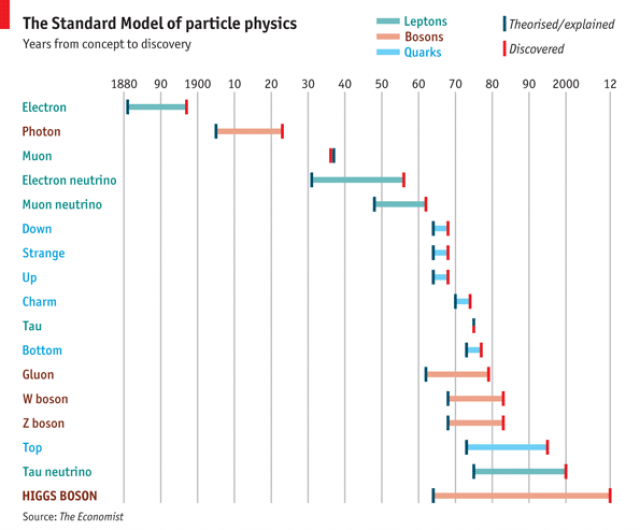
\includegraphics[width=\textwidth]{physics/images/particle_timeline}
\caption{Timeline of particle theorization and discovery}
\end{figure}
Mass difference between initial particle and decay products is the primary factor determining lifetime (smaller the difference, longer the lifetime). When looking at a decay, one can get an idea of the amplitude by multiplying the coulpling constant $g$ for each vertex with that coupling, and $1/(q^2 - m^2)$ for each internal line, where $m$ is the internal line particle.

Nobody chooses to name new particles $\iota$ (iota) since it has a connotation of insignificance.




\section{Leptons}
\subsection{Electron}

\subsection{Muon}

Muons have a lifetime of $10^{-6}$ s, and decay to electrons (with a pair of neutrinos to conserve Lepton number). The have a mass of 105 MeV, about a tenth that of the proton.

Muon does not decay to an electron via photon

Prompt muon decays from $W,Z$ decay.

\subsection{Tau}
Mass of 1.776 GeV and a lifetime of $10^{-13}$. Decay hadronically (mostly to pions) $65\%$ of the time.

\subsection{Neutrino}\label{neutrino}
Looking at products of neutron decay 
\begin{align}
n\rightarrow p^+ + e^-+ \nu_{\bar{e}}
\end{align}
the momentum of the proton and electron is not always back to back. Pauli posited the existence of another particle to save four-momentum conservation. We know it is there because...

Neutrinos are detected after they interact weakly with some material, through exchange of a $W$ or $Z$. The flavor of the neutrino is deduced because after $W$ exchange, you have the corresponding lepton. With that lepton, you can tell what it is from Cherenkov radiation if it is relativistic.

Majorana fermions are their own antiparticle, which neutrinos might be.

\section{Quarks}
Quarks compose Hadrons which is a super group of Mesons (quark-antiquark pair) and Baryons (three quarks).
\begin{itemize}
    \item $u$ - The up quark is the lightest of all the quarks with a mass of only 2.3 MeV, about 4 electrons.
    \item $d$ - The down quark is the second lightest quark with a mass of 4.8 MeV.
    \item $c$ - The charm quark has a mass of 1.29 GeV is the third largest quark, just larger than a proton.
    \item $s$ - The strange quark is the third lightest quark with a mass of only 95 MeV, roughly a muon. Was theorized by Murray Gell-Mann, and found at SLAC in 1968.
    \item $t$ - The top quark is the heaviest quark at 175 GeV, about the size of a tungsten atom. Since it is so heavy it decays with a lifetime of just $10^{-25}s$, which is short than the lifetime of the strong interaction, preventing it from forming hadrons. The only way a single quark can decay is through a $W$ boson, which makes $t\rightarrow Wb$ happen $99.8\%$ of the time. It was postulated in 1973 and found in 1995 at CDF at Fermilab.
    \item $b$ - The bottom quark has a mass of 4.18 GeV, the second largest quark. CKM matrix elements $V_{ub}$ and $V_{cb}$ are suppressed making the lifetime long $10^{-12}$ s. Mesons made of $b$ quarks have algorithms for identification within CMS due from their long lifetime (Section \ref{id-aglos}).
\end{itemize}

\section{Mesons}
Mesons contain both a quark and antiquark pair.

\subsection{Pion}
There are two types of pions charged and uncharged. Each have a mass of roughly 140 MeV, making them a bit larger than a muon. Both have Spin-0
\begin{itemize}
    \item $\pi^+ = u\bar{d}$, $\pi^- = d\bar{u}$. Charged pions mostly ($99.99\%$ of the time) decay weakly to $\mu, \nu_\mu$ with a lifetime of $10^{-8}$ s.
    \item $\pi^0 = u\bar{u}, d\bar{d}$. Mostly ($98.82\%$ of the time) decay electromagnetically to a pair of photons with a shorter lifetime of $10^{-13}$ s
\end{itemize}
Hideki Yukawa in 1935 originally predicted the existence of mesons as the carrier particles of the strong force, which the muon was mistaken to be a year later.

\subsection{$J/\Psi$}

The $J/\Psi = c\bar{c}$ has a mass of 3.1 GeV, about the mass of tritium. The name comes from the near simultaneous discovery in 1974 from both Burton Richter at SLAC ($\Psi$) and Samuel Ting at Brookhaven National Lab ($J$). The lifetime is $10^{-20}$ s, which is very long, since it mostly decays strongly ($10^{-23}$ s). The long lifetime is due to toe OZI Rule (Section \ref{ozi}). $6\%$ branching ratio to muons

\subsection{Kaon}
The Kaon is $K^+ = u\bar{s}, K^0 =( d\bar{s}, \bar{s}d), K^- = \bar{u}s$ and has a mass of 493 MeV, about 5 muons. $64\%$ of charged Kaon's decay to muons.

\section{Baryons}
Baryons contain three quarks

\subsection{Proton}
Proton is the lightest Baryon which prevents it from decay from conservation of Baryon number.

\subsection{Neutron}

A neutron is composed of two down quarks and one up quark making it a "$dud$". 
Lifetime of 15 minutes. Produced in collisions(?), only slowed down through bumping into things of roughly equal size. If it hits a proton, the proton showers and is how the neutron eventually loses energy. The neutron will slow down until it reaches thermal energy of about $1/40 eV$. It then gets absorbed by a nucleus(?) which gives of ~MeV photons, which can then pair produce and make electrons where they shouldn't be. 


\section{Bosons}
\subsection{$W$ Boson}

Mass of 80 GeV. Decays can be found with counting arguments, allowed decays are $e\nu_e, \mu\nu_\mu,\tau\nu_\tau, ud, sc$. The combination $tb$ is not allowed since the $t$ is so heavy. The color combinations make each quark combination have 3 possibilities. Thus if we want to know the branching ratio to $e\nu_e$

\begin{align}
B(W\rightarrow e\nu) = \frac{1}{1+1+1+3+3} = \frac{1}{9}\approx 11\%
\end{align}

\subsection{$Z$ Boson}

Mass of 91 GeV. Can't use the same counting arguments we used for the $W$ because there is different coupling for different fermions. The width of the $Z$ boson is dependent on the number of possile final states into which it can decay, so the measurement of the width is a good probe into the existence of a fourth generation of leptons\cite{bstone}. The relationship between the width and decay modes is as follows:
\begin{itemize}
    \item The uncertainty principle gives us a rule of thumb to relate energy width and time
    \begin{align}
    \Delta E\Delta t\ge \hbar/2
    \end{align}
    According to Bob Cousins, this is the wrong way to think about it, but it is no doubt much easier to remember.
    \item The mean lifetime $\tau$ of the $Z$ is related to it's decay constant $\Gamma$ through
    \begin{align}
    \tau = \frac{1}{\Gamma}
    \end{align}
    \item Putting these two together, we see
    \begin{align}
    \Gamma \propto \Delta E
    \end{align}
    \item Since the decay constant is additive
    \begin{align}
    \Gamma = \Gamma_{ee} + \Gamma_{\mu\mu} + \Gamma_{\nu\nu} +  \ldots
    \end{align}
    We see that if we add another decay channel to the $Z$, we increase the width of the mass itself.
\end{itemize}
The height is proportional to $\frac{\Gamma(Z\rightarrow hadrons)}{\Gamma(Z\rightarrow all)}$ so if there are more leptons, the height will also be reduced. These type of measurements were what LEP (Section \ref{lep}) was used for.

\subsection{Higgs}


\begin{figure}
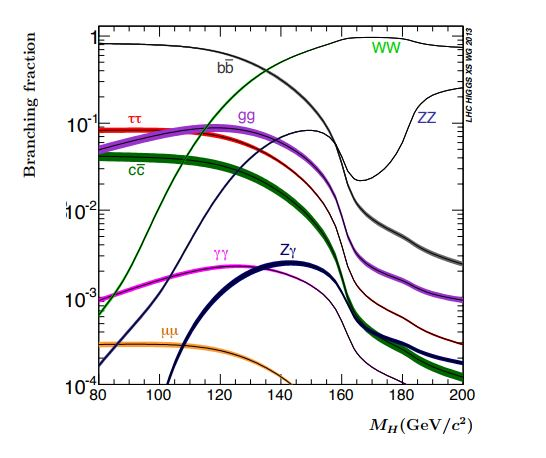
\includegraphics[width=\textwidth]{physics/images/higgs_br.jpg}
\caption{Branching fraction of Highs boson as a function of mass. Fraction to $WW$ is higher than to $ZZ$ at higher $m_H$ due to $Z$'s being identical particles. The branching ratio is exactly a factor of 2 at high mass.}
\end{figure}


With a mass of 125 GeV, the Higgs was the most recent elementary particle to be discovered and was the lynchpin of the Standard Model. Higgs not discovered in earlier colliders because:
\begin{itemize}
    \item Too low center of mass energy
    \item $ee$ collider has small cross-section to Higgs, since coupling is proportional to mass of particle.  $u$ and $d$ are also very light, so also not a great candidates. Need high energy $g$ to make a pair of $t\bar{t}$ to make a $h$
\end{itemize}
Higgs production in proton-proton collisions proceeds in one of four ways:
\begin{enumerate}[label=(\alph*)]
    \item Gluon Fusion, in which two gluons interact via a loop of QCD fermions (top is largest contribution) to produce a single Higgs boson
    
    \item Vector Boson Fusion, in which two quarks radiate a weak boson which fuse and couple directly to a Higgs. This Higgs is produced in association with two jets.
    
    \item Higgs-strahlung, in which a gauge boson produced in the pp collision radiates a Higgs. This Higgs is thus produced in association with the gauge boson.
    
    \item Associated top quark pair production.
\end{enumerate} 

At current LHC energies, $\sqrt{s} = 13 \text{ TeV}$, gluons carry most of the proton's momentum and so Gluon Fusion is the dominant production mechanism, followed by VBF. Below are Feynman diagrams to LO for these production mechanisms:

\begin{center}
    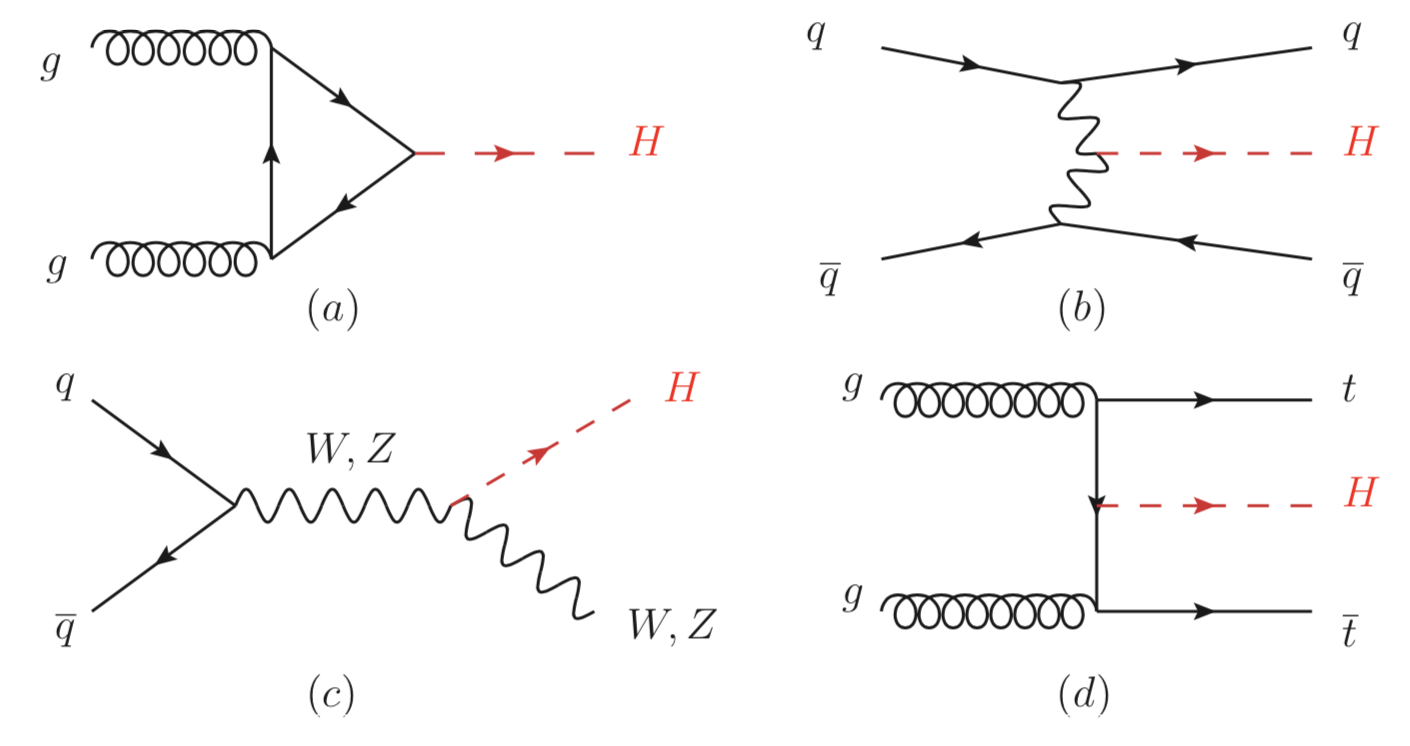
\includegraphics[scale=0.5]{physics/images/higgs_production_diagrams}
\end{center}

While GF dominates Higgs production at LHC energies, other production mechanisms are still important for Higgs analysis. Consider VBF, where the scattered quarks manifest into two hard jets appearing in the forward and backward regions of the detector. Because of the color-singlet nature of the weak-boson exchange, gluon radiation from the central rapidity regions is strongly suppressed. This feature can be exploited to reduce overwhelming QCD backgrounds, including GF-induced Higgs + 2-jet production or $VH$ production with hadronically decaying weak-boson. Thus VBF is valuable as a clean environment for Higgs searches and measurements of Higgs couplings. A typical VBF event includes a Higgs candidate accompanied by two energetic jets ($\geq 30 \text{ GeV}$), with a large dijet mass ($m_{jj} \geq 400\text{ GeV}$) and pseuodrapidity ($\Delta\eta_{jj} \geq 3.5$). However, such a sample does have contamination from GF-produced Higgs.

$VH$ production follows VBF in importance at the LHC, seen primarily as Higgs-strahlung but also in a diagram without a virtual weak boson, in which $ZH$ couples to gluons via a top-quark loop. $VH$ production, together with $t\overline{t}H$ production, provides a relatively clean environment to study Higgs decays into $b$ quarks.

\vspace{1em}
\vspace{1em}
There are five main sets of Higgs final states for which there are searches at the LHC: $b\overline{b}$, $W^+W^-$, $ZZ$, $\gamma \gamma$, and $\tau^+\tau^-$. The following table summarizes the theoretical cross sections for modes of Higgs production and decays:

\begin{center}
    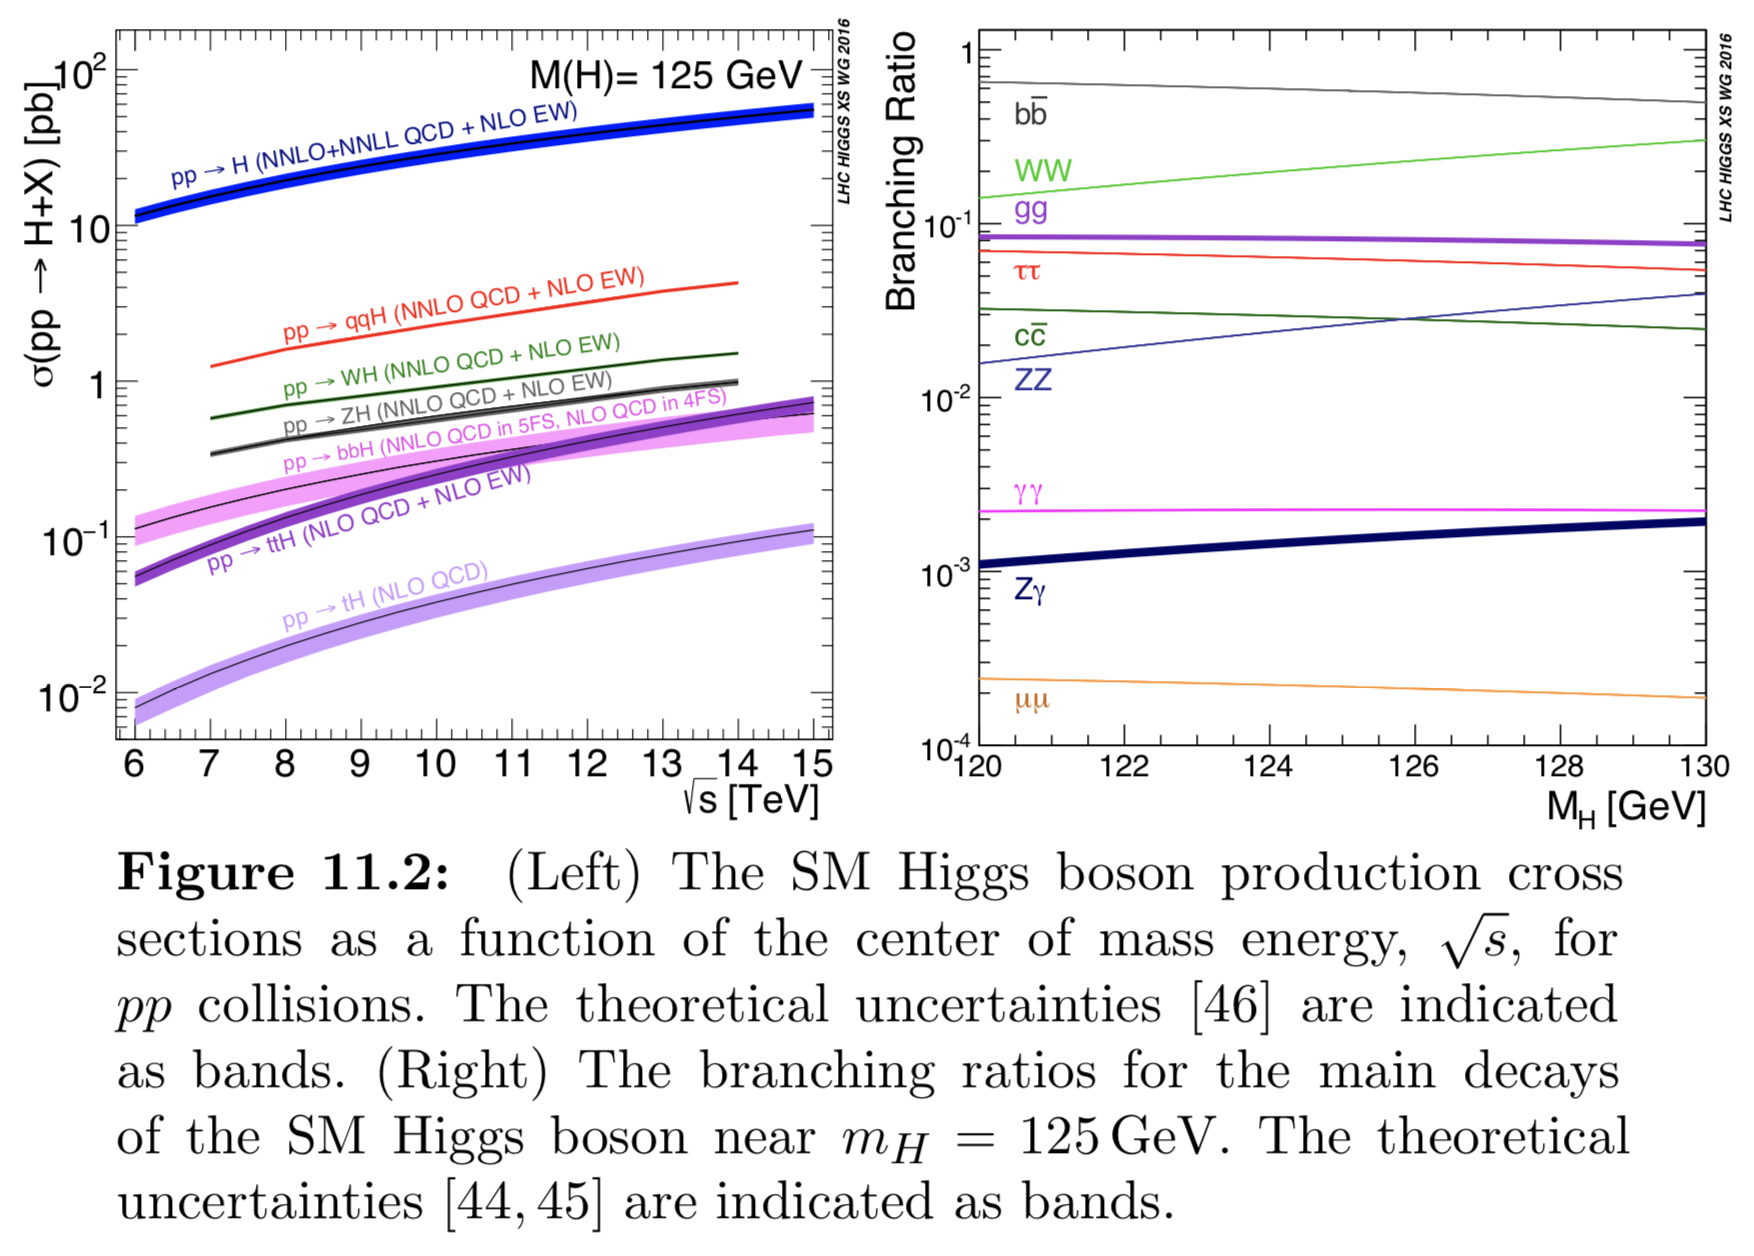
\includegraphics[scale=0.4]{physics/images/higgs_cross_sections}
\end{center}
Consulting the plot on the right, note that the five sets of Higgs final states mentioned before are not the 5 sets with the highest branching ratios for Higgs decays. This is because backgrounds must be considered; the aforementioned five final states are those best optimized to isolate the signals from LHC backgrounds.

On theoretical grounds, for a given $m_H$, the sensitivity of a search channel depends on the production cross section, the branching ratio, the mass resolution, and the backgrounds. For a low-mass Higgs ($110<m_H\text{ (GeV)}<150$), the mass resolutions for the five most important channels are presented in the following table from the PDG:

\begin{center}
    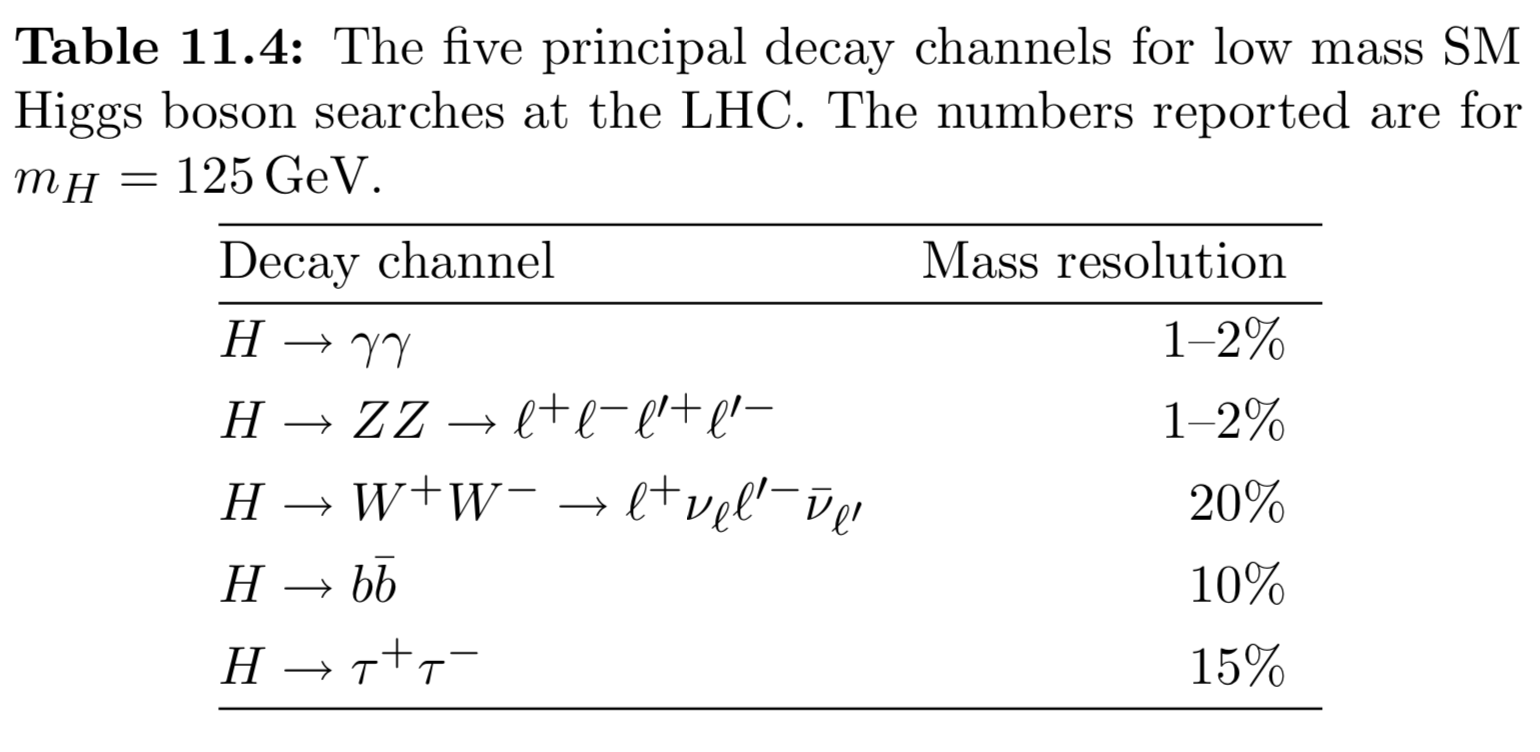
\includegraphics[scale=0.4]{physics/images/higgs_mass_resolution}
\end{center}
When all factors that contribute to a search's sensitivity are considered, $H\rightarrow \gamma \gamma$ and $H\rightarrow ZZ^*\rightarrow 4\ell$ are the best channels for discovery, with excellent mass resolution, well-reducible backgrounds, and precise measurement of all final state particles. Following these at low-mass is $H \rightarrow WW^* \rightarrow \ell \nu \ell \nu$, with a large BR but poor mass resolution due to the presence of two neutrinos as MET. After this are $H\rightarrow b\overline{b}$ and $H\rightarrow \tau \tau$, which have large backgrounds and poor mass resolution.

\vspace{1em}
\vspace{1em}
\noindent \underline{$H \rightarrow \gamma \gamma$}

\vspace{1em}
\noindent A search was performed for a narrow peak over a smoothly falling background in the high $p_T$ diphoton invariant mass distribution $m_{\gamma \gamma}$. The backgrounds are comprised of prompt diphoton, gamma+jets, and dijet processes and are not overwhelming in light of a signal search. To further enhance search sensitivity, events are categorized based on production mechanism: events with high $p_T$ leptons and/or MET consistent with a $W$ or $Z$ decay are tagged in the $VH$ category. Events with diets and a large mass and $\eta$ difference belong to VBF, while remaining events are considered as $VH$ if the jets are compatible with a hadronic $W$ or $Z$, or as GF. The leptonic $VH$ category is quite pure, while VBF has contamination from GF.

\vspace{1em}
\noindent \underline{$H \rightarrow ZZ^* \rightarrow 4l$}

\vspace{1em}
\noindent A search was performed for a narrow peak over a small continuous background dominated by non-resonant $ZZ^*$ production from $qq$ annihilation or $gg$ fusion. Subdominant and reducible backgrounds are $Z+b \overline{b}$, $Z$+jets, and $t \overline{t}$. Lepton isolation and IP cuts are used to suppress these bkg channels. Since the mass resolution and bkg levels are different for the 4$\mu$, 4$e$ and 2$e$ 2$\mu$ subchannels, events are analyzed separately based on the final state leptons and then combined. Furthermore, events are categorized by production mechanism using the same identifiers in the diphoton search.

\vspace{1em}
\noindent Given that we have a 2$e$2$\mu$ event, we prefer to have $Z \rightarrow ee$ and $Z^* \rightarrow \mu \mu$. It is known that the resolutions for detecting both particles follow:


\begin{equation}
\frac{\delta p_T}{p_t} \sim p_T \quad \text{(muons)} \qquad \qquad \
\frac{\delta E}{E} \sim \frac{1}{\sqrt{E}} \quad \text{(electrons)}
\end{equation}
From this, we conclude that we desire lower energy muons so that we may better measure their curvature (and thus $p_T$) and higher energy electrons for better resolution.

\vspace{1em}
\noindent \underline{$H \rightarrow W^+W^- \rightarrow l \nu l \nu$}

\vspace{1em}
\noindent While the production rate is large, the mass resolution is poor due to two neutrinos, and the backgrounds are numerous. Events are divided based on the lepton flavor combination and the number of jets. Background reduction and estimation is vital in this search. For events with opposite-flavor lepton and no accompanying high $p_T$ jets, the dominant background stems from non-resonant $WW$ production. Events with same flavor leptons have large Drell-Yan contamination. $Wt$, $W$+jets (with jet misidentified as a lepton), and $t\overline{t}$ contaminate all categories \cite{bstone}.

\chapter{Experimental Particle Physics}
Difference between radiation length $\chi_0$ and stopping power $dE/dx$

\section{Passage of Particles through Matter}

A muon is minimum ionizing from $0.1\le \beta\gamma \le 1000$ or equivalently $10$ MeV $\le p\le 100$ GeV. A minimum ionizing muon typically loses 2 MeV $cm^2/g$ through a material. Some typical materials

\begin{center}
    \begin{tabular}{ | c | c| c |} 
        \hline
        Material & Density (g/cm$^3$) & MIP Energy Loss \\ \hline
        Iron & 8 & 16 GeV/m \\
        Air & 0.00125 & 0.25 MeV / m \\
        \hline
    \end{tabular}
\end{center}


\subsection{Radiation Length}
Characterizes a material. Distance over which 
\begin{itemize}
    \item Electron is reduced to $1/e$ of it's initial energy
    \item 7/9 the mean free path of a photon before it pair produces
\end{itemize}
Typically measured in $g/cm^2$, so need to divide by the density to get the correct value. This is done since the density of a material is variable.

\begin{center}
    \begin{tabular}{ | c | c|} 
        \hline
        Material & $X_0$ (cm) \\ \hline
        Iron & 1.75 \\
        Lead Tungstate & 0.89 \\
        Water & 36.08 \\
        Air & 30.39 \\
        \hline
    \end{tabular}
\end{center}



\subsection{Multiple Scattering}
For relativistic particles, the angle $\theta$ scattered in a material is
\begin{align}
\theta \approx \frac{13.6 \textrm{MeV}}{\beta c p}z\sqrt{\frac{X}{X_0}}
\end{align}
Where $p,z$ is the momentum and charge respectively of the incident particle. $X$ is the distance travelled in the medium with radiation length $X_0$. Becomes less and less relevant as particle momentum increases (depends on $1/p$)

\subsection{Bremsstrahlung}
 An electron loses most of its energy through Bremsstrahlung at energies $\ge 10$ MeV. Electron energy loss by Brem $\propto E_e$, loss by ionization $\propto \ln E_e$. Shower length is roughly twice that of the radiation length of a material \cite{pdg} The critical energy of a muon in Iron (i.e. the energy at which Radiative losses are equal to Ionization losses) is $E_{\mu c} = 332$ GeV. Muon energy loss goes as 
 \begin{align}
 -dE/dx = a(E) + b(E)E
 \end{align}
 $a(E)\approx 0.002$ g$^{-1}$cm$^2$ is from ionization energy loss, $b(E)$ is from brem, pair production, etc.
\subsection{Cascade Showers}

Electromagnetic showers caused by Bremstrallung which creates high energy photon, which then pair produces, and the products of which then brem high energy photons, etc until everything is out of energy.

Transverse development of a shower is parametrized by the Moliere radius $R_M$


\begin{align}
R_M = X_0E_s/E_c
\end{align}

Electrons only? $E_s = 21$ MeV is the "scale" energy? Only 10$\%$ of the energy lies outside of the cylinder of this size, $99\%$ is within 3.5$R_M$. 

\subsection{Pair Production}
Electron pairs are produced by photons in the electric field created by the nucleus. Pairs take energy, nucleus balances momentum. (Rossi pg. 13)

\subsection{Landau-Pomeranchuk-Migdal (LPM) Effect}
For very high energy particles, neighboring nuclei get squished which causes a suppression of both bremsstrahlung and pair-production.



\section{Symmetries}
\subsection{Parity}
Parity inversion is the flip of the sign of all three spatial coordinates of a system. Effectively what it does is change something into it's mirror image. The symmetry assumes that if the world were actually it's mirror image (i.e. everything that was once "left" becomes "right"), all of the Physics would remain exactly the same. This symmetry can be tested for by looking at the \textbf{helicity} associated with an interaction
\begin{align}
h = \textbf{S}\cdot\textbf{p}
\end{align}
Under parity inversion, the momentum of a particle changes sign (vector), whereas the spin does not (axial vector). This causes the helicity to change sign under parity inversion. If an interaction respects the symmetry of parity inversion, the average of this quantity should come out to be zero, since if it did not, it would imply that the real world, and the "mirror image" world would be different from each other.

Madame Wu led an experiment that looked at beta decays from cold Cobalt-60 atoms which had their spins aligned in a uniform magnetic field. This gave the direction of the $\textbf{S}$ vector used in the Helicity measurement. From here, all that was left to do was measure the direction which the electron was emitted, effectively upwards or downwards relative to the spin of the nucleus. If parity was not violated, helicity should average to zero, which means one should see the same amount going up as down.

The Cobalt subsequently decayed electromagnetically through two $\gamma$'s. The electromagnetic interaction was known to respect parity conservation, so they used the photons to measure how polarized they were able to get the Cobalt atoms initially. The direction of the photons gave the direction of the nuclear spin. If the electron decay was parity invariant, the electrons should be found on average to have no correlation with the direction of the emitted photons. It was found that they tracked exactly opposite this direction revealing the weak force to \emph{maximally} violate parity.

\begin{align}
\langle h \rangle = \langle \textbf{S}\cdot\textbf{p} \rangle \neq 0
\end{align}

For a massive particle, the helicity is not Lorentz invariant, since it is always possible to boost to a frame in which the momentum vector changes, while the direction of spin does not. The \textbf{chirality} of a particle tells us how a particle transforms in the right- or left-handed representation of the Poincare group. For massless particles this is the same as helicity, but is different for things with mass. Only left-handed fermions and right-handed antifermions interact with the weak-interaction.



\section{Experimental Conservation Laws}

\begin{itemize}
    \item Conservation of Charge - 
    \item Conservation of Leptons - Amount of electrons, muons, taus always conserved, keeping count with neutrinos, etc.
    \item Conservation of Color - At a strong vertex the quark color changes (there are three), the difference is carried by the gluon.
    \item Conservation of Baryon number - amount of quarks are always conserved. Cabbibo mixing lets quarks change generations
    \item $\sim$ Conservation of Flavor - not a real conservation law, but mostly true, conserved in strong and electromagnetic decays, not weak decays
\end{itemize}
Lepton number is conserved because...

Spin affects particle decays, if a spin-0 particle decays, it is isotropic. Weak decays, since they violate parity, decay preferentially in the direction along the axis of their momentum (?)


Most of the time, lepton flavor is conserved except in neutrino oscillations.

\section{Particle Detection}
\subsection{Cherenkov Radiation}
Happens when a particle travels faster than the speed of light does within a particular medium. It is characterized by a "cone" which makes a angle dependent on the speed of the particle producing the light
\begin{align}
\cos\theta =\frac{1}{n\beta}
\end{align}
Where $n$ is the index of refraction of the medium, and $\beta = v/c$ of the particle.


\section{Cross Section and Luminosity}
First we define the instantaneous luminosity (typically just called the \textbf{luminosity}) of a beam of particles as \cite{cousins}
\begin{align}
\mathcal{L} = \textrm{number~of~incident~particles~per~unit~area,~per~unit~time}
\end{align}

We use this as a metric for how much beam we have. We don't just want the number of particles per unit time because it wouldn't tell us how concentrated our beam is.  Typical values of the instantaneous LHC (circa August 2018) are
\begin{align}
\mathcal{L}_{LHC} &\approx 2\times 10^{38} /m^2s
\end{align}
To get an understanding of this number, the diameter of a human hair is roughly  100 $\mu m$, so
\begin{align}
\textrm{cross section of human hair} \approx   10^4 \mu m^2
\end{align}
A mole of atoms is of course $10^{23}$, so putting it all together
\begin{align}
\mathcal{L}_{LHC} \approx 20 \textrm{~moles / hair~} \mu s
\end{align}
We are shooting about 20 moles worth of protons through an area the size of a human hair every microsecond.

When we shoot two beams together, or a beam at a wall, we generally care about how many of these particles (per unit time) get scattered, i.e smash into each other and go flying off. We write this value as $dN/dt$ and is related to the instantaneous luminosity with

\begin{align}
\frac{dN}{dt} = \sigma\mathcal{L}
\end{align}
Where $\sigma$ is called the \textbf{cross section} for the collision to occur, having units of area. The larger the cross section, the more scattered particles you will get. In actuality, one counts how many scattered particles show up at each angle, giving us a differential $\sigma$, which is then integrated over all angles to get the full cross section \cite{griffiths_qm}.


Another common value is the \textbf{integrated luminosity} which is simply the instantaneous luminosity added up over some period of time. With this, we can calculate how many scattered particles we had over a given time
\begin{align}
N = \sigma \int \mathcal{L}~dt
\end{align}

Integrated luminosity effectively tells us how many particles have passed through the collision point.  Units are inverse "barns" (1 barn = 100 fm$^2$), which was supposed to be a large area (size of a typical nucleus) concerning nuclear interactions. Integrated luminosity tells us, if we were to put all the particles that passed through the interaction point all there at once, how dense the plane would be filled with these particles. As you increase integrated luminosity, you decrease the scale (i.e. $pb^{-1} \rightarrow fb^{-1}$) which shows that the density of particles is increasing. Integrated luminosity of the LHC is given as

\begin{center}
\begin{tabular}{ | c | c|} 
\hline
 Year & $\int \mathcal{L} dt$ [$fb^{-1}$] \\ \hline
 2018 & 67.86  \\ 
 2017 & 49.79  \\
2016 & 37.80   \\ 
2015 & 4.21 \\
2012 & 21.79 \\
2011 & 5.55\\
\hline
\end{tabular}
\end{center}

\section{Famous Experiments}

\subsection{LEP}\label{lep}
The Large Electron Positron Collider was used 1989-2000 at CERN. With an energy of 209 GeV, was used for precision data on the $Z$ and $W$ boson. It was a circular collider with a 27 km circumference.
\subsection{CDF}
Proton-antiproton collider at Fermilab (Collider Detector at Fermilab). Got to about $2$ TeV center of mass energy, was where the top quark was discovered.

\subsection{CMS}


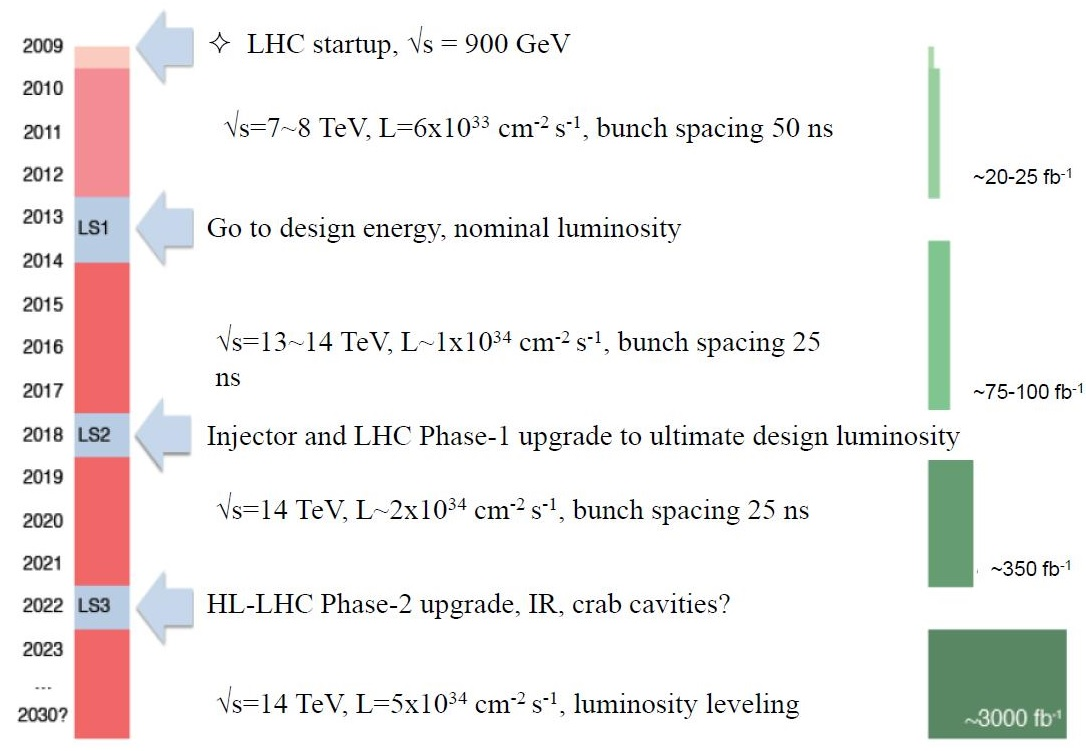
\includegraphics[width=1.0\textwidth]{physics/images/lhc_timeline}


\subsection{Types of Searches}
\begin{itemize}
    \item Long lived neutral particles that decay into muons (detected in muon system, but have displaced vertex)
    \item Long lived charge particles, if they have a large mass, will go slower, can detect through timing (takes longer to get to muon system)
\end{itemize}

\subsection{Pseudorapidity}
The pseudorapidity $\eta$ is used in CMS as a coordinate that directly maps to the angle $\theta$ of a particle relative to the beam line.
\begin{align}
\eta = -\ln\left[\tan\frac{\theta}{2}\right]
\end{align}
It is useful because particle production is large closer to the beam line, and slices of $\eta$ are roughly equally populated whereas slices of $\theta$ are not. Additionally differences in $\eta$ are Lorentz invariant.


\bibliography{references}{}
\bibliographystyle{plain}


\end{document}